\documentclass[10pt]{article}
\usepackage[margin=0.72in]{geometry}
\usepackage{booktabs,longtable,graphicx,subcaption,array,xcolor,hyperref,siunitx,amsmath}
\usepackage[T1]{fontenc}
\hypersetup{colorlinks=true,linkcolor=blue,urlcolor=blue}
\newcommand{\datasetunit}{dataset load unit}
\title{Variable-Level Semantic and Behavioural Audit of the Long-Horizon Forecasting Benchmarks}
\author{}
\date{}
\begin{document}
\maketitle

\begin{abstract}
This audit describes what each benchmark channel measures before treating it as a forecasting coordinate. It combines source documentation with statistics computed directly from the CSV files used by this repository. We report raw ranges, means, standard deviations, dominant periods, cross-variable relations, representative windows, and modelling implications. Missing sentinels are excluded rather than interpreted as physical measurements. The analysis is descriptive: correlation, spectral prominence, and clustering do not by themselves establish physical causation.
\end{abstract}

\section{Audit protocol}
All numerical results are generated by \texttt{dataset\_audit/audit.py}. Means and standard deviations use all finite local observations (population standard deviation). Dominant period is the strongest FFT period after linear detrending and Hann tapering, searched from four samples to 60 days. ``Representative week'' means the non-overlapping seven-day block whose mean, standard deviation, and mean absolute first difference are jointly closest to the componentwise median block. ETT lead/lag uses first differences and searches $\pm48$ hours; a positive lag means that load changes lead oil-temperature changes. For the anonymous panels, $\rho_{24}$ and $\rho_{168}$ are hourly lag correlations. Nearly constant means channel standard deviation below 1\% of the median nonzero channel standard deviation. Highly volatile means normalized first-difference roughness above the Tukey upper fence. These fixed, data-independent definitions prevent post-hoc visual labels.

\paragraph{Semantic sources and local transformations.}
ETT names and collection details follow the official ETT repository (\url{https://github.com/zhouhaoyi/ETDataset}). Weather meanings and units follow the MPI Biogeochemistry weather-station documentation (\url{https://www.bgc-jena.mpg.de/wetter/Weatherstation.pdf}). Electricity semantics follow the UCI ElectricityLoadDiagrams20112014 record (\url{https://archive.ics.uci.edu/dataset/321/electricityloaddiagrams20112014}). Traffic is an hourly processed panel of PeMS detector occupancy; PeMS measures detector occupancy and the UCI PeMS description defines occupancy as a fraction between zero and one (\url{https://archive.ics.uci.edu/dataset/204/pems_sf}). Dates, channel counts, and all values below are taken from the local benchmark files, which may be resampled or relabelled versions of their source archives.

\paragraph{The overloaded \texttt{OT} label.}
\texttt{OT} means oil temperature only in ETT. From the local Weather values and source-column order, we infer that its \texttt{OT} is the source CO2 channel renamed for a common loader; the repository contains no retained conversion manifest that proves the rename directly. Likewise, Electricity \texttt{OT} is the final anonymous client (original index 320) and Traffic \texttt{OT} is the final anonymous detector (original index 861). Neither is an oil-temperature target. This distinction matters for both interpretation and leakage audits.


\section{Electricity Transformer Temperature datasets}

ETTh1/ETTh2 are hourly and ETTm1/ETTm2 are 15-minute records from two transformer stations. Each contains six external load measurements and transformer oil temperature. High, middle, and low distinguish the three load groups; useful and useless are the source archive's names for load components that do and do not contribute to useful transfer. The archive does not expose enough station wiring metadata to equate these labels unambiguously with particular voltage sides or to assert an exact active/reactive-power mapping. It also does not publish an engineering unit for the six load columns; we therefore retain \datasetunit{} rather than inventing kW or kVAr. Oil temperature is reported in degrees Celsius. ETTm1 corresponds to station 1 and ETTm2 to station 2, so the minute/hour pairs should resemble one another while station 1 and station 2 need not share ranges.

\subsection{ETTh1}

The local file contains 17,420 observations from 2016-07-01 00:00:00 to 2018-06-26 19:00:00 at 1-hour cadence. Table~\ref{tab:etth1} reports unnormalized values.

\begin{table}[ht]
\centering\scriptsize
\caption{ETTh1 variable semantics and empirical behaviour.}\label{tab:etth1}
\resizebox{\textwidth}{!}{%
\begin{tabular}{lllrrl}
\toprule
Variable & Meaning & Unit & Min--Max & Mean $\pm$ Std & Dominant period \\
\midrule
HUFL & High useful load & dataset load unit & -22.706--23.644 & 7.375 $\pm$ 7.068 & 24.0 h (daily) \\
HULL & High useless load & dataset load unit & -4.756--10.114 & 2.242 $\pm$ 2.042 & 24.0 h (daily) \\
MUFL & Middle useful load & dataset load unit & -25.088--17.341 & 4.300 $\pm$ 6.827 & 24.0 h (daily) \\
MULL & Middle useless load & dataset load unit & -5.934--7.747 & 0.882 $\pm$ 1.809 & 24.0 h (daily) \\
LUFL & Low useful load & dataset load unit & -1.188--8.498 & 3.066 $\pm$ 1.164 & 12.0 h (sub-daily) \\
LULL & Low useless load & dataset load unit & -1.371--3.046 & 0.857 $\pm$ 0.600 & 1161.3 h (long-cycle (48.4 d)) \\
OT & Transformer oil temperature (forecast target) & degree C & -4.080--46.007 & 13.325 $\pm$ 8.567 & 24.0 h (daily) \\
\bottomrule
\end{tabular}}
\end{table}

\begin{table}[ht]
\centering\small
\caption{ETTh1 load--oil-temperature relations. Level correlation is contemporaneous; lag is selected on first differences.}\label{tab:etth1lags}
\begin{tabular}{lrrlr}
\toprule
Load & Level $\rho$ & Best lag (h) & Direction & Change $\rho$ \\
\midrule
HUFL & 0.060 & 2.0 & load leads & -0.129 \\
HULL & 0.224 & 20.0 & load leads & -0.085 \\
MUFL & 0.051 & 2.0 & load leads & -0.132 \\
MULL & 0.220 & 20.0 & load leads & -0.090 \\
LUFL & 0.119 & 21.0 & load leads & 0.043 \\
LULL & 0.067 & -3.0 & load lags & -0.040 \\
\bottomrule
\end{tabular}
\end{table}

\begin{figure}[ht]
\centering
\begin{subfigure}{.49\textwidth}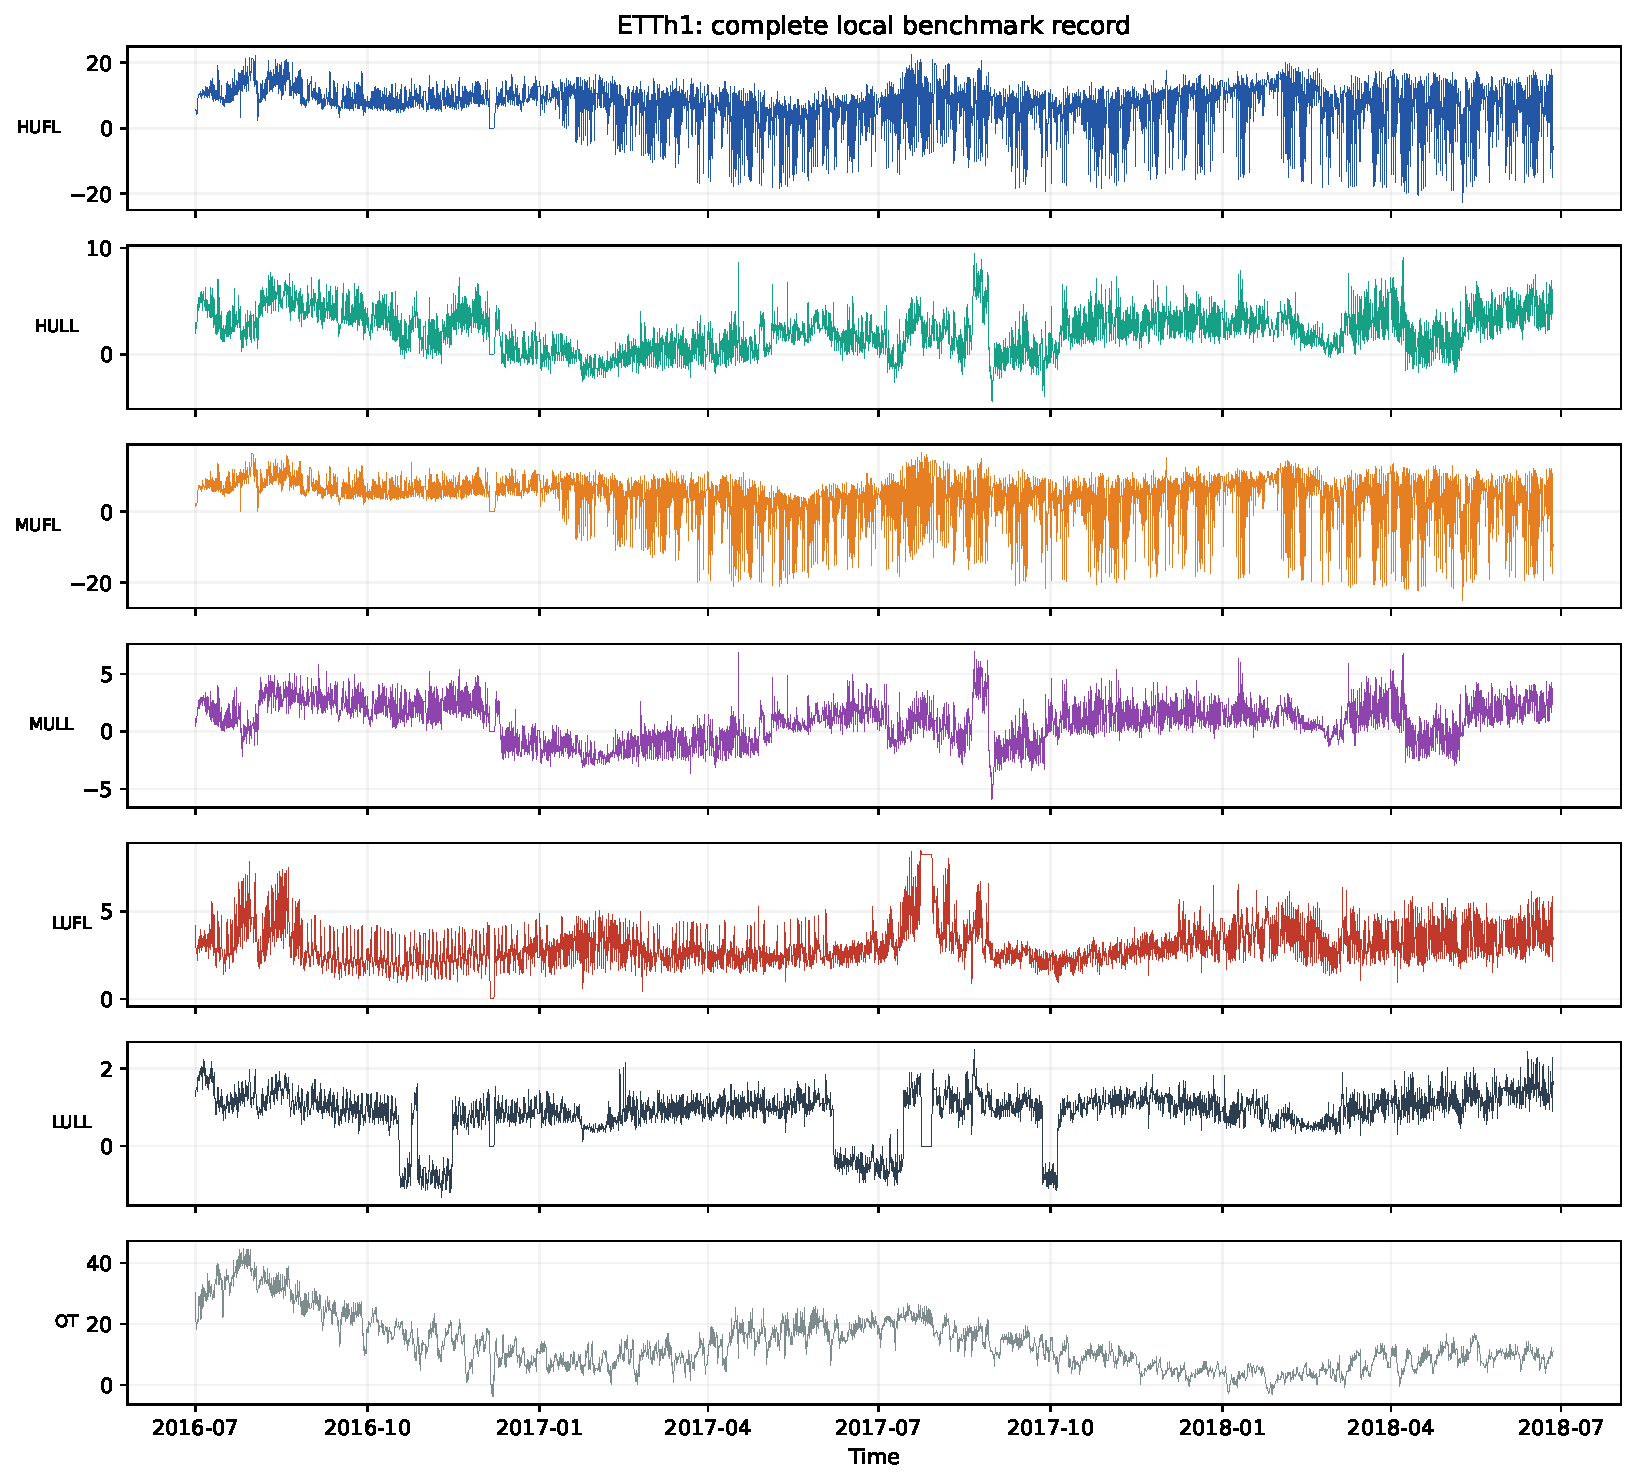
\includegraphics[width=\linewidth]{figures/ETTh1_full.pdf}\caption{Complete record.}\end{subfigure}
\begin{subfigure}{.49\textwidth}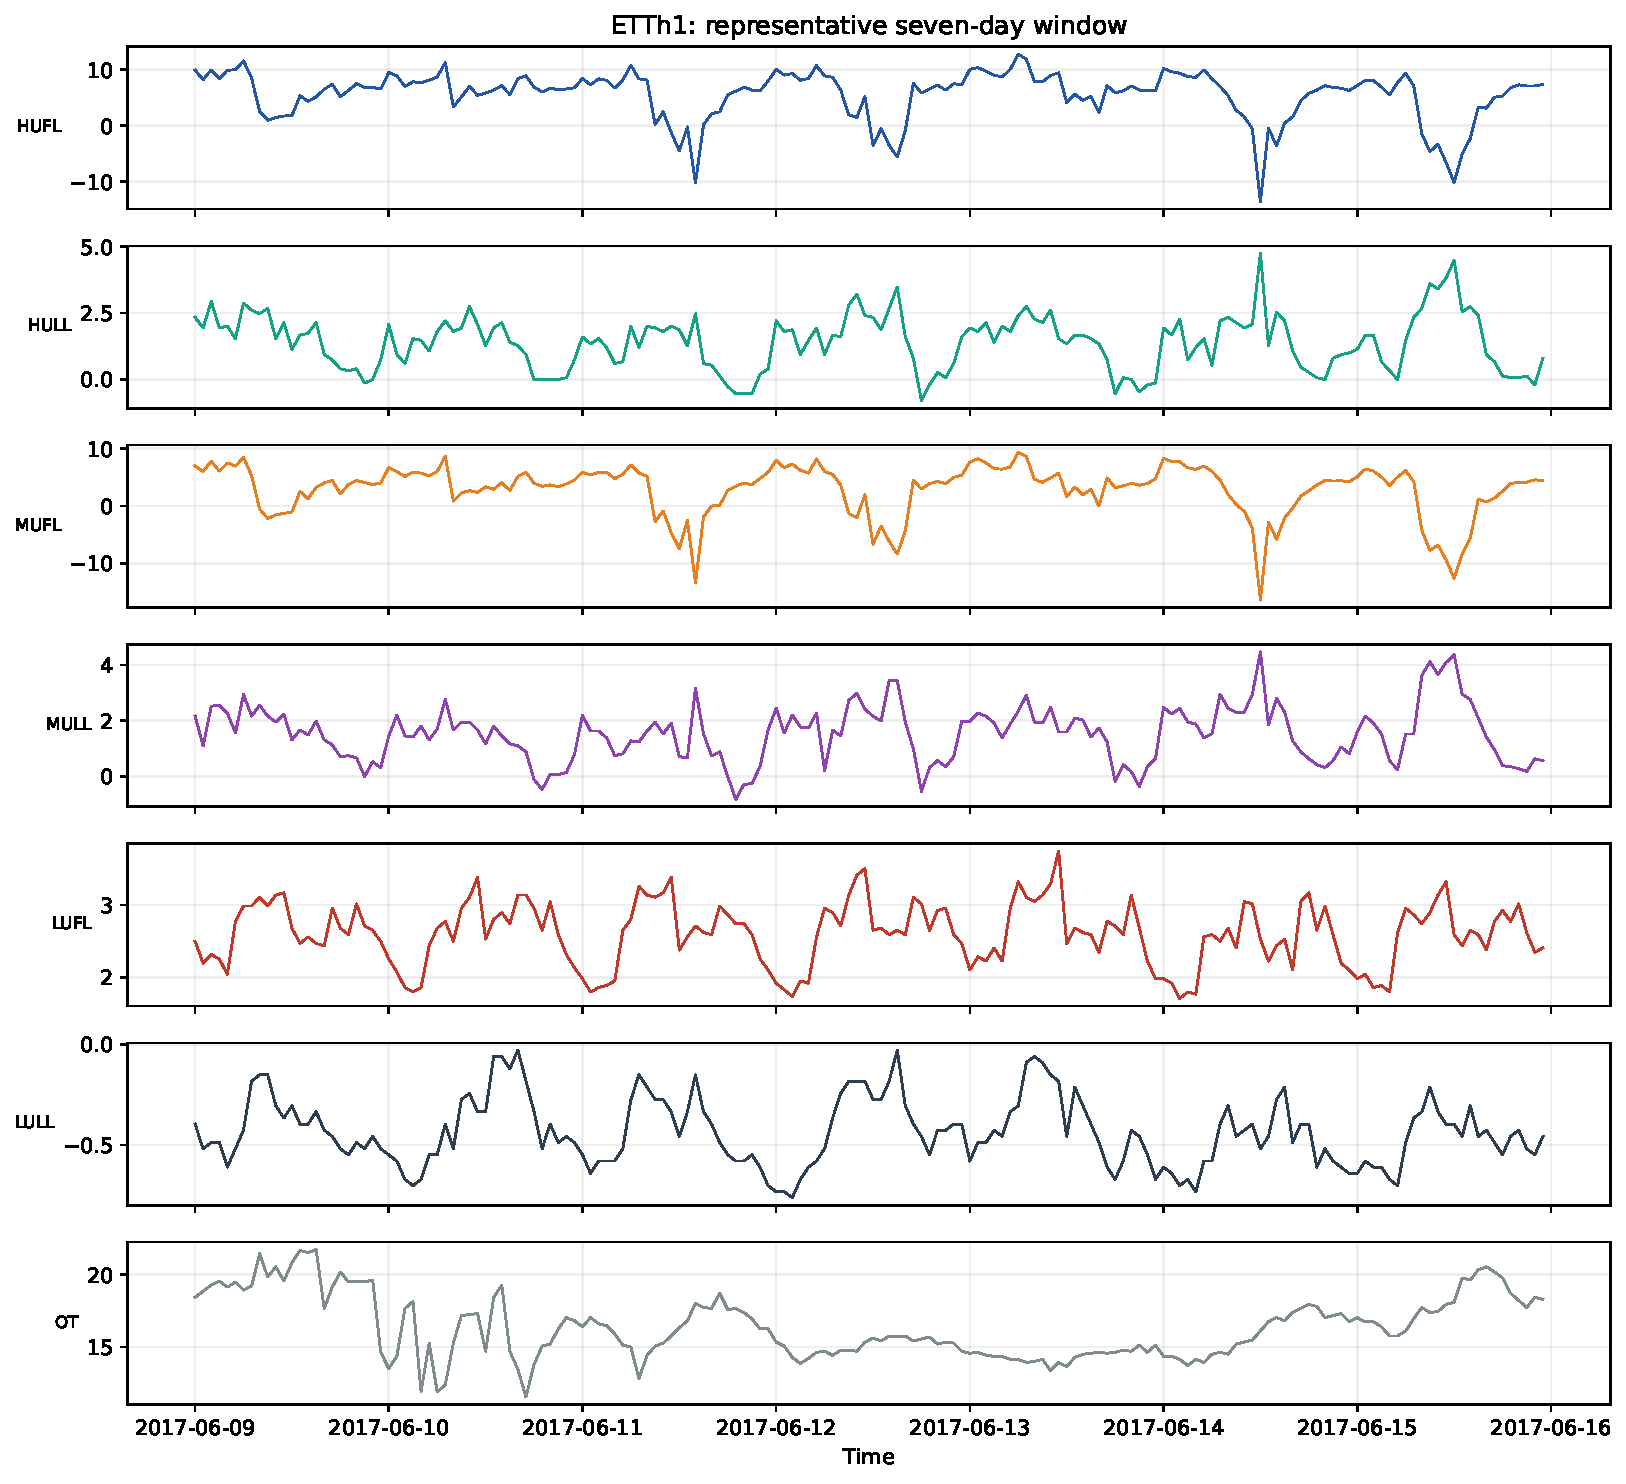
\includegraphics[width=\linewidth]{figures/ETTh1_week.pdf}\caption{Representative seven-day window.}\end{subfigure}
\caption{ETTh1 raw trajectories.}\label{fig:etth1}
\end{figure}

\subsection{ETTh2}

The local file contains 17,420 observations from 2016-07-01 00:00:00 to 2018-06-26 19:00:00 at 1-hour cadence. Table~\ref{tab:etth2} reports unnormalized values.

\begin{table}[ht]
\centering\scriptsize
\caption{ETTh2 variable semantics and empirical behaviour.}\label{tab:etth2}
\resizebox{\textwidth}{!}{%
\begin{tabular}{lllrrl}
\toprule
Variable & Meaning & Unit & Min--Max & Mean $\pm$ Std & Dominant period \\
\midrule
HUFL & High useful load & dataset load unit & 0.000--107.893 & 37.193 $\pm$ 10.219 & 24.0 h (daily) \\
HULL & High useless load & dataset load unit & -18.680--36.439 & 8.538 $\pm$ 6.020 & 967.8 h (long-cycle (40.3 d)) \\
MUFL & Middle useful load & dataset load unit & 11.205--93.230 & 43.830 $\pm$ 13.056 & 1340.0 h (long-cycle (55.8 d)) \\
MULL & Middle useless load & dataset load unit & -6.594--28.736 & 8.323 $\pm$ 4.366 & 483.9 h (long-cycle (20.2 d)) \\
LUFL & Low useful load & dataset load unit & -14.350--17.218 & -3.424 $\pm$ 6.144 & 791.8 h (long-cycle (33.0 d)) \\
LULL & Low useless load & dataset load unit & -31.462--2.932 & -2.086 $\pm$ 6.013 & 1340.0 h (long-cycle (55.8 d)) \\
OT & Transformer oil temperature (forecast target) & degree C & -2.647--58.877 & 26.609 $\pm$ 11.888 & 24.0 h (daily) \\
\bottomrule
\end{tabular}}
\end{table}

\begin{table}[ht]
\centering\small
\caption{ETTh2 load--oil-temperature relations. Level correlation is contemporaneous; lag is selected on first differences.}\label{tab:etth2lags}
\begin{tabular}{lrrlr}
\toprule
Load & Level $\rho$ & Best lag (h) & Direction & Change $\rho$ \\
\midrule
HUFL & 0.035 & 35.0 & load leads & -0.161 \\
HULL & 0.338 & 0.0 & synchronous & 0.071 \\
MUFL & 0.194 & 35.0 & load leads & -0.165 \\
MULL & 0.495 & 0.0 & synchronous & 0.084 \\
LUFL & -0.144 & 2.0 & load leads & -0.100 \\
LULL & -0.112 & -30.0 & load lags & 0.060 \\
\bottomrule
\end{tabular}
\end{table}

\begin{figure}[ht]
\centering
\begin{subfigure}{.49\textwidth}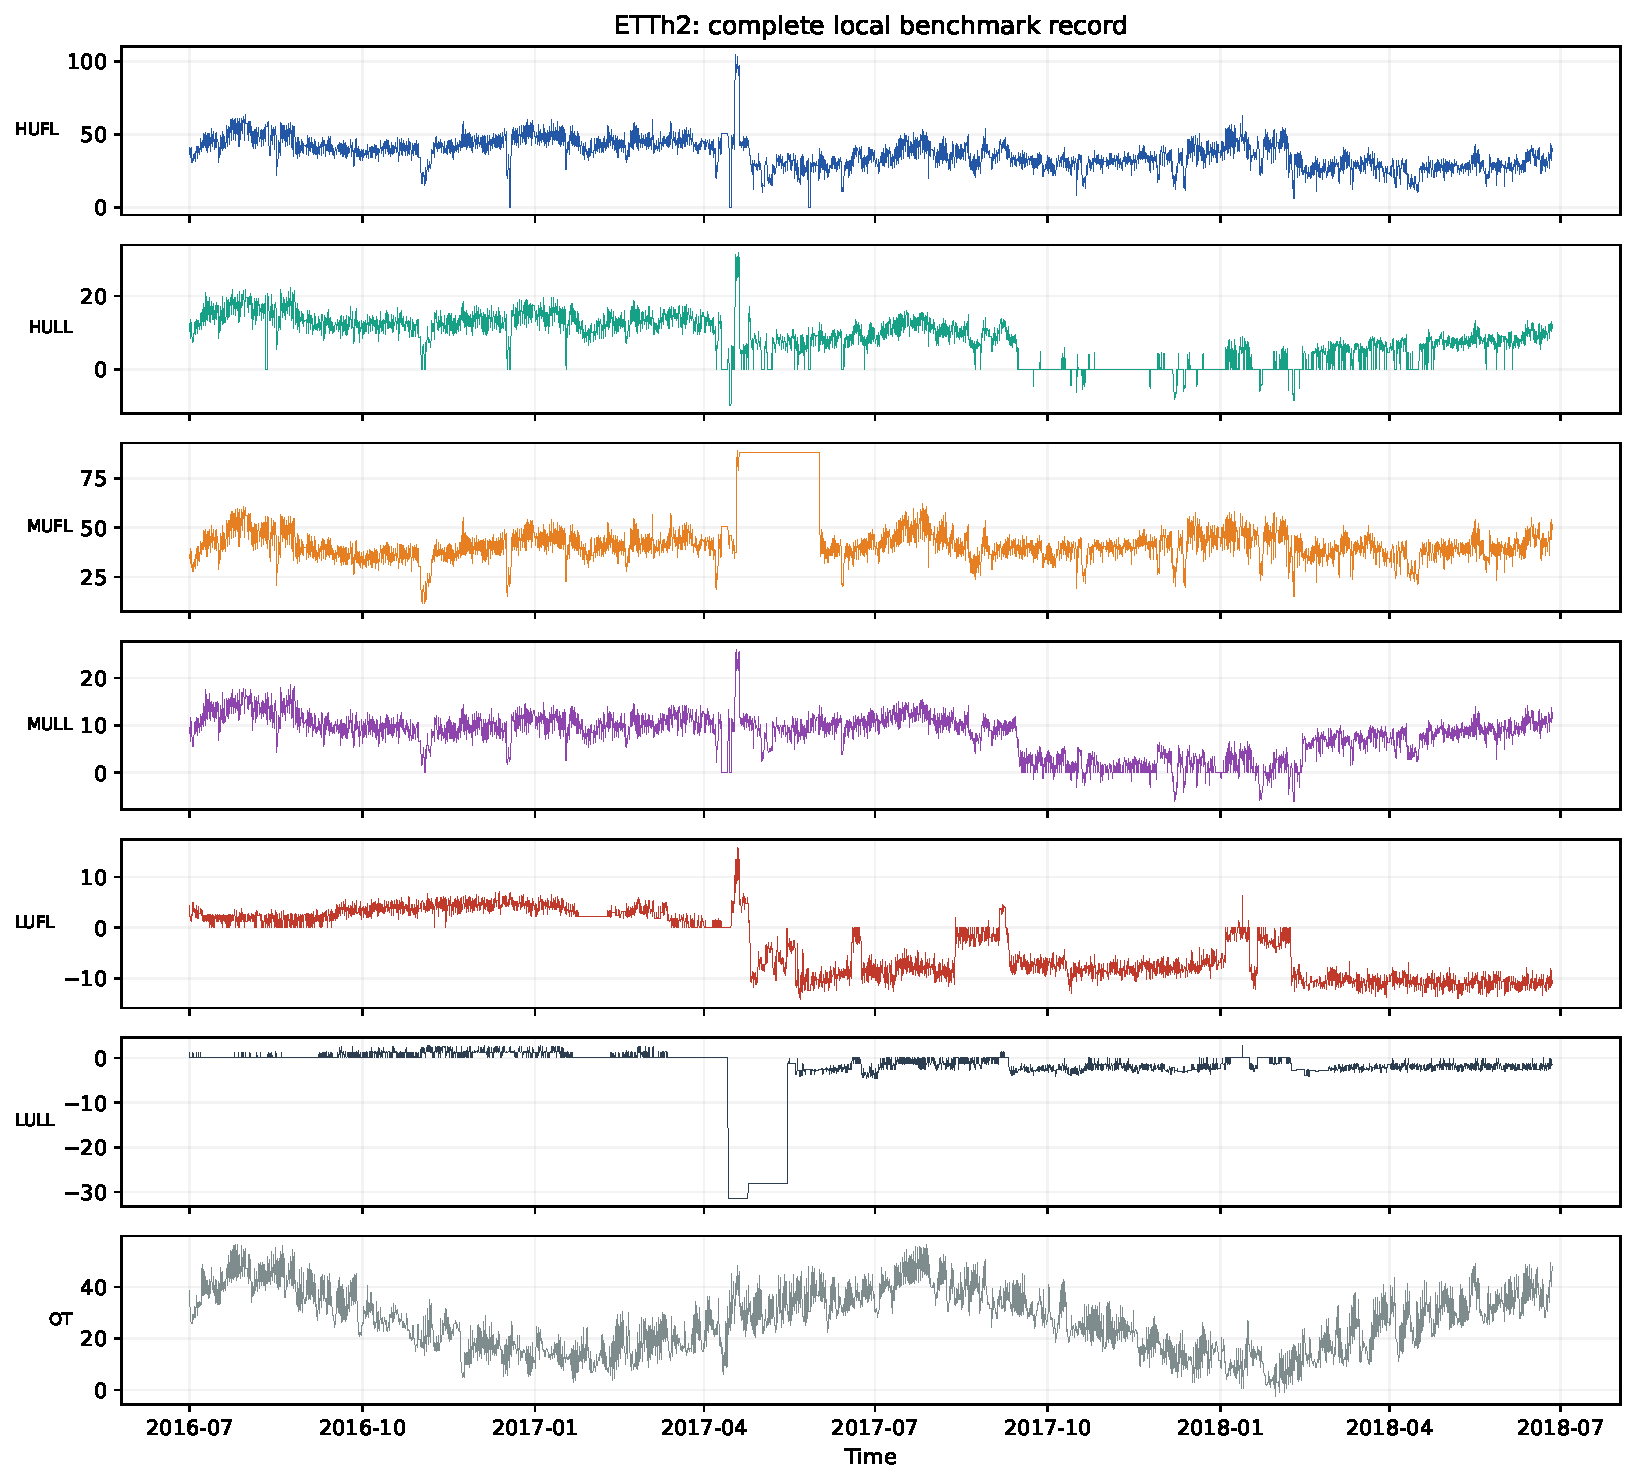
\includegraphics[width=\linewidth]{figures/ETTh2_full.pdf}\caption{Complete record.}\end{subfigure}
\begin{subfigure}{.49\textwidth}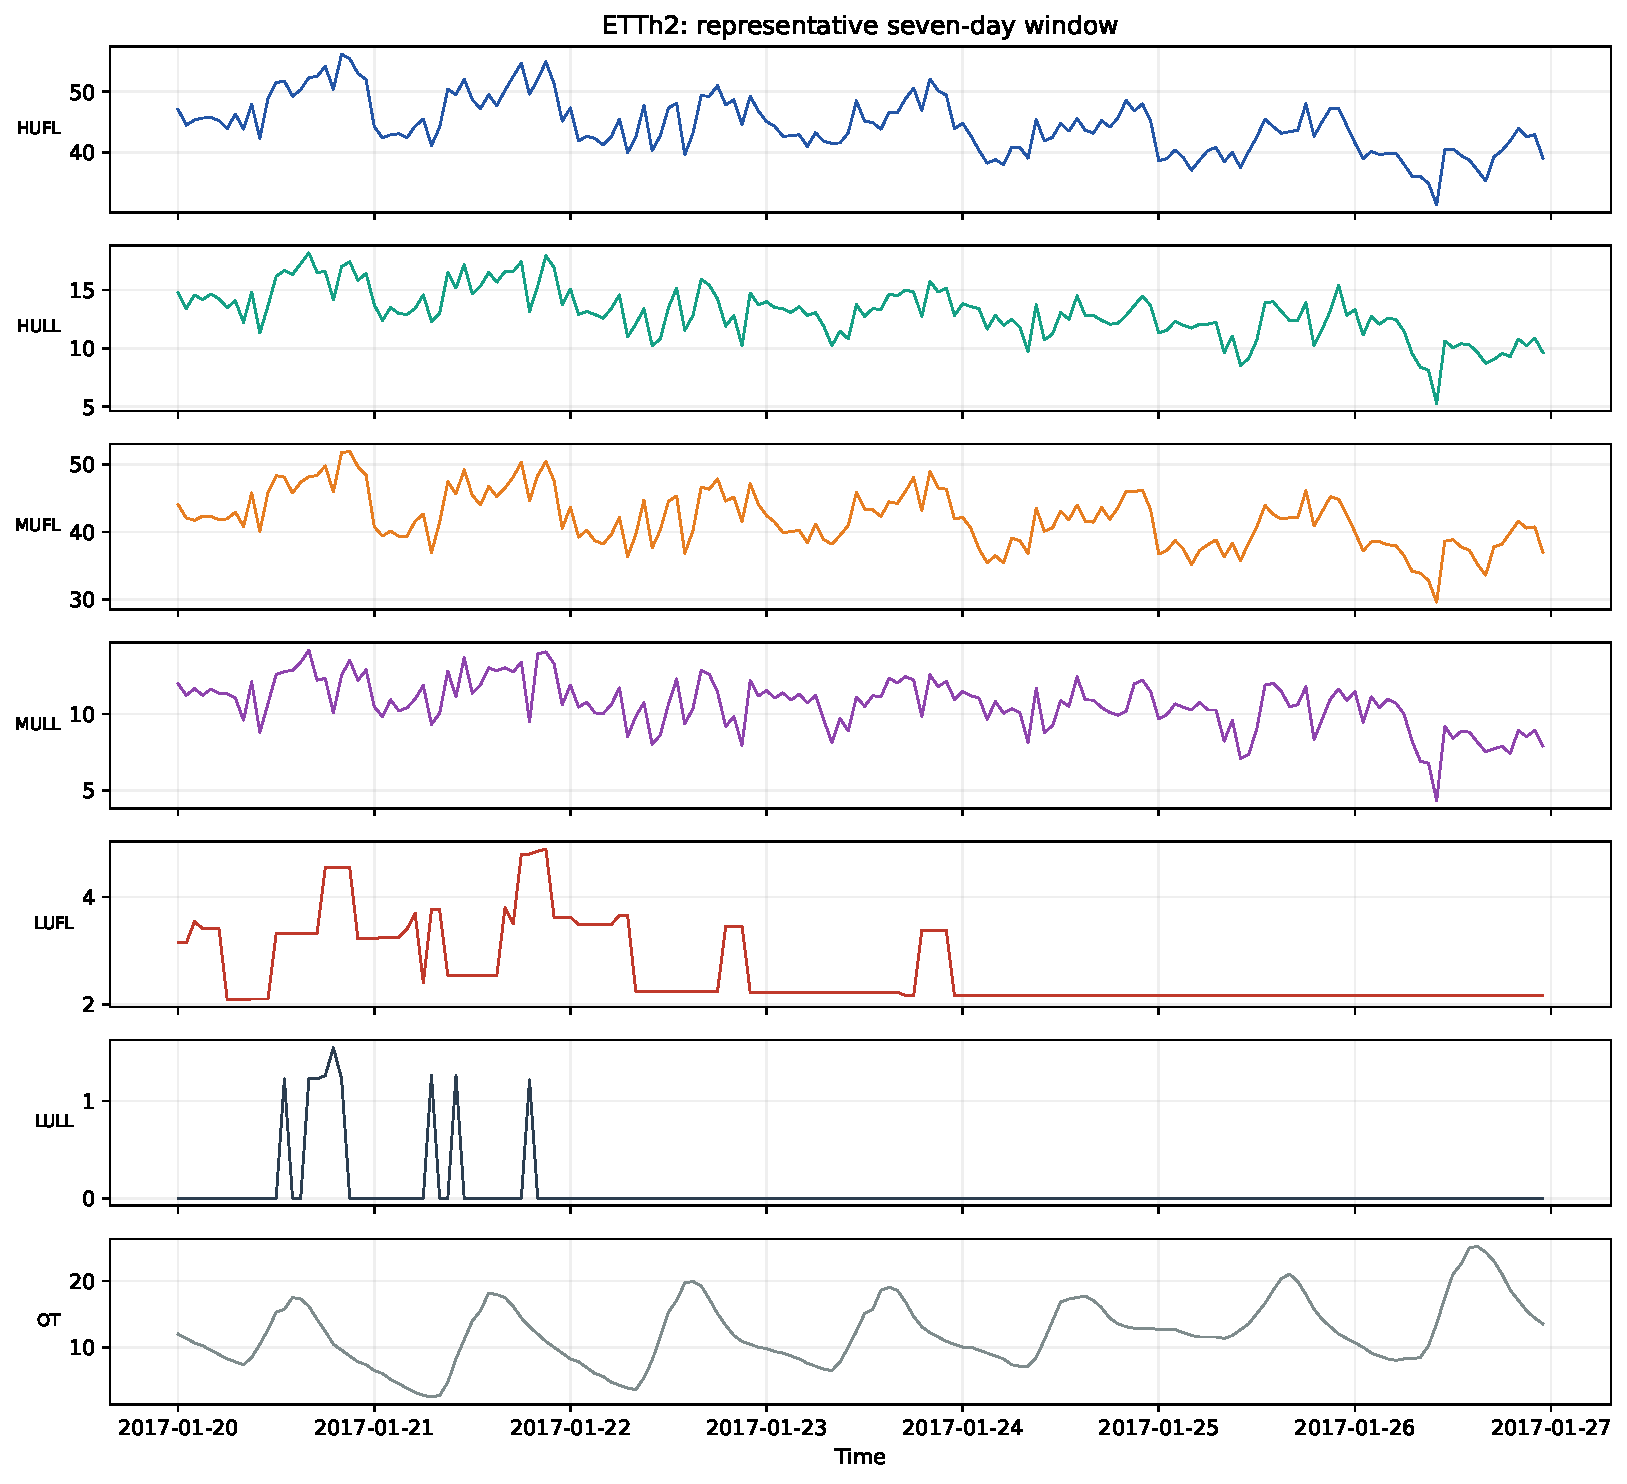
\includegraphics[width=\linewidth]{figures/ETTh2_week.pdf}\caption{Representative seven-day window.}\end{subfigure}
\caption{ETTh2 raw trajectories.}\label{fig:etth2}
\end{figure}

\subsection{ETTm1}

The local file contains 69,680 observations from 2016-07-01 00:00:00 to 2018-06-26 19:45:00 at 0.25-hour cadence. Table~\ref{tab:ettm1} reports unnormalized values.

\begin{table}[ht]
\centering\scriptsize
\caption{ETTm1 variable semantics and empirical behaviour.}\label{tab:ettm1}
\resizebox{\textwidth}{!}{%
\begin{tabular}{lllrrl}
\toprule
Variable & Meaning & Unit & Min--Max & Mean $\pm$ Std & Dominant period \\
\midrule
HUFL & High useful load & dataset load unit & -23.242--24.180 & 7.414 $\pm$ 7.083 & 24.0 h (daily) \\
HULL & High useless load & dataset load unit & -5.693--10.315 & 2.261 $\pm$ 2.041 & 24.0 h (daily) \\
MUFL & Middle useful load & dataset load unit & -26.367--18.087 & 4.322 $\pm$ 6.829 & 24.0 h (daily) \\
MULL & Middle useless load & dataset load unit & -6.041--7.853 & 0.897 $\pm$ 1.807 & 24.0 h (daily) \\
LUFL & Low useful load & dataset load unit & -1.188--8.498 & 3.083 $\pm$ 1.174 & 12.0 h (sub-daily) \\
LULL & Low useless load & dataset load unit & -1.371--3.046 & 0.858 $\pm$ 0.600 & 1161.3 h (long-cycle (48.4 d)) \\
OT & Transformer oil temperature (forecast target) & degree C & -4.221--46.007 & 13.321 $\pm$ 8.565 & 24.0 h (daily) \\
\bottomrule
\end{tabular}}
\end{table}

\begin{table}[ht]
\centering\small
\caption{ETTm1 load--oil-temperature relations. Level correlation is contemporaneous; lag is selected on first differences.}\label{tab:ettm1lags}
\begin{tabular}{lrrlr}
\toprule
Load & Level $\rho$ & Best lag (h) & Direction & Change $\rho$ \\
\midrule
HUFL & 0.061 & 1.8 & load leads & -0.040 \\
HULL & 0.225 & -27.2 & load lags & -0.021 \\
MUFL & 0.052 & 1.8 & load leads & -0.039 \\
MULL & 0.220 & -28.0 & load lags & -0.023 \\
LUFL & 0.120 & -22.2 & load lags & -0.022 \\
LULL & 0.069 & -14.8 & load lags & 0.014 \\
\bottomrule
\end{tabular}
\end{table}

\begin{figure}[ht]
\centering
\begin{subfigure}{.49\textwidth}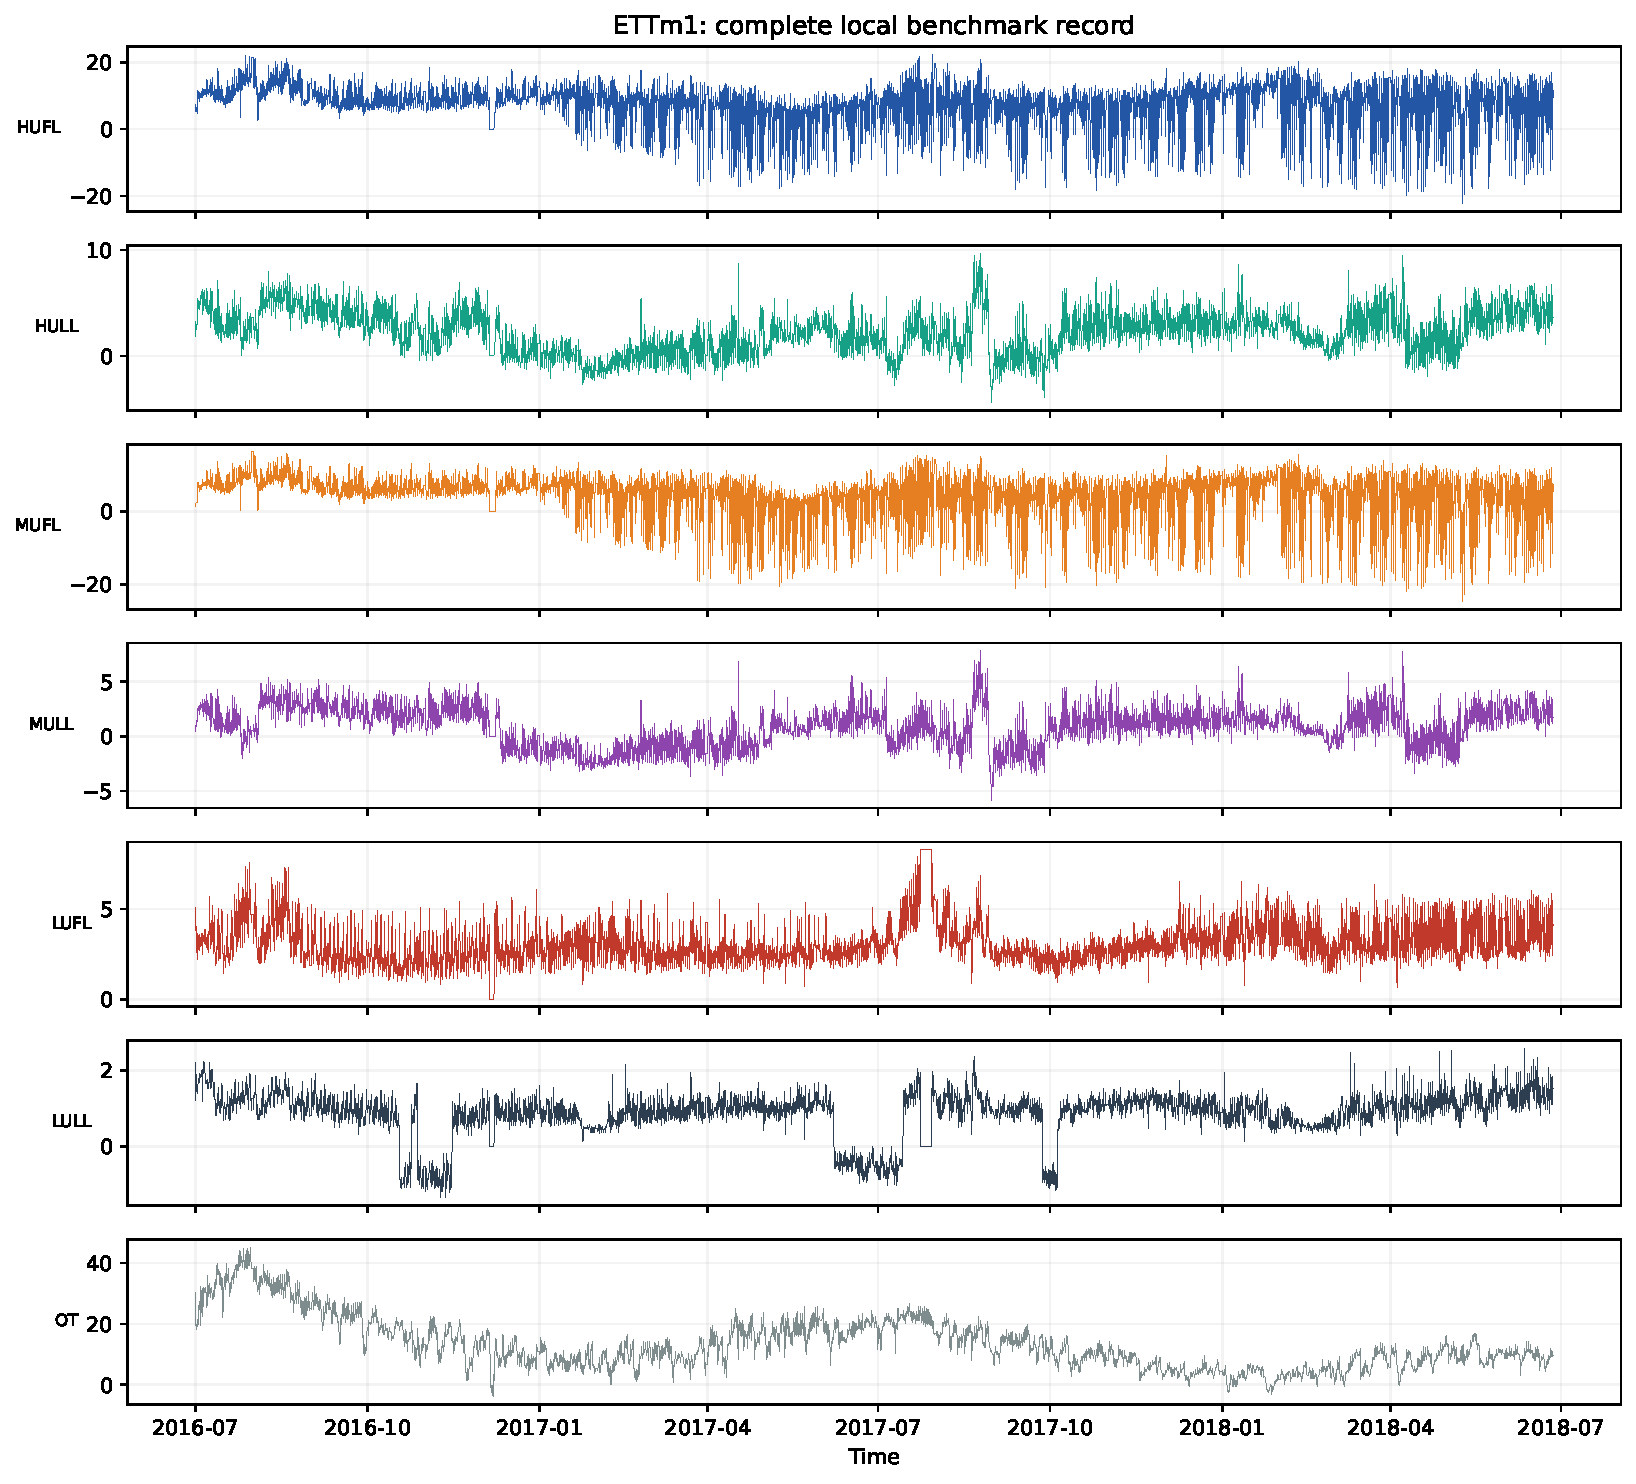
\includegraphics[width=\linewidth]{figures/ETTm1_full.pdf}\caption{Complete record.}\end{subfigure}
\begin{subfigure}{.49\textwidth}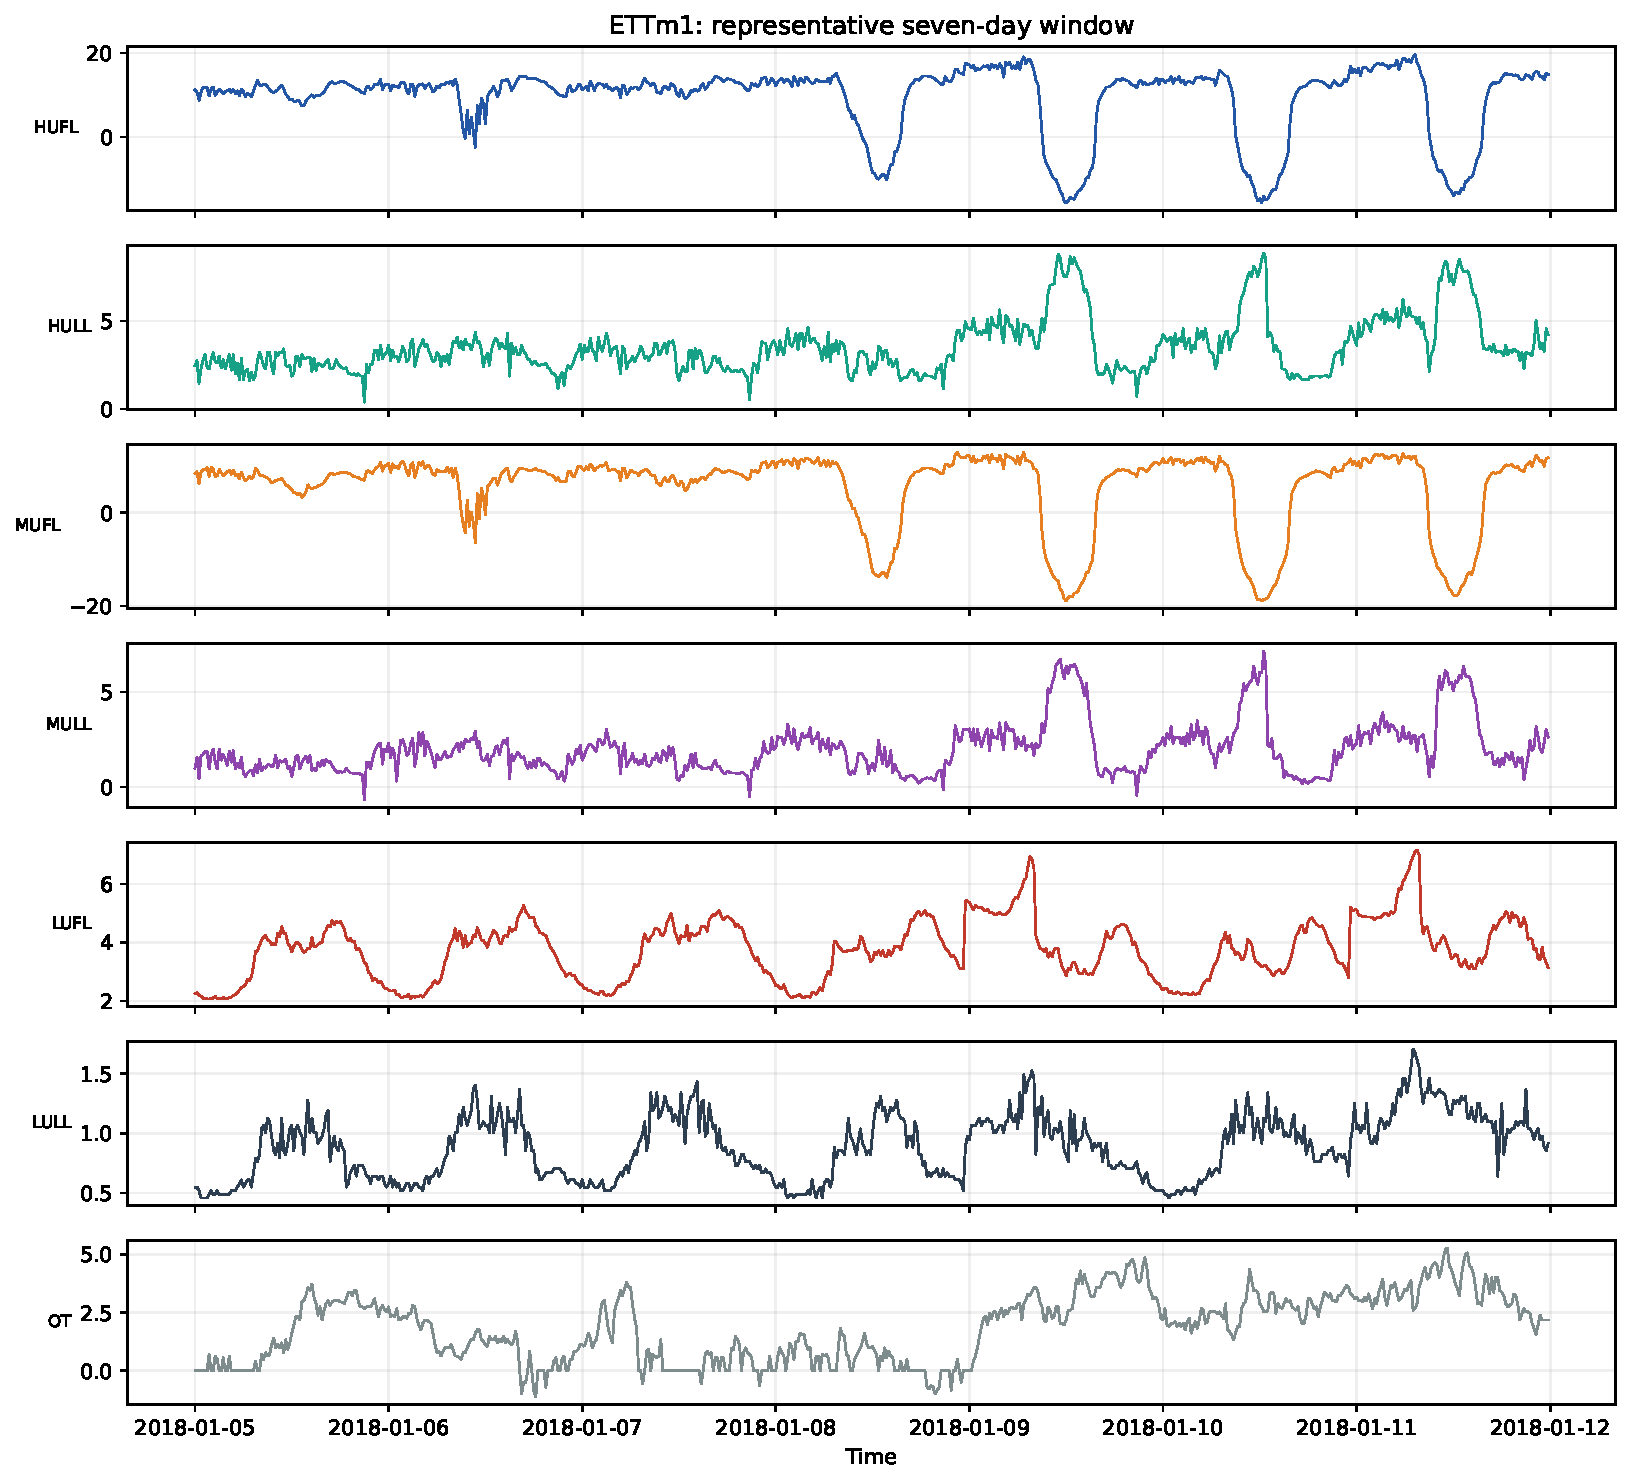
\includegraphics[width=\linewidth]{figures/ETTm1_week.pdf}\caption{Representative seven-day window.}\end{subfigure}
\caption{ETTm1 raw trajectories.}\label{fig:ettm1}
\end{figure}

\subsection{ETTm2}

The local file contains 69,680 observations from 2016-07-01 00:00:00 to 2018-06-26 19:45:00 at 0.25-hour cadence. Table~\ref{tab:ettm2} reports unnormalized values.

\begin{table}[ht]
\centering\scriptsize
\caption{ETTm2 variable semantics and empirical behaviour.}\label{tab:ettm2}
\resizebox{\textwidth}{!}{%
\begin{tabular}{lllrrl}
\toprule
Variable & Meaning & Unit & Min--Max & Mean $\pm$ Std & Dominant period \\
\midrule
HUFL & High useful load & dataset load unit & 0.000--107.893 & 37.219 $\pm$ 10.243 & 24.0 h (daily) \\
HULL & High useless load & dataset load unit & -29.319--36.439 & 8.554 $\pm$ 6.031 & 967.8 h (long-cycle (40.3 d)) \\
MUFL & Middle useful load & dataset load unit & 10.427--93.230 & 43.861 $\pm$ 13.062 & 24.0 h (daily) \\
MULL & Middle useless load & dataset load unit & -6.648--29.808 & 8.340 $\pm$ 4.369 & 483.9 h (long-cycle (20.2 d)) \\
LUFL & Low useful load & dataset load unit & -14.617--17.218 & -3.431 $\pm$ 6.154 & 791.8 h (long-cycle (33.0 d)) \\
LULL & Low useless load & dataset load unit & -31.462--3.731 & -2.085 $\pm$ 6.014 & 1340.0 h (long-cycle (55.8 d)) \\
OT & Transformer oil temperature (forecast target) & degree C & -2.647--58.877 & 26.610 $\pm$ 11.886 & 24.0 h (daily) \\
\bottomrule
\end{tabular}}
\end{table}

\begin{table}[ht]
\centering\small
\caption{ETTm2 load--oil-temperature relations. Level correlation is contemporaneous; lag is selected on first differences.}\label{tab:ettm2lags}
\begin{tabular}{lrrlr}
\toprule
Load & Level $\rho$ & Best lag (h) & Direction & Change $\rho$ \\
\midrule
HUFL & 0.034 & 0.0 & synchronous & 0.065 \\
HULL & 0.337 & 0.0 & synchronous & 0.052 \\
MUFL & 0.194 & 10.5 & load leads & -0.060 \\
MULL & 0.495 & 0.0 & synchronous & 0.054 \\
LUFL & -0.144 & -46.0 & load lags & -0.031 \\
LULL & -0.113 & 18.0 & load leads & 0.019 \\
\bottomrule
\end{tabular}
\end{table}

\begin{figure}[ht]
\centering
\begin{subfigure}{.49\textwidth}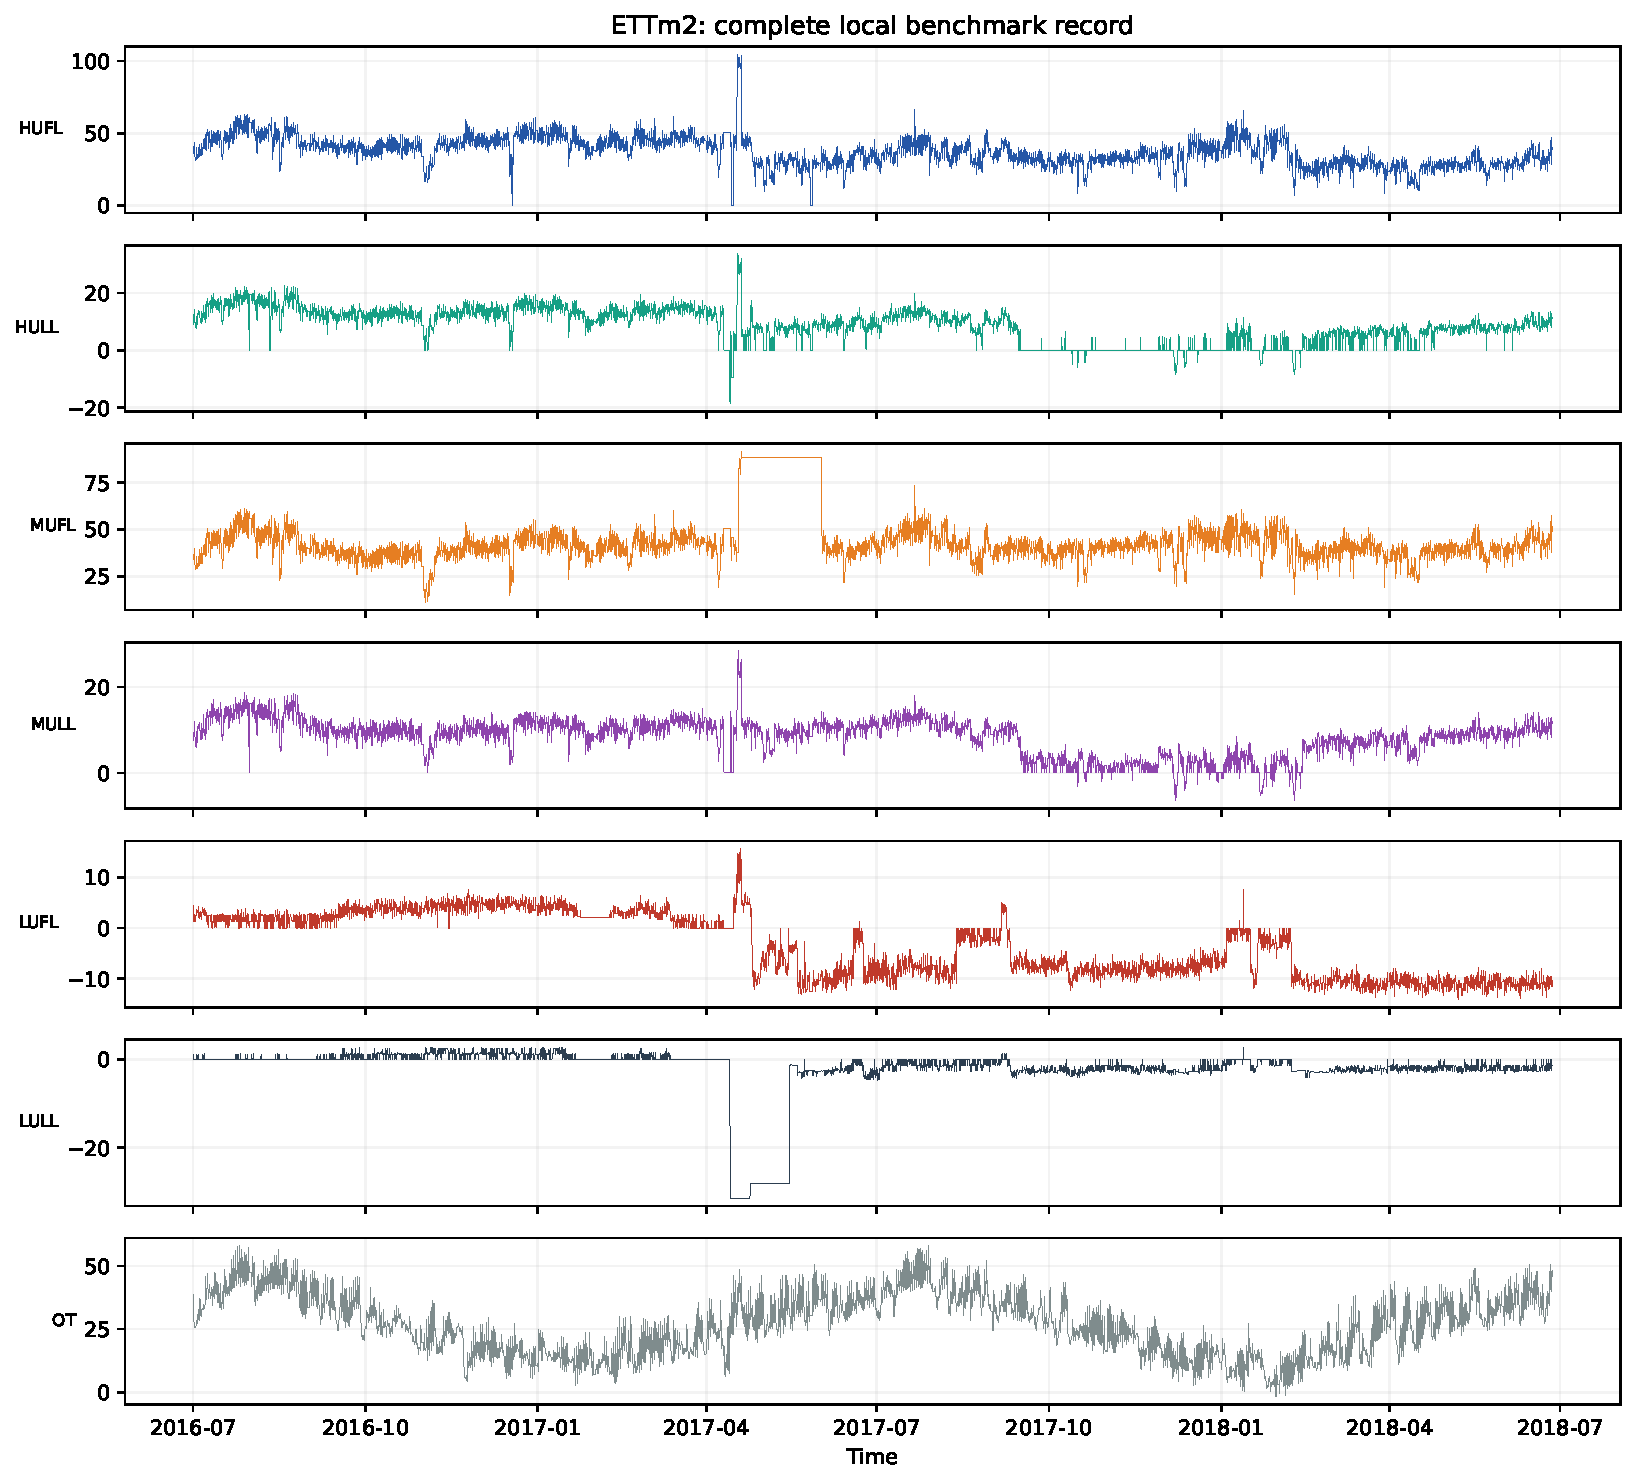
\includegraphics[width=\linewidth]{figures/ETTm2_full.pdf}\caption{Complete record.}\end{subfigure}
\begin{subfigure}{.49\textwidth}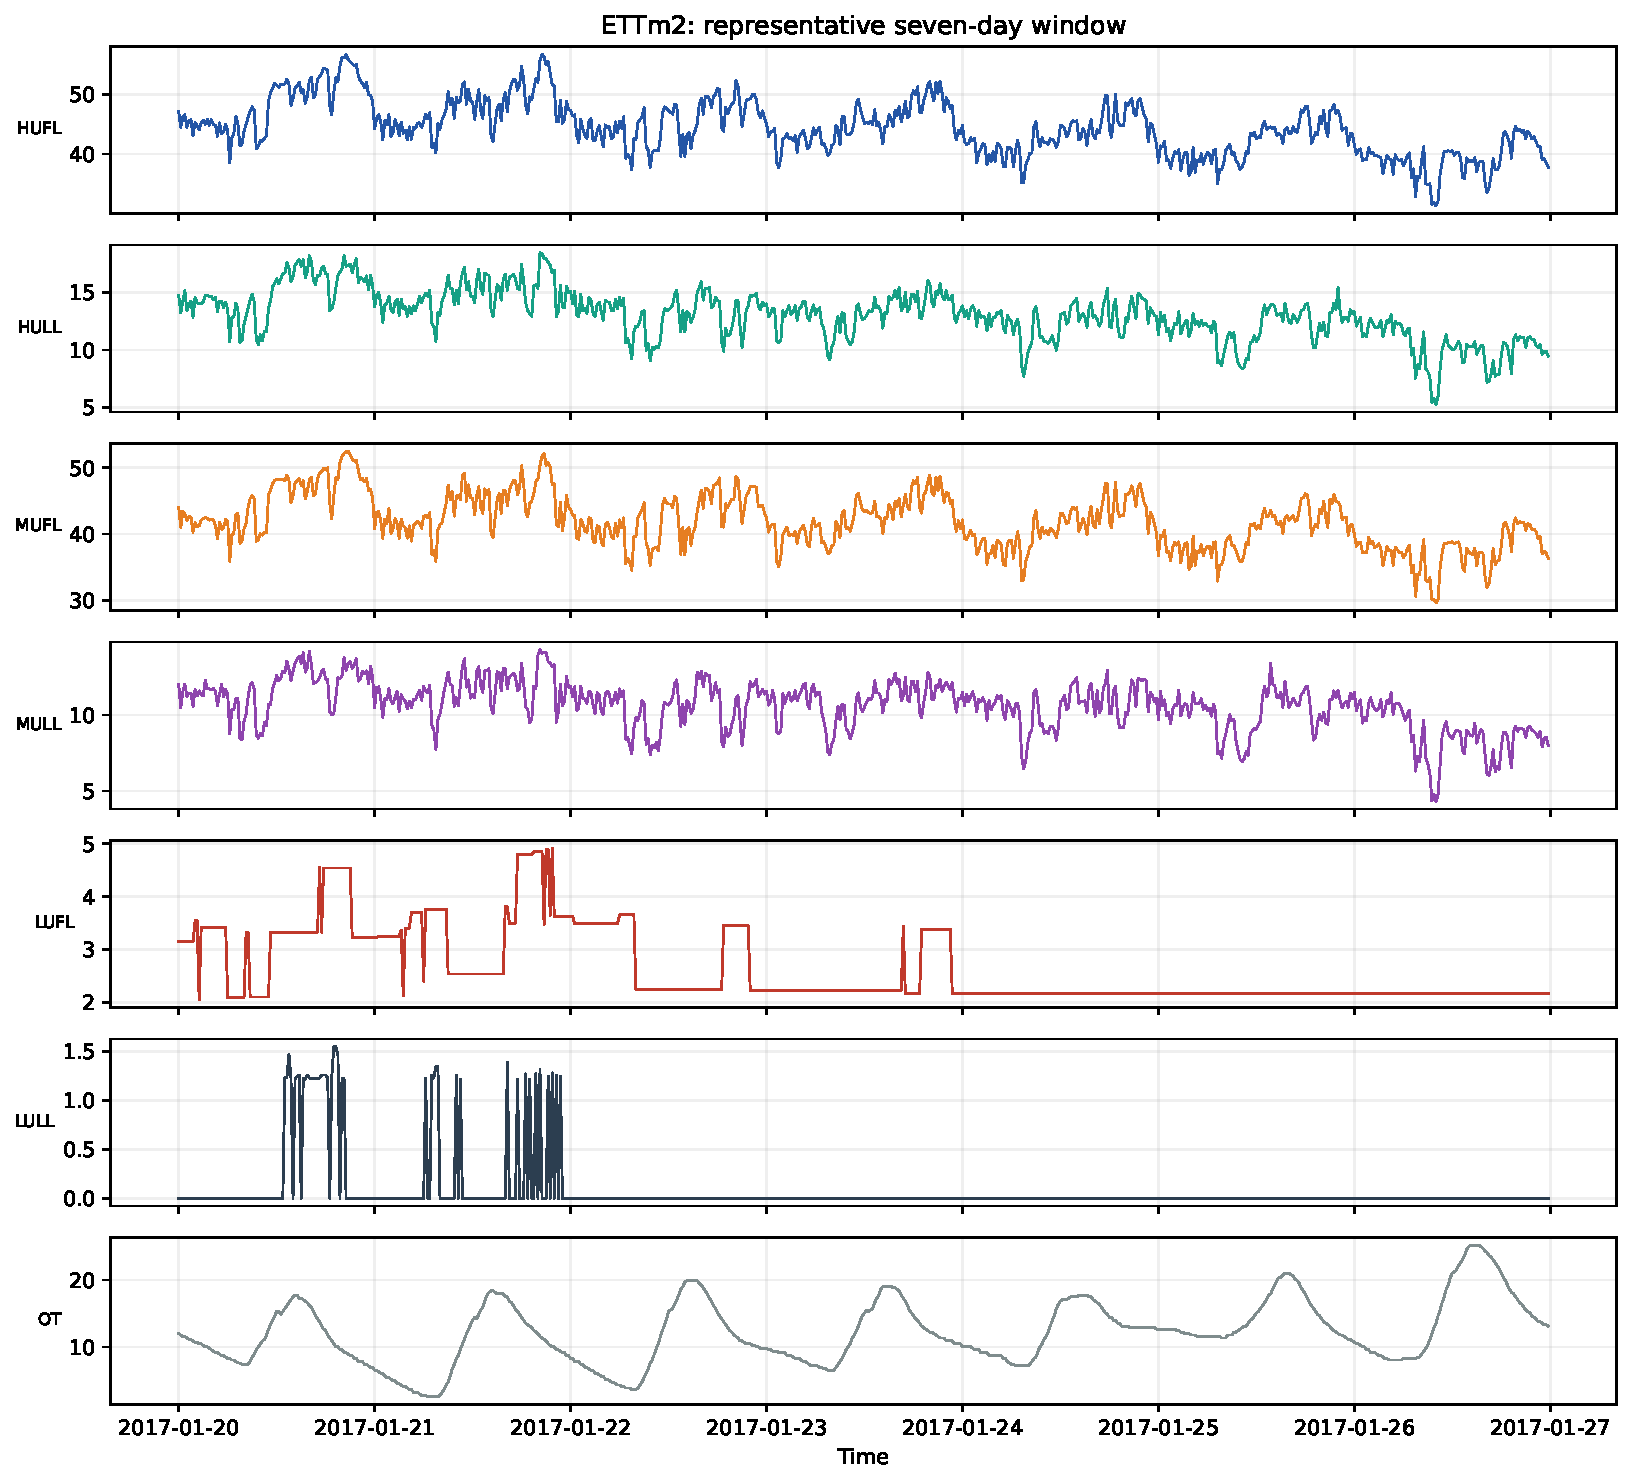
\includegraphics[width=\linewidth]{figures/ETTm2_week.pdf}\caption{Representative seven-day window.}\end{subfigure}
\caption{ETTm2 raw trajectories.}\label{fig:ettm2}
\end{figure}

\subsection{Cross-station and sampling comparison}
The hourly and 15-minute versions of a station have closely matched marginal distributions, as expected from alternate sampling of the same physical system: station 1 oil temperature has mean 13.325 (ETTh1) versus 13.321 (ETTm1), while station 2 has mean 26.609 in both resolutions. The larger contrast is between stations. Station 2 oil temperature spans approximately $-2.65$ to $58.88\,^{\circ}$C, compared with $-4.22$ to $46.01\,^{\circ}$C at station 1; its HUFL and MUFL also reach 107.893 and 93.230, far above station 1. Daily load periodicity and smoother oil-temperature motion recur across the four files, but several station-2 channels are dominated by slower multiweek spectral peaks. Lead/lag signs should be read as predictive timing, not thermal causality: differencing suppresses common slow trends, but weather, dispatch, and controller state remain unobserved confounders.

\paragraph{Modelling implication.}
ETT is low-dimensional but not univariate. A useful model should preserve sharp daily load changes while continuing the smoother thermal state, and it should not assume that one station's normalization or cross-channel coupling transfers unchanged to the other. The weak-to-moderate change correlations also argue against treating any single load as a deterministic driver of oil temperature.


\section{Weather}

The local Weather panel contains 52,696 ten-minute observations from 2020-01-01 00:10:00 to 2021-01-01 00:00:00 and 21 variables. We excluded 81 occurrences of the source missing sentinel $-9999$ before every statistic. Variables are grouped by physical role; CO2 is retained as a separate atmospheric-composition group.

\scriptsize
\setlength{\tabcolsep}{3pt}
\begin{longtable}{@{}p{.09\textwidth}p{.19\textwidth}p{.10\textwidth}p{.13\textwidth}rrp{.20\textwidth}@{}}
\caption{Weather variable dictionary and statistics after excluding $-9999$ sentinels.}\label{tab:weather}\\
\toprule
Variable & Meaning & Unit & Group & Min--Max & Mean $\pm$ Std & Main pattern \\
\midrule\endfirsthead
\toprule
Variable & Meaning & Unit & Group & Min--Max & Mean $\pm$ Std & Main pattern \\
\midrule\endhead
p (mbar) & Air pressure & mbar & pressure/density & 955.580--1020.070 & 989.989 $\pm$ 9.207 & smooth/moderate; long-cycle (52.3 d) \\
T (degC) & Air temperature & $^\circ$C & temperature & -6.440--34.800 & 10.818 $\pm$ 7.469 & smooth/moderate; daily \\
Tpot (K) & Potential temperature & K & temperature & 266.190--309.130 & 284.797 $\pm$ 7.617 & smooth/moderate; daily \\
Tdew (degC) & Dew-point temperature & $^\circ$C & temperature & -13.810--20.500 & 5.409 $\pm$ 5.957 & smooth/moderate; long-cycle (52.3 d) \\
rh (\%) & Relative humidity & \% & humidity & 21.160--100.000 & 72.487 $\pm$ 19.230 & smooth/moderate; daily \\
VPmax (mbar) & Saturation vapor pressure & mbar & humidity & 3.770--55.670 & 14.487 $\pm$ 7.633 & smooth/moderate; daily \\
VPact (mbar) & Actual vapor pressure & mbar & humidity & 2.090--24.160 & 9.677 $\pm$ 4.023 & smooth/moderate; long-cycle (52.3 d) \\
VPdef (mbar) & Vapor-pressure deficit & mbar & humidity & 0.000--42.100 & 4.810 $\pm$ 5.539 & smooth/moderate; daily \\
sh (g/kg) & Specific humidity & g\,kg$^{-1}$ & humidity & 1.300--15.400 & 6.111 $\pm$ 2.562 & smooth/moderate; long-cycle (52.3 d) \\
H2OC (mmol/mol) & Water-vapor concentration & mmol\,mol$^{-1}$ & humidity & 2.090--24.530 & 9.782 $\pm$ 4.083 & smooth/moderate; long-cycle (52.3 d) \\
rho (g/m**3) & Air density & g\,m$^{-3}$ & pressure/density & 1107.380--1318.520 & 1210.883 $\pm$ 36.430 & smooth/moderate; daily \\
wv (m/s) & Mean wind speed & m\,s$^{-1}$ & wind & 0.080--13.770 & 2.186 $\pm$ 1.602 & gusty with a daily spectral component \\
max. wv (m/s) & Maximum wind speed & m\,s$^{-1}$ & wind & 0.000--22.900 & 3.633 $\pm$ 2.462 & gusty with a daily spectral component \\
wd (deg) & Wind direction & degree & wind & 0.000--360.000 & 176.850 $\pm$ 81.194 & circular and abrupt; Euclidean roughness is misleading \\
rain (mm) & Precipitation amount & mm & precipitation/radiation & 0.000--11.200 & 0.012 $\pm$ 0.123 & sharp/intermittent precipitation events \\
raining (s) & Duration of precipitation in interval & s & precipitation/radiation & 0.000--600.000 & 25.907 $\pm$ 111.502 & sharp/intermittent precipitation events \\
SWDR & Short-wave downward radiation & W\,m$^{-2}$ & precipitation/radiation & 0.000--1115.290 & 131.332 $\pm$ 215.733 & smooth daily daylight envelope with night zeros \\
PAR & Photosynthetically active radiation & $\mu$mol\,m$^{-2}$\,s$^{-1}$ & precipitation/radiation & 0.000--2131.760 & 259.863 $\pm$ 422.783 & smooth daily daylight envelope with night zeros \\
max. PAR & Maximum photosynthetically active radiation & $\mu$mol\,m$^{-2}$\,s$^{-1}$ & precipitation/radiation & 0.000--2498.940 & 314.473 $\pm$ 514.270 & smooth daily daylight envelope with night zeros \\
Tlog (degC) & Data-logger internal temperature & $^\circ$C & temperature & 6.900--49.090 & 21.515 $\pm$ 7.791 & smooth/moderate; daily \\
OT & Ambient CO$_2$ concentration (locally renamed from source CO2 channel) & ppm & atmospheric composition & 305.500--524.200 & 427.692 $\pm$ 18.700 & smooth/moderate; daily \\
\bottomrule
\end{longtable}
\normalsize

\begin{table}[ht]\centering\small
\caption{Within-group Weather co-movement and roughness.}\label{tab:weather-groups}
\begin{tabular}{lrrr}
\toprule
Group & Variables & Median within-group $\rho$ & Median roughness \\
\midrule
pressure/density & 2 & 0.437 & 0.020 \\
temperature & 4 & 0.881 & 0.034 \\
humidity & 6 & 0.256 & 0.039 \\
wind & 3 & 0.001 & 0.379 \\
precipitation/radiation & 5 & -0.042 & 0.277 \\
atmospheric composition & 1 & -- & 0.143 \\
\bottomrule
\end{tabular}
\end{table}

\begin{figure}[ht]
\centering
\begin{subfigure}{.62\textwidth}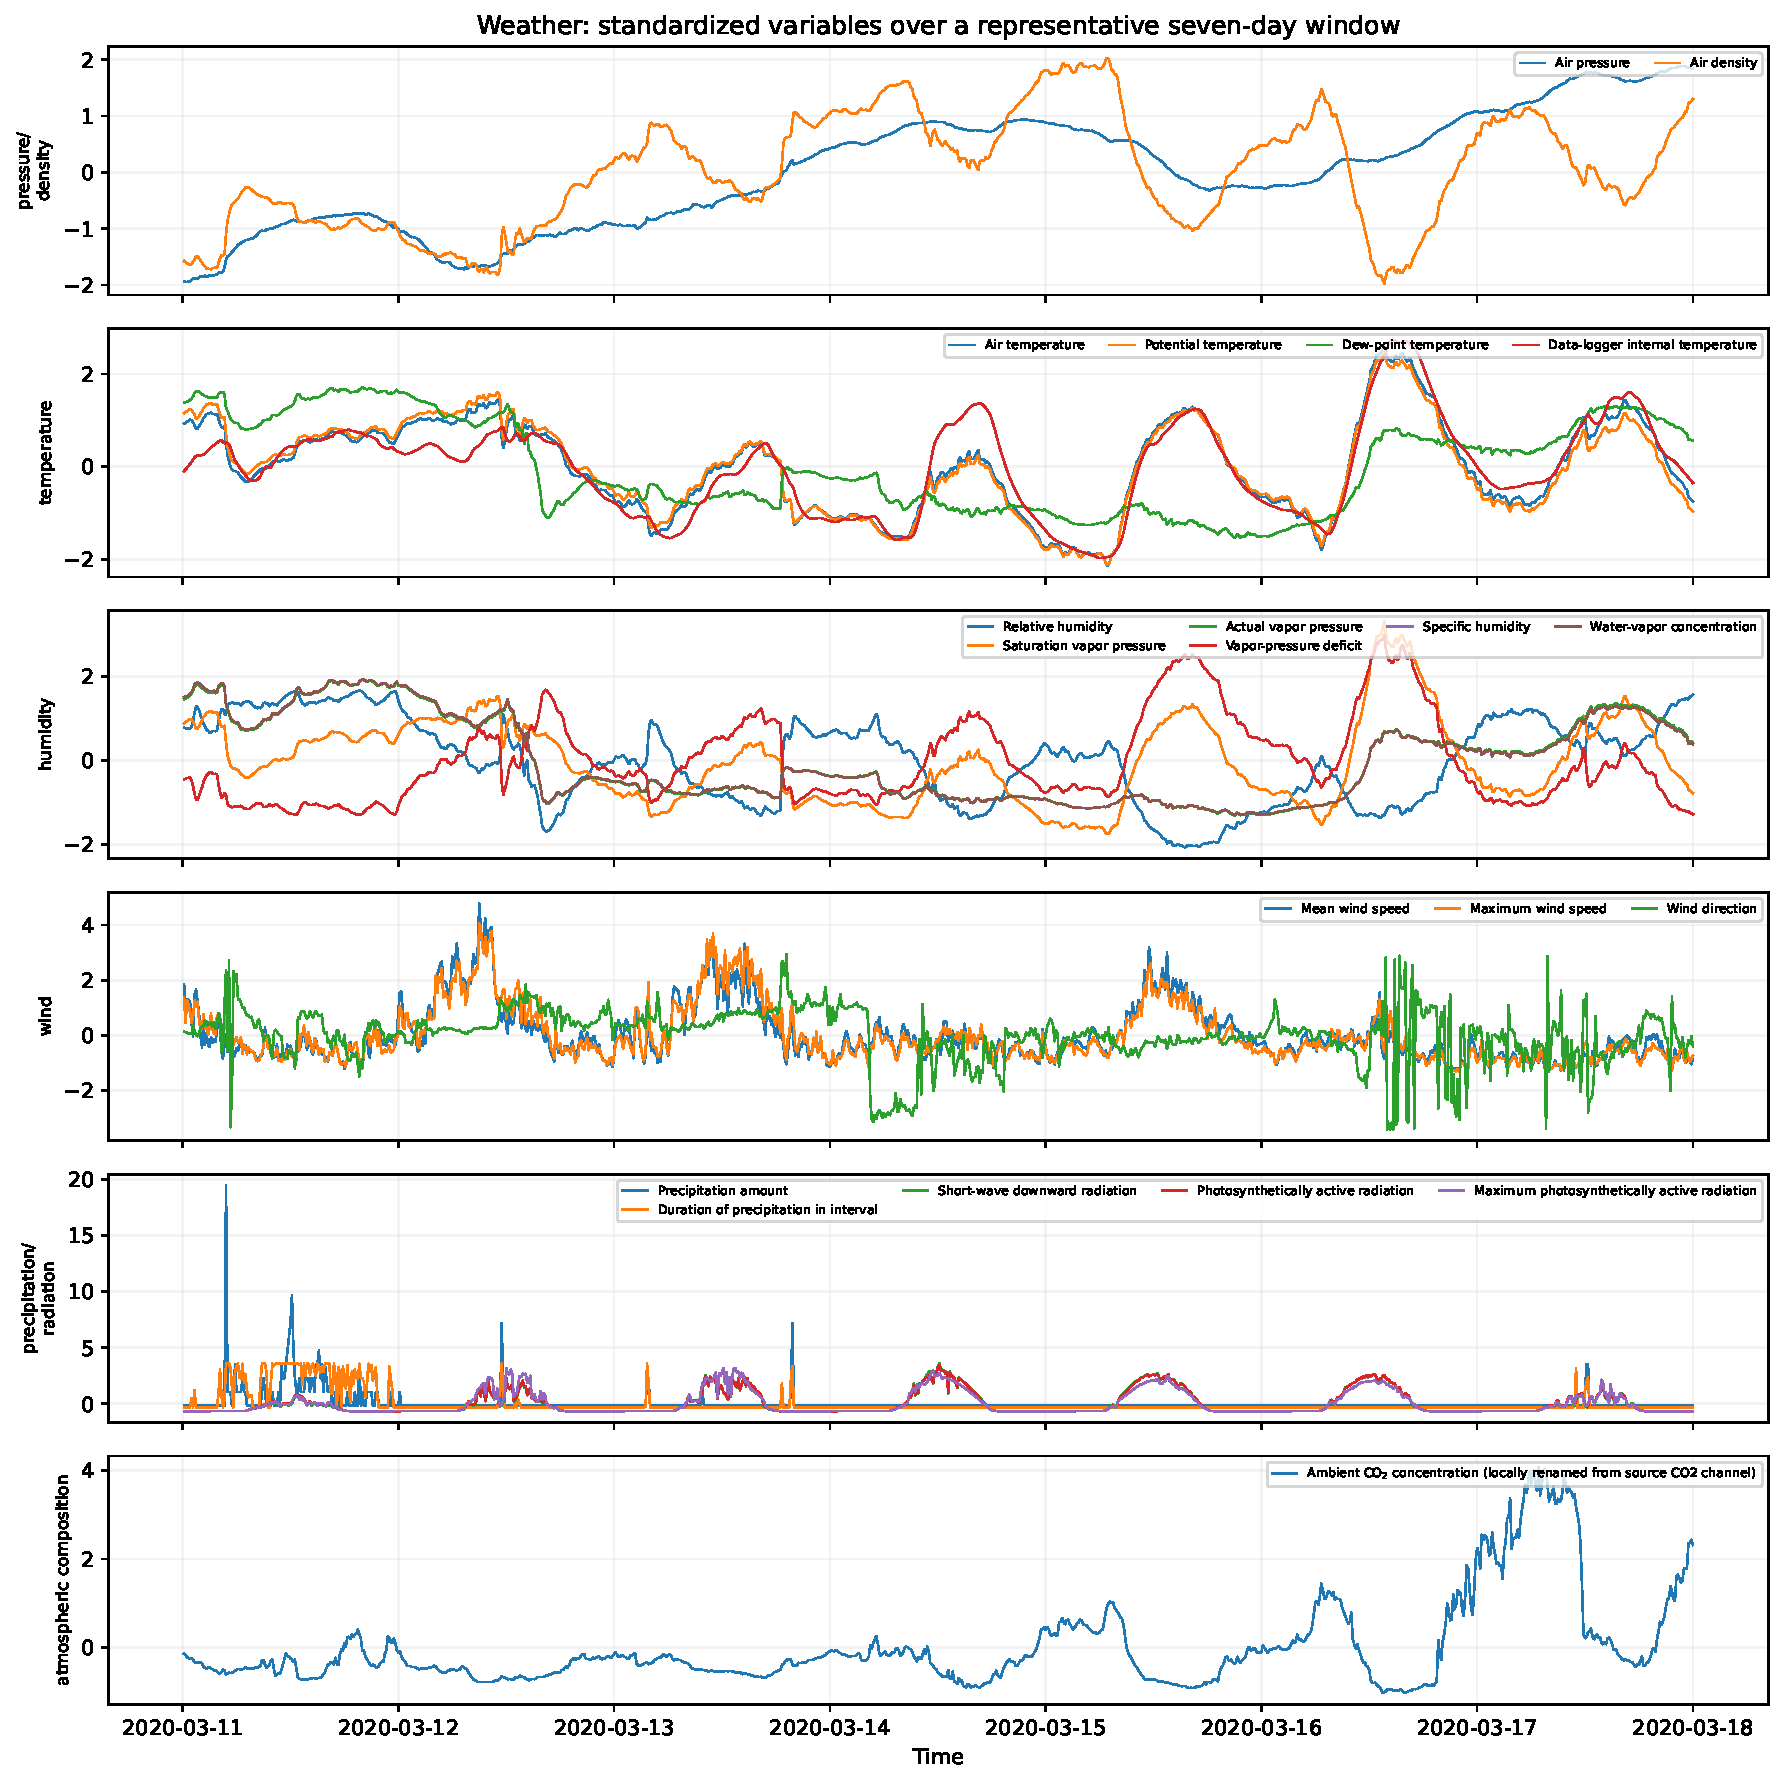
\includegraphics[width=\linewidth]{figures/Weather_groups_week.pdf}\caption{Standardized group trajectories.}\end{subfigure}
\begin{subfigure}{.36\textwidth}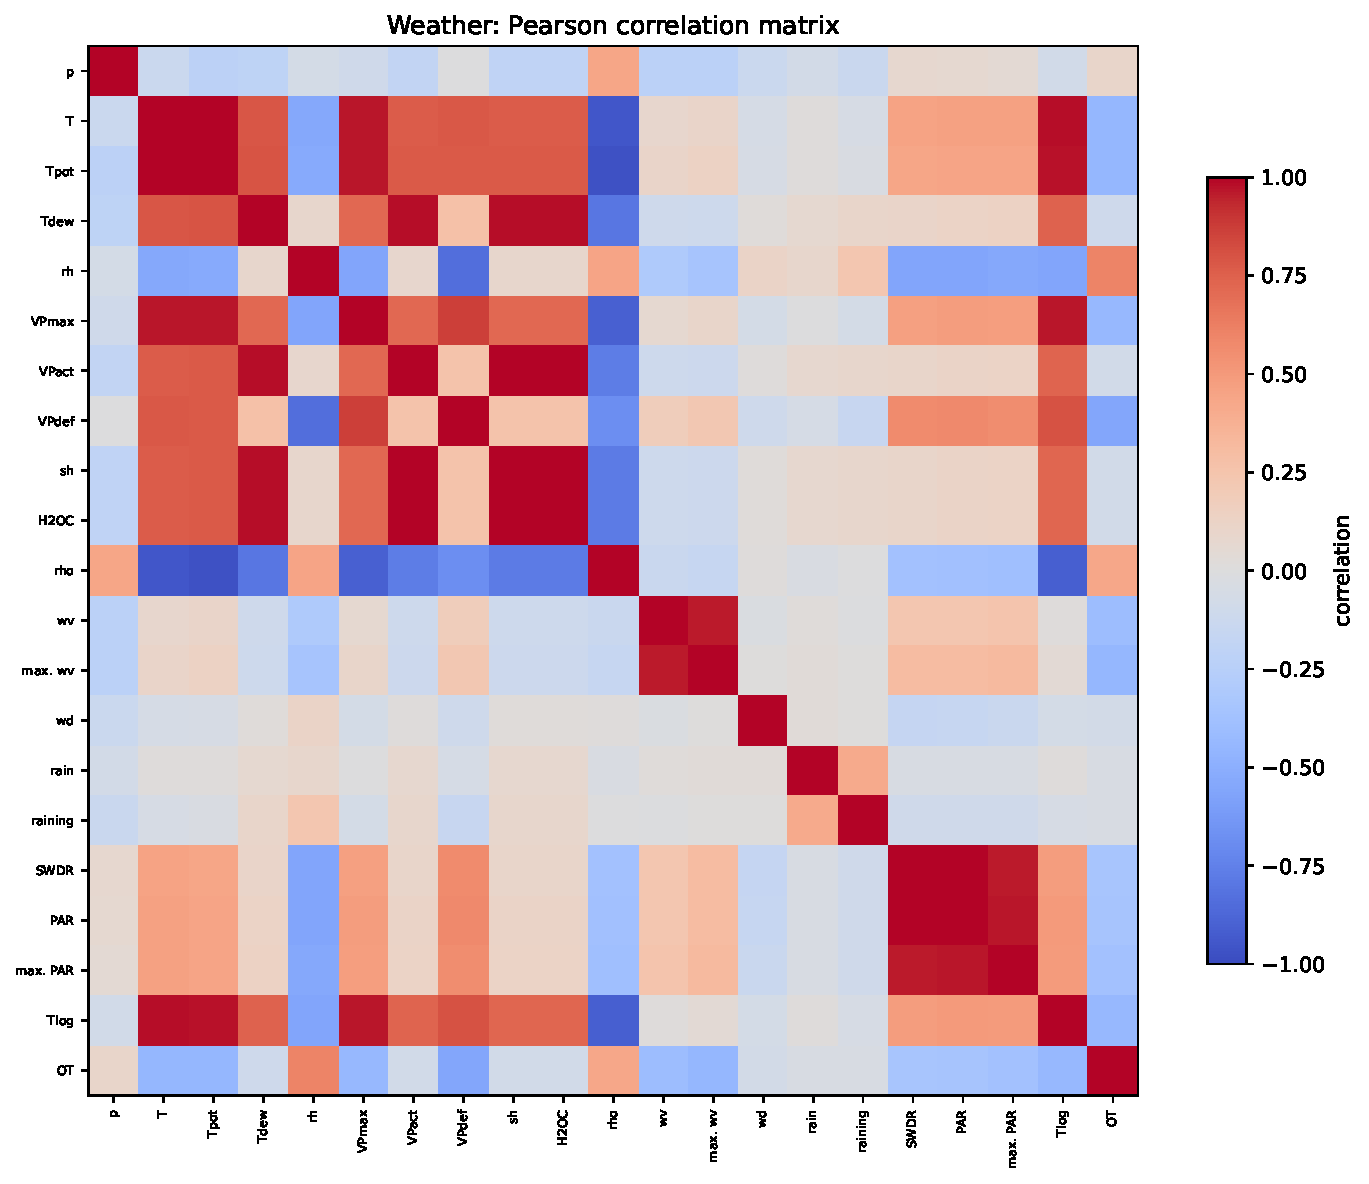
\includegraphics[width=\linewidth]{figures/Weather_correlation.pdf}\caption{Variable correlation.}\end{subfigure}
\caption{Weather behaviour and co-movement. Standardization is used only for visualization.}\label{fig:weather}
\end{figure}

Temperature, potential temperature, dew point, and logger temperature are smooth state variables with strong common motion. Vapor-pressure and humidity variables are physically coupled transformations and consequently move together, although relative humidity and vapor-pressure deficit often oppose one another. Wind direction is circular and should not be treated as an ordinary Euclidean scalar; sine/cosine encoding is preferable. Rain duration and amount are sparse and sharp, while radiation has a strong daylight envelope. These distinctions explain why one shared smoothness prior is inappropriate.

\paragraph{Modelling implication.}
Weather requires heterogeneous observation models: smooth continuation for thermodynamic state, bounded/circular treatment for wind direction, and intermittent-event capacity for rain and gusts. High within-group correlation also means that evaluating cross-variable modules solely on aggregate error can hide redundancy; group-wise errors are a useful diagnostic.


\section{Electricity}

Each channel is an anonymized electricity client. The source archive records quarter-hour power in kW; the local benchmark is an hourly 321-channel transformation, so values below are reported in the local stored scale rather than silently converting units. The final column `OT' is anonymous client 320. The local file spans 2016-07-01 02:00:00 to 2019-07-02 01:00:00 (26,304 observations).

Using the preregistered thresholds, 0.00\% of channels are nearly constant and 3.12\% are highly volatile. The median 24-hour and 168-hour lag correlations are 0.932 and 0.918. The median correlation of anonymous channels with the local `OT' channel is 0.471; this is a panel-dependence summary, not a target-causality claim.

\begin{table}[ht]\centering\small
\caption{Electricity representative channels selected by activity-mean quantiles.}\label{tab:electricity-reps}
\begin{tabular}{llrrrl}
\toprule
Activity & Channel & Min--Max & Mean $\pm$ Std & $\rho_{24}$ & Cluster \\
\midrule
low & 125 & 0.000--295.000 & 135.455 $\pm$ 21.204 & 0.842 & irregular/high variability \\
medium & 253 & 4.000--1143.000 & 591.950 $\pm$ 184.221 & 0.938 & strongly periodic \\
high & 187 & 0.000--5956.000 & 3734.345 $\pm$ 1068.911 & 0.957 & strongly periodic \\
\bottomrule
\end{tabular}
\end{table}

\begin{table}[ht]\centering\small
\caption{Electricity data-driven behavioural clusters ($k=3$, seed 42).}\label{tab:electricity-clusters}
\begin{tabular}{lrrrrrr}
\toprule
Cluster & $n$ & Share & Median mean & Median std & $\rho_{24}$ & $\rho_{168}$ \\
\midrule
irregular/high variability & 114 & 35.5\% & 242.351 & 85.276 & 0.863 & 0.865 \\
strongly periodic & 201 & 62.6\% & 1043.704 & 378.123 & 0.949 & 0.932 \\
low activity & 6 & 1.9\% & 120.826 & 159.544 & 0.469 & 0.750 \\
\bottomrule
\end{tabular}
\end{table}

\begin{figure}[ht]\centering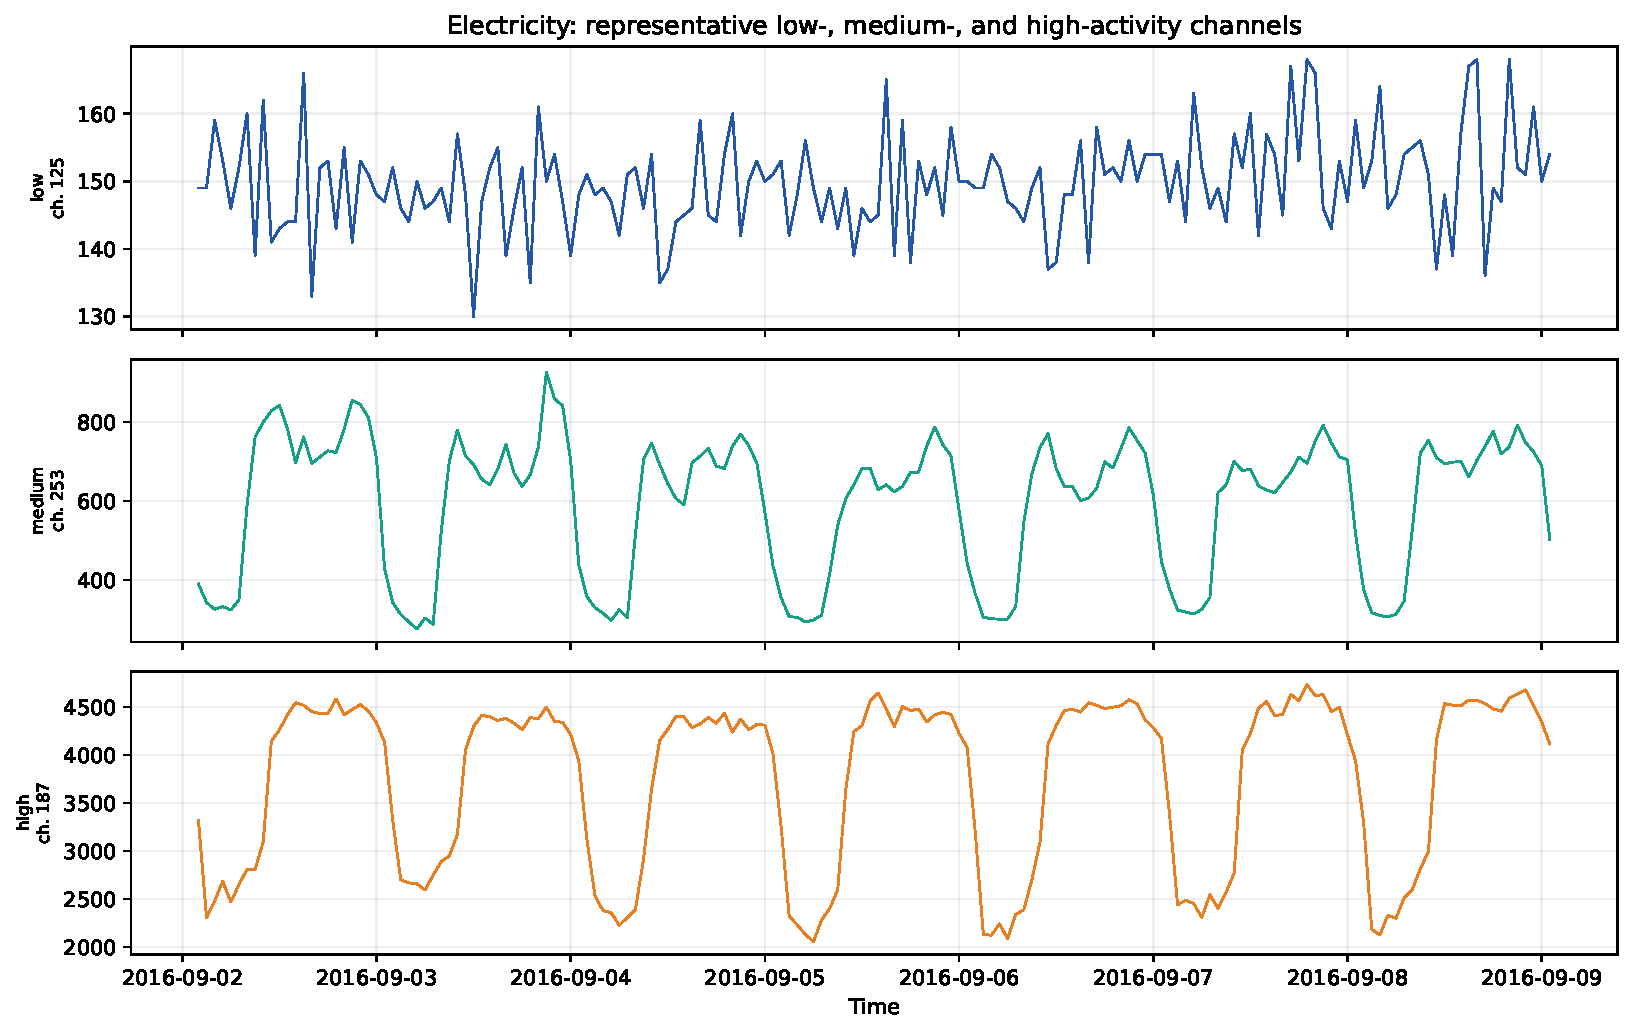
\includegraphics[width=.9\linewidth]{figures/Electricity_representatives.pdf}\caption{Electricity representative raw channels.}\label{fig:electricity}
\end{figure}

\paragraph{Modelling implication.} Client scale, zero inflation, and periodicity vary substantially. Per-channel normalization prevents large clients from dominating, while daily/weekly structure and cross-client factors motivate both temporal and variable-axis modelling. Anonymous IDs do not justify residential/commercial labels; the clusters are behavioural only.

\section{Traffic}

Each channel is an anonymized PeMS road detector's occupancy fraction, a dimensionless fraction of the sampling interval during which the detector is occupied. The local file is hourly with 862 detectors. The final column `OT' is anonymous detector 861. The local file spans 2016-07-01 02:00:00 to 2018-07-02 01:00:00 (17,544 observations).

Using the preregistered thresholds, 0.00\% of channels are nearly constant and 0.70\% are highly volatile. The median 24-hour and 168-hour lag correlations are 0.753 and 0.826. The median correlation of anonymous channels with the local `OT' channel is 0.691; this is a panel-dependence summary, not a target-causality claim.

\begin{table}[ht]\centering\small
\caption{Traffic representative channels selected by activity-mean quantiles.}\label{tab:traffic-reps}
\begin{tabular}{llrrrl}
\toprule
Activity & Channel & Min--Max & Mean $\pm$ Std & $\rho_{24}$ & Cluster \\
\midrule
low & 642 & 0.000--0.310 & 0.033 $\pm$ 0.035 & 0.767 & strongly periodic \\
medium & 818 & 0.000--0.303 & 0.054 $\pm$ 0.029 & 0.809 & strongly periodic \\
high & 196 & 0.000--0.534 & 0.082 $\pm$ 0.063 & 0.657 & irregular/high variability \\
\bottomrule
\end{tabular}
\end{table}

\begin{table}[ht]\centering\small
\caption{Traffic data-driven behavioural clusters ($k=3$, seed 42).}\label{tab:traffic-clusters}
\begin{tabular}{lrrrrrr}
\toprule
Cluster & $n$ & Share & Median mean & Median std & $\rho_{24}$ & $\rho_{168}$ \\
\midrule
strongly periodic & 350 & 40.6\% & 0.046 & 0.032 & 0.799 & 0.866 \\
irregular/high variability & 347 & 40.3\% & 0.070 & 0.060 & 0.744 & 0.821 \\
low activity & 165 & 19.1\% & 0.046 & 0.037 & 0.649 & 0.705 \\
\bottomrule
\end{tabular}
\end{table}

\begin{figure}[ht]\centering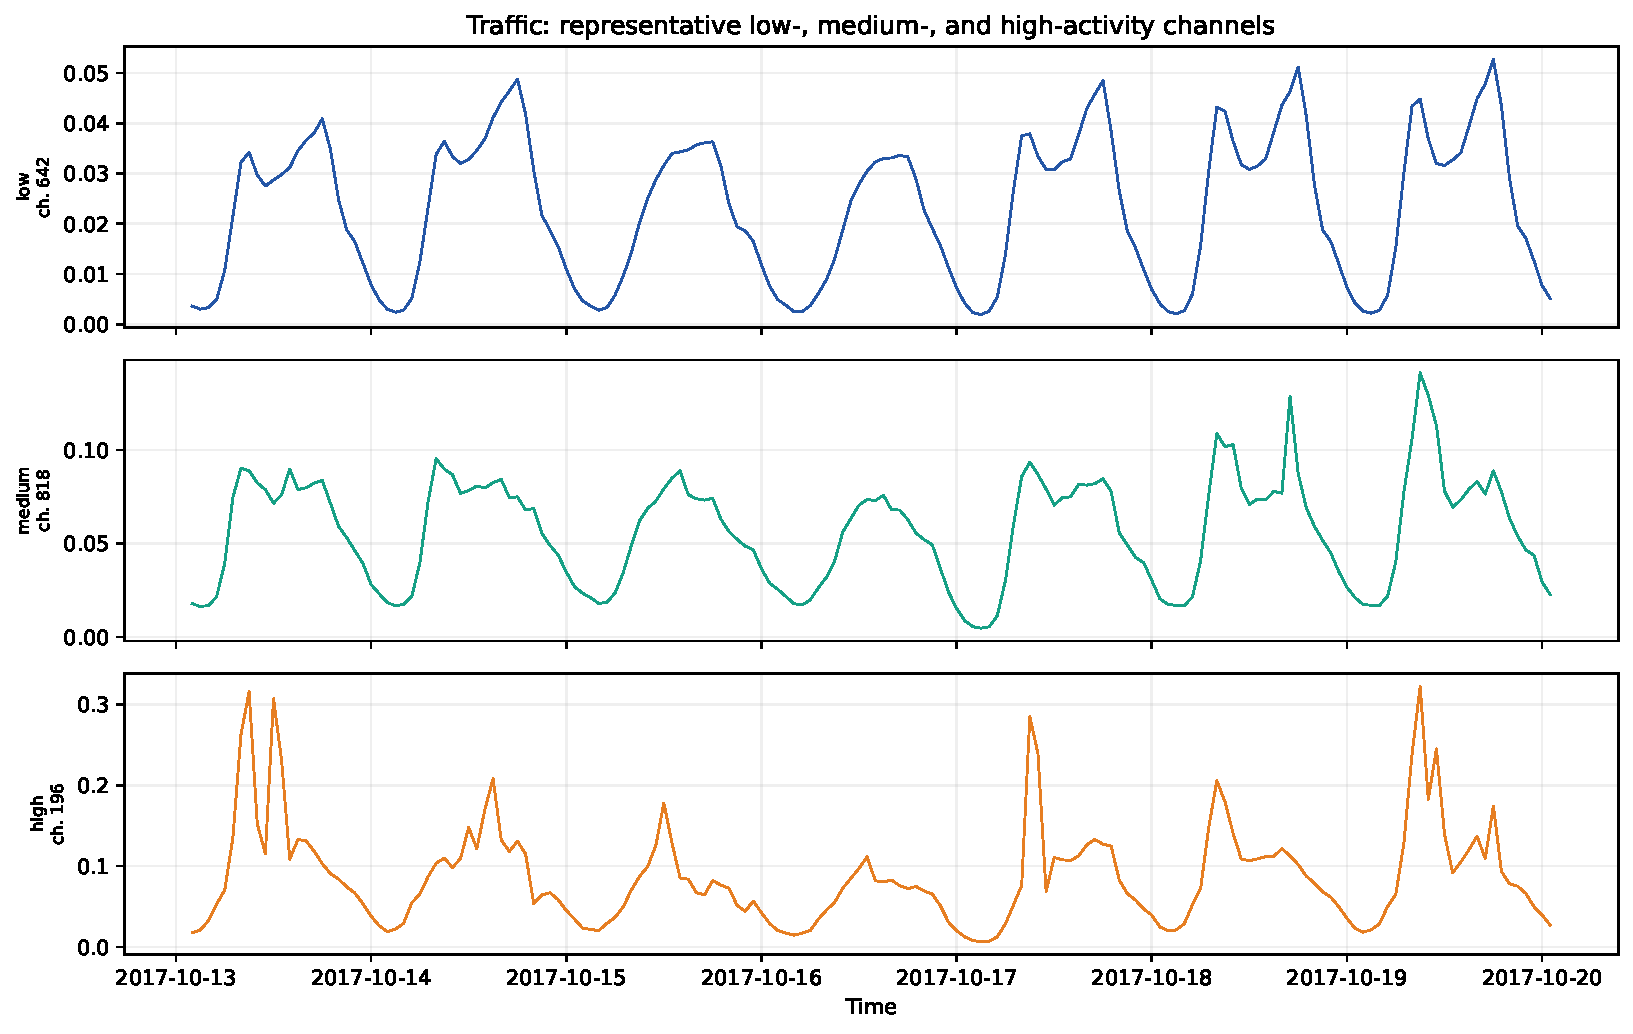
\includegraphics[width=.9\linewidth]{figures/Traffic_representatives.pdf}\caption{Traffic representative raw channels.}\label{fig:traffic}
\end{figure}

\paragraph{Modelling implication.} Occupancy is bounded, strongly periodic for many detectors, and locally irregular for others. A model should preserve detector-specific baselines while sharing congestion waves across sensors; treating all 862 channels as exchangeable ignores location-dependent behaviour.

\section{Cross-dataset conclusions}
The audit exposes three distinct geometries. ETT has only seven semantically different variables and combines daily electrical forcing with smoother transformer temperature. Weather has groups of physically coupled variables but sharply different temporal regularities. Electricity and Traffic are high-dimensional panels of repeated measurement type, where channel identity is anonymous but scale, periodicity, and volatility differ strongly. Consequently, a forecasting model should not infer ``more channels'' as ``more physical modalities'': in ETT and Weather, semantics differ by channel; in Electricity and Traffic, channels are instances of a common measurement process.

\section{Full anonymous-channel statistics}
The following appendices provide the requested per-channel ranges, means, standard deviations, daily periodicity, and cluster assignments. They are generated from the same unnormalized local files.
\subsection{Electricity channels}
\begin{longtable}{lrrrrrl}
\toprule
Channel & Min & Max & Mean & Std & $\rho_{24}$ & Cluster \\
\midrule
\endfirsthead
\toprule
Channel & Min & Max & Mean & Std & $\rho_{24}$ & Cluster \\
\midrule
\endhead
0 & 0.000 & 140.000 & 23.264 & 24.127 & 0.752 & irregular/high variability \\
1 & 0.000 & 296.000 & 112.886 & 25.553 & 0.776 & irregular/high variability \\
2 & 0.000 & 601.000 & 16.822 & 49.189 & 0.628 & irregular/high variability \\
3 & 0.000 & 1170.000 & 440.335 & 152.598 & 0.896 & irregular/high variability \\
4 & 0.000 & 547.000 & 200.537 & 69.726 & 0.878 & irregular/high variability \\
5 & 0.000 & 1984.000 & 755.035 & 249.594 & 0.908 & strongly periodic \\
6 & 0.000 & 178.000 & 25.944 & 27.392 & 0.898 & irregular/high variability \\
7 & 0.000 & 2102.000 & 1022.549 & 231.476 & 0.849 & irregular/high variability \\
8 & 0.000 & 600.000 & 214.867 & 83.791 & 0.739 & irregular/high variability \\
9 & 0.000 & 752.000 & 227.069 & 102.181 & 0.564 & irregular/high variability \\
10 & 0.000 & 385.000 & 161.163 & 48.706 & 0.877 & irregular/high variability \\
11 & 0.000 & 841.000 & 295.797 & 163.538 & 0.661 & irregular/high variability \\
12 & 0.000 & 511.000 & 180.660 & 71.643 & 0.770 & irregular/high variability \\
13 & 0.000 & 371.000 & 134.117 & 45.197 & 0.873 & irregular/high variability \\
14 & 0.000 & 417.000 & 198.864 & 52.453 & 0.906 & irregular/high variability \\
15 & 0.000 & 2389.000 & 983.108 & 335.790 & 0.833 & strongly periodic \\
16 & 0.000 & 85.000 & 35.823 & 9.643 & 0.811 & irregular/high variability \\
17 & 0.000 & 394.000 & 165.368 & 44.472 & 0.777 & irregular/high variability \\
18 & 0.000 & 1989.000 & 651.264 & 198.509 & 0.889 & strongly periodic \\
19 & 0.000 & 304.000 & 111.655 & 49.232 & 0.724 & irregular/high variability \\
20 & 0.000 & 126.000 & 41.084 & 15.616 & 0.851 & irregular/high variability \\
21 & 0.000 & 2250.000 & 873.024 & 293.025 & 0.879 & irregular/high variability \\
22 & 0.000 & 251.000 & 85.565 & 33.686 & 0.865 & irregular/high variability \\
23 & 0.000 & 236.000 & 81.974 & 30.425 & 0.905 & irregular/high variability \\
24 & 0.000 & 693.000 & 270.794 & 85.358 & 0.858 & irregular/high variability \\
25 & 0.000 & 665.000 & 315.813 & 123.690 & 0.463 & irregular/high variability \\
26 & 0.000 & 880.000 & 361.133 & 101.961 & 0.880 & irregular/high variability \\
27 & 0.000 & 214.000 & 58.204 & 17.906 & 0.839 & irregular/high variability \\
28 & 0.000 & 1081.000 & 470.591 & 126.886 & 0.816 & irregular/high variability \\
29 & 0.000 & 530.000 & 148.227 & 103.503 & 0.640 & irregular/high variability \\
30 & 0.000 & 1165.000 & 446.560 & 144.932 & 0.852 & irregular/high variability \\
31 & 0.000 & 932.000 & 481.285 & 114.836 & 0.809 & irregular/high variability \\
32 & 0.000 & 1323.000 & 400.278 & 233.886 & 0.948 & strongly periodic \\
33 & 0.000 & 417.000 & 171.298 & 50.118 & 0.861 & irregular/high variability \\
34 & 0.000 & 11252.000 & 4343.996 & 1357.576 & 0.861 & strongly periodic \\
35 & 0.000 & 360.000 & 123.682 & 42.102 & 0.891 & irregular/high variability \\
36 & 0.000 & 934.000 & 378.671 & 201.369 & 0.573 & irregular/high variability \\
37 & 0.000 & 1324.000 & 527.773 & 158.552 & 0.852 & irregular/high variability \\
38 & 0.000 & 269.000 & 114.323 & 35.664 & 0.795 & irregular/high variability \\
39 & 0.000 & 160.000 & 63.534 & 18.419 & 0.832 & irregular/high variability \\
40 & 0.000 & 8839.000 & 3730.808 & 1090.885 & 0.901 & strongly periodic \\
41 & 0.000 & 1640.000 & 661.954 & 228.797 & 0.891 & strongly periodic \\
42 & 0.000 & 531.000 & 223.261 & 62.824 & 0.829 & irregular/high variability \\
43 & 0.000 & 335.000 & 144.200 & 38.746 & 0.880 & irregular/high variability \\
44 & 0.000 & 775.000 & 269.989 & 108.777 & 0.922 & irregular/high variability \\
45 & 0.000 & 565.000 & 280.991 & 70.495 & 0.897 & irregular/high variability \\
46 & 0.000 & 381.000 & 96.599 & 44.663 & 0.920 & irregular/high variability \\
47 & 0.000 & 353.000 & 152.508 & 45.257 & 0.920 & irregular/high variability \\
48 & 0.000 & 361.000 & 100.205 & 51.925 & 0.855 & irregular/high variability \\
49 & 0.000 & 903.000 & 343.437 & 118.499 & 0.898 & irregular/high variability \\
50 & 0.000 & 962.000 & 478.829 & 116.404 & 0.595 & irregular/high variability \\
51 & 0.000 & 236.000 & 111.852 & 28.136 & 0.870 & irregular/high variability \\
52 & 0.000 & 701.000 & 304.709 & 95.488 & 0.816 & irregular/high variability \\
53 & 0.000 & 583.000 & 241.177 & 68.647 & 0.908 & irregular/high variability \\
54 & 0.000 & 278.000 & 92.384 & 35.757 & 0.890 & irregular/high variability \\
55 & 0.000 & 12694.000 & 5650.390 & 1677.362 & 0.785 & strongly periodic \\
56 & 0.000 & 589.000 & 254.002 & 77.295 & 0.857 & irregular/high variability \\
57 & 0.000 & 533.000 & 160.732 & 107.360 & 0.966 & strongly periodic \\
58 & 0.000 & 2001.000 & 786.844 & 264.416 & 0.887 & irregular/high variability \\
59 & 0.000 & 2155.000 & 624.234 & 313.357 & 0.797 & strongly periodic \\
60 & 0.000 & 1461.000 & 648.976 & 174.083 & 0.868 & irregular/high variability \\
61 & 0.000 & 419.000 & 167.654 & 49.666 & 0.906 & irregular/high variability \\
62 & 0.000 & 436.000 & 184.627 & 60.167 & 0.940 & irregular/high variability \\
63 & 0.000 & 862.000 & 382.721 & 118.884 & 0.923 & strongly periodic \\
64 & 0.000 & 615.000 & 190.634 & 87.661 & 0.931 & irregular/high variability \\
65 & 0.000 & 836.000 & 358.815 & 91.468 & 0.866 & irregular/high variability \\
66 & 0.000 & 525.000 & 194.043 & 53.406 & 0.897 & irregular/high variability \\
67 & 0.000 & 616.000 & 243.526 & 74.098 & 0.903 & irregular/high variability \\
68 & 0.000 & 393.000 & 143.546 & 60.907 & 0.683 & irregular/high variability \\
69 & 0.000 & 435.000 & 163.003 & 43.802 & 0.899 & irregular/high variability \\
70 & 0.000 & 498.000 & 131.809 & 60.837 & 0.872 & irregular/high variability \\
71 & 0.000 & 178.000 & 59.733 & 24.124 & 0.861 & irregular/high variability \\
72 & 0.000 & 1012.000 & 400.564 & 126.602 & 0.906 & irregular/high variability \\
73 & 0.000 & 375.000 & 180.095 & 43.927 & 0.917 & irregular/high variability \\
74 & 0.000 & 714.000 & 288.346 & 84.799 & 0.923 & irregular/high variability \\
75 & 0.000 & 2351.000 & 885.861 & 378.123 & 0.756 & strongly periodic \\
76 & 0.000 & 1143.000 & 498.134 & 131.598 & 0.858 & irregular/high variability \\
77 & 0.000 & 5255.000 & 1762.979 & 608.033 & 0.857 & strongly periodic \\
78 & 0.000 & 1276.000 & 463.756 & 159.817 & 0.840 & irregular/high variability \\
79 & 0.000 & 1913.000 & 510.354 & 220.405 & 0.678 & irregular/high variability \\
80 & 0.000 & 2092.000 & 779.935 & 261.989 & 0.822 & irregular/high variability \\
81 & 0.000 & 1217.000 & 518.055 & 340.869 & 0.470 & irregular/high variability \\
82 & 0.000 & 1171.000 & 555.620 & 148.422 & 0.831 & irregular/high variability \\
83 & 0.000 & 1061.000 & 106.850 & 237.485 & 0.599 & irregular/high variability \\
84 & 0.000 & 946.000 & 105.589 & 112.296 & 0.491 & irregular/high variability \\
85 & 0.000 & 444.000 & 70.063 & 62.130 & 0.693 & irregular/high variability \\
86 & 0.000 & 147.000 & 45.725 & 24.137 & 0.664 & irregular/high variability \\
87 & 0.000 & 2292.000 & 752.791 & 443.639 & 0.709 & strongly periodic \\
88 & 0.000 & 7270.000 & 2727.283 & 1714.021 & 0.980 & strongly periodic \\
89 & 0.000 & 15443.000 & 4681.327 & 3093.263 & 0.972 & strongly periodic \\
90 & 0.000 & 1172.000 & 237.129 & 198.024 & 0.975 & strongly periodic \\
91 & 0.000 & 10830.000 & 2797.833 & 1818.677 & 0.981 & strongly periodic \\
92 & 0.000 & 11509.000 & 3501.176 & 1699.367 & 0.855 & strongly periodic \\
93 & 0.000 & 10679.000 & 4498.885 & 2551.594 & 0.985 & strongly periodic \\
94 & 0.000 & 7289.000 & 2271.126 & 1528.191 & 0.983 & strongly periodic \\
95 & 0.000 & 2858.000 & 874.766 & 605.315 & 0.959 & strongly periodic \\
96 & 0.000 & 2995.000 & 1241.411 & 469.260 & 0.845 & strongly periodic \\
97 & 0.000 & 1118.000 & 391.824 & 169.520 & 0.960 & strongly periodic \\
98 & 0.000 & 911.000 & 323.185 & 105.270 & 0.730 & irregular/high variability \\
99 & 0.000 & 669.000 & 250.209 & 100.766 & 0.667 & irregular/high variability \\
100 & 0.000 & 2869.000 & 1121.133 & 500.874 & 0.898 & strongly periodic \\
101 & 0.000 & 385.000 & 155.171 & 78.430 & 0.939 & irregular/high variability \\
102 & 0.000 & 534.000 & 237.258 & 77.424 & 0.932 & irregular/high variability \\
103 & 0.000 & 3064.000 & 1198.497 & 623.625 & 0.592 & strongly periodic \\
104 & 4.000 & 1101.000 & 446.876 & 171.624 & 0.922 & strongly periodic \\
105 & 0.000 & 990.000 & 171.459 & 234.727 & 0.274 & low activity \\
106 & 0.000 & 2282.000 & 210.717 & 274.499 & 0.468 & low activity \\
107 & 0.000 & 342.000 & 60.078 & 65.223 & 0.470 & low activity \\
108 & 0.000 & 288.000 & 131.355 & 62.366 & 0.885 & irregular/high variability \\
109 & 0.000 & 1097.000 & 535.427 & 290.892 & 0.878 & strongly periodic \\
110 & 0.000 & 661.000 & 285.489 & 116.415 & 0.877 & irregular/high variability \\
111 & 0.000 & 1129.000 & 457.763 & 164.608 & 0.908 & strongly periodic \\
112 & 0.000 & 3196.000 & 1572.841 & 522.714 & 0.834 & strongly periodic \\
113 & 0.000 & 1406.000 & 260.534 & 245.068 & 0.536 & irregular/high variability \\
114 & 0.000 & 227.000 & 38.422 & 18.063 & 0.965 & irregular/high variability \\
115 & 0.000 & 909.000 & 224.303 & 166.523 & 0.977 & strongly periodic \\
116 & 0.000 & 1552.000 & 680.541 & 255.576 & 0.941 & strongly periodic \\
117 & 0.000 & 609.000 & 311.363 & 24.706 & 0.836 & irregular/high variability \\
118 & 0.000 & 742.000 & 335.852 & 42.039 & 0.883 & irregular/high variability \\
119 & 0.000 & 21339.000 & 10938.341 & 1032.155 & 0.882 & strongly periodic \\
120 & 0.000 & 2754.000 & 1374.752 & 105.354 & 0.740 & irregular/high variability \\
121 & 0.000 & 243.000 & 95.987 & 8.542 & 0.361 & irregular/high variability \\
122 & 0.000 & 226.000 & 111.984 & 17.057 & 0.908 & irregular/high variability \\
123 & 0.000 & 1114.000 & 397.321 & 187.915 & 0.732 & strongly periodic \\
124 & 0.000 & 1453.000 & 737.328 & 289.033 & 0.680 & strongly periodic \\
125 & 0.000 & 295.000 & 135.455 & 21.204 & 0.842 & irregular/high variability \\
126 & 0.000 & 1849.000 & 593.329 & 364.047 & 0.599 & irregular/high variability \\
127 & 4.000 & 714.000 & 311.365 & 127.772 & 0.663 & irregular/high variability \\
128 & 0.000 & 21959.000 & 8747.774 & 2394.435 & 0.753 & strongly periodic \\
129 & 4.000 & 903.000 & 284.971 & 195.365 & 0.542 & irregular/high variability \\
130 & 8.000 & 653.000 & 203.555 & 158.514 & 0.516 & irregular/high variability \\
131 & 0.000 & 16113.000 & 6619.142 & 1372.093 & 0.800 & strongly periodic \\
132 & 0.000 & 2559.000 & 1111.807 & 563.460 & 0.548 & irregular/high variability \\
133 & 0.000 & 18370.000 & 9352.985 & 1381.162 & 0.470 & strongly periodic \\
134 & 0.000 & 1054.000 & 425.482 & 271.604 & 0.699 & irregular/high variability \\
135 & 56.000 & 7970.000 & 5041.799 & 1479.784 & 0.949 & strongly periodic \\
136 & 8.000 & 942.000 & 541.196 & 166.845 & 0.956 & strongly periodic \\
137 & 4.000 & 292.000 & 160.954 & 43.707 & 0.945 & irregular/high variability \\
138 & 8.000 & 1610.000 & 960.851 & 234.867 & 0.939 & strongly periodic \\
139 & 4.000 & 1002.000 & 486.017 & 151.913 & 0.929 & strongly periodic \\
140 & 0.000 & 1314.000 & 606.135 & 182.547 & 0.930 & strongly periodic \\
141 & 0.000 & 1217.000 & 644.428 & 231.790 & 0.944 & strongly periodic \\
142 & 4.000 & 609.000 & 337.876 & 110.960 & 0.953 & strongly periodic \\
143 & 8.000 & 1116.000 & 614.846 & 177.331 & 0.853 & irregular/high variability \\
144 & 4.000 & 366.000 & 205.773 & 59.265 & 0.955 & irregular/high variability \\
145 & 4.000 & 660.000 & 335.724 & 121.367 & 0.947 & strongly periodic \\
146 & 0.000 & 646.000 & 255.866 & 186.485 & 0.983 & strongly periodic \\
147 & 0.000 & 268.000 & 147.551 & 46.706 & 0.965 & irregular/high variability \\
148 & 0.000 & 3161.000 & 1623.449 & 455.561 & 0.940 & strongly periodic \\
149 & 0.000 & 2960.000 & 1498.639 & 404.016 & 0.939 & strongly periodic \\
150 & 0.000 & 16037.000 & 7695.001 & 1990.343 & 0.944 & strongly periodic \\
151 & 0.000 & 3454.000 & 1847.006 & 541.593 & 0.936 & strongly periodic \\
152 & 0.000 & 2295.000 & 1128.393 & 314.737 & 0.952 & strongly periodic \\
153 & 0.000 & 20829.000 & 9728.968 & 2891.416 & 0.953 & strongly periodic \\
154 & 0.000 & 3393.000 & 1746.779 & 570.470 & 0.917 & strongly periodic \\
155 & 0.000 & 2.03e+05 & 78701.089 & 25938.847 & 0.944 & strongly periodic \\
156 & 0.000 & 1108.000 & 628.723 & 202.437 & 0.947 & strongly periodic \\
157 & 0.000 & 1913.000 & 931.394 & 345.924 & 0.934 & strongly periodic \\
158 & 0.000 & 3782.000 & 1751.140 & 670.103 & 0.965 & strongly periodic \\
159 & 0.000 & 6259.000 & 3269.049 & 1043.219 & 0.963 & strongly periodic \\
160 & 0.000 & 2273.000 & 1161.920 & 344.394 & 0.935 & strongly periodic \\
161 & 0.000 & 1714.000 & 931.260 & 266.812 & 0.942 & strongly periodic \\
162 & 0.000 & 4232.000 & 2091.709 & 687.364 & 0.955 & strongly periodic \\
163 & 0.000 & 6128.000 & 3494.410 & 1064.761 & 0.937 & strongly periodic \\
164 & 0.000 & 3340.000 & 2085.605 & 545.796 & 0.928 & strongly periodic \\
165 & 0.000 & 1627.000 & 810.575 & 265.685 & 0.937 & strongly periodic \\
166 & 0.000 & 7099.000 & 3418.058 & 1104.570 & 0.938 & strongly periodic \\
167 & 0.000 & 48843.000 & 25457.794 & 7258.595 & 0.958 & strongly periodic \\
168 & 0.000 & 4533.000 & 2336.315 & 720.044 & 0.951 & strongly periodic \\
169 & 0.000 & 5834.000 & 2838.101 & 732.133 & 0.945 & strongly periodic \\
170 & 0.000 & 1464.000 & 753.759 & 228.313 & 0.938 & strongly periodic \\
171 & 0.000 & 2528.000 & 1425.516 & 424.350 & 0.953 & strongly periodic \\
172 & 0.000 & 7960.000 & 4433.161 & 1083.964 & 0.930 & strongly periodic \\
173 & 0.000 & 3606.000 & 1550.144 & 559.035 & 0.956 & strongly periodic \\
174 & 0.000 & 3143.000 & 1574.595 & 434.869 & 0.954 & strongly periodic \\
175 & 0.000 & 17009.000 & 8502.146 & 2916.252 & 0.977 & strongly periodic \\
176 & 0.000 & 2063.000 & 829.506 & 333.048 & 0.965 & strongly periodic \\
177 & 0.000 & 8877.000 & 5042.773 & 1476.210 & 0.957 & strongly periodic \\
178 & 0.000 & 4905.000 & 2125.812 & 782.923 & 0.948 & strongly periodic \\
179 & 0.000 & 25420.000 & 11524.401 & 4668.364 & 0.955 & strongly periodic \\
180 & 0.000 & 1310.000 & 621.092 & 218.956 & 0.964 & strongly periodic \\
181 & 0.000 & 7386.000 & 3714.149 & 1333.209 & 0.967 & strongly periodic \\
182 & 0.000 & 5180.000 & 721.947 & 1338.441 & 0.994 & low activity \\
183 & 8.000 & 2513.000 & 1299.719 & 405.241 & 0.960 & strongly periodic \\
184 & 0.000 & 3287.000 & 1866.546 & 458.044 & 0.930 & strongly periodic \\
185 & 0.000 & 2115.000 & 1049.390 & 375.429 & 0.963 & strongly periodic \\
186 & 0.000 & 41318.000 & 22692.119 & 7763.625 & 0.973 & strongly periodic \\
187 & 0.000 & 5956.000 & 3734.345 & 1068.911 & 0.957 & strongly periodic \\
188 & 0.000 & 879.000 & 388.196 & 117.264 & 0.929 & irregular/high variability \\
189 & 24.000 & 5934.000 & 2500.204 & 848.714 & 0.950 & strongly periodic \\
190 & 4.000 & 775.000 & 330.905 & 121.300 & 0.960 & strongly periodic \\
191 & 4.000 & 1202.000 & 539.039 & 202.808 & 0.967 & strongly periodic \\
192 & 4.000 & 738.000 & 344.259 & 111.438 & 0.934 & strongly periodic \\
193 & 20.000 & 6048.000 & 3083.074 & 1075.789 & 0.933 & strongly periodic \\
194 & 0.000 & 1291.000 & 582.334 & 168.934 & 0.931 & strongly periodic \\
195 & 4.000 & 656.000 & 343.097 & 97.516 & 0.931 & irregular/high variability \\
196 & 16.000 & 3211.000 & 1612.158 & 375.473 & 0.922 & strongly periodic \\
197 & 8.000 & 887.000 & 464.328 & 127.770 & 0.932 & strongly periodic \\
198 & 16.000 & 2953.000 & 1423.553 & 457.523 & 0.949 & strongly periodic \\
199 & 0.000 & 18521.000 & 10326.177 & 2958.042 & 0.953 & strongly periodic \\
200 & 8.000 & 1491.000 & 770.855 & 220.382 & 0.915 & strongly periodic \\
201 & 0.000 & 926.000 & 503.874 & 172.580 & 0.952 & strongly periodic \\
202 & 4.000 & 1317.000 & 615.422 & 195.670 & 0.952 & strongly periodic \\
203 & 8.000 & 1404.000 & 780.454 & 184.708 & 0.928 & strongly periodic \\
204 & 0.000 & 4578.000 & 2364.746 & 709.652 & 0.945 & strongly periodic \\
205 & 0.000 & 5351.000 & 1860.405 & 692.693 & 0.937 & strongly periodic \\
206 & 8.000 & 1333.000 & 624.417 & 206.605 & 0.956 & strongly periodic \\
207 & 4.000 & 601.000 & 283.181 & 102.436 & 0.950 & irregular/high variability \\
208 & 4.000 & 649.000 & 368.006 & 104.113 & 0.957 & strongly periodic \\
209 & 4.000 & 534.000 & 309.204 & 88.357 & 0.952 & irregular/high variability \\
210 & 8.000 & 1792.000 & 891.684 & 296.608 & 0.963 & strongly periodic \\
211 & 12.000 & 2902.000 & 1283.133 & 462.199 & 0.924 & strongly periodic \\
212 & 8.000 & 1672.000 & 972.107 & 298.159 & 0.959 & strongly periodic \\
213 & 8.000 & 965.000 & 569.897 & 171.553 & 0.958 & strongly periodic \\
214 & 8.000 & 1008.000 & 602.981 & 170.060 & 0.964 & strongly periodic \\
215 & 4.000 & 902.000 & 482.384 & 146.396 & 0.950 & strongly periodic \\
216 & 8.000 & 1068.000 & 615.627 & 130.927 & 0.934 & strongly periodic \\
217 & 8.000 & 1445.000 & 696.650 & 267.059 & 0.967 & strongly periodic \\
218 & 4.000 & 467.000 & 230.786 & 85.195 & 0.922 & irregular/high variability \\
219 & 8.000 & 1559.000 & 766.543 & 197.358 & 0.940 & strongly periodic \\
220 & 8.000 & 1669.000 & 746.405 & 276.271 & 0.945 & strongly periodic \\
221 & 8.000 & 1507.000 & 758.485 & 255.493 & 0.952 & strongly periodic \\
222 & 8.000 & 1165.000 & 685.190 & 193.384 & 0.949 & strongly periodic \\
223 & 8.000 & 1950.000 & 1104.111 & 296.777 & 0.942 & strongly periodic \\
224 & 0.000 & 578.000 & 272.115 & 95.540 & 0.929 & irregular/high variability \\
225 & 12.000 & 1989.000 & 941.836 & 314.618 & 0.943 & strongly periodic \\
226 & 32.000 & 5709.000 & 3090.386 & 857.850 & 0.948 & strongly periodic \\
227 & 4.000 & 520.000 & 270.304 & 91.120 & 0.946 & irregular/high variability \\
228 & 4.000 & 1101.000 & 587.245 & 157.175 & 0.956 & strongly periodic \\
229 & 0.000 & 1019.000 & 607.625 & 155.893 & 0.955 & strongly periodic \\
230 & 0.000 & 4244.000 & 1956.002 & 612.184 & 0.958 & strongly periodic \\
231 & 0.000 & 2214.000 & 1291.808 & 312.491 & 0.932 & strongly periodic \\
232 & 4.000 & 1044.000 & 519.925 & 136.364 & 0.894 & strongly periodic \\
233 & 44.000 & 14918.000 & 7680.366 & 2674.464 & 0.968 & strongly periodic \\
234 & 4.000 & 755.000 & 358.311 & 109.361 & 0.963 & strongly periodic \\
235 & 4.000 & 619.000 & 357.544 & 108.160 & 0.956 & strongly periodic \\
236 & 0.000 & 78721.000 & 46173.427 & 11504.756 & 0.913 & strongly periodic \\
237 & 12.000 & 2173.000 & 1137.440 & 395.682 & 0.965 & strongly periodic \\
238 & 4.000 & 780.000 & 476.960 & 113.904 & 0.956 & strongly periodic \\
239 & 0.000 & 750.000 & 447.042 & 112.512 & 0.941 & strongly periodic \\
240 & 8.000 & 1797.000 & 1069.540 & 235.774 & 0.948 & strongly periodic \\
241 & 4.000 & 568.000 & 277.988 & 93.359 & 0.951 & irregular/high variability \\
242 & 4.000 & 646.000 & 389.321 & 125.059 & 0.966 & strongly periodic \\
243 & 4.000 & 869.000 & 470.409 & 162.835 & 0.956 & strongly periodic \\
244 & 8.000 & 1156.000 & 611.877 & 178.382 & 0.955 & strongly periodic \\
245 & 0.000 & 1073.000 & 398.717 & 203.667 & 0.939 & strongly periodic \\
246 & 20.000 & 5556.000 & 2275.460 & 751.722 & 0.905 & strongly periodic \\
247 & 0.000 & 730.000 & 338.577 & 111.032 & 0.898 & irregular/high variability \\
248 & 12.000 & 2120.000 & 1039.351 & 247.797 & 0.898 & strongly periodic \\
249 & 4.000 & 691.000 & 376.678 & 131.071 & 0.954 & strongly periodic \\
250 & 24.000 & 5741.000 & 2472.674 & 723.913 & 0.944 & strongly periodic \\
251 & 12.000 & 1921.000 & 1043.704 & 308.717 & 0.902 & strongly periodic \\
252 & 4.000 & 716.000 & 370.604 & 98.283 & 0.962 & strongly periodic \\
253 & 4.000 & 1143.000 & 591.950 & 184.221 & 0.938 & strongly periodic \\
254 & 32.000 & 6721.000 & 3725.863 & 991.684 & 0.948 & strongly periodic \\
255 & 20.000 & 4081.000 & 1884.968 & 482.231 & 0.931 & strongly periodic \\
256 & 8.000 & 882.000 & 512.954 & 133.395 & 0.945 & strongly periodic \\
257 & 4.000 & 923.000 & 457.203 & 141.087 & 0.951 & strongly periodic \\
258 & 8.000 & 868.000 & 484.818 & 135.677 & 0.928 & irregular/high variability \\
259 & 8.000 & 1140.000 & 596.213 & 176.377 & 0.948 & strongly periodic \\
260 & 4.000 & 526.000 & 271.204 & 88.553 & 0.926 & irregular/high variability \\
261 & 4.000 & 591.000 & 311.300 & 105.846 & 0.944 & strongly periodic \\
262 & 24.000 & 5487.000 & 3058.281 & 1031.913 & 0.964 & strongly periodic \\
263 & 8.000 & 1778.000 & 874.375 & 220.179 & 0.928 & strongly periodic \\
264 & 24.000 & 4718.000 & 2343.324 & 665.258 & 0.948 & strongly periodic \\
265 & 8.000 & 891.000 & 505.799 & 140.322 & 0.932 & strongly periodic \\
266 & 16.000 & 3575.000 & 1457.081 & 532.326 & 0.951 & strongly periodic \\
267 & 0.000 & 1668.000 & 925.865 & 299.753 & 0.964 & strongly periodic \\
268 & 0.000 & 7913.000 & 4272.159 & 1223.715 & 0.967 & strongly periodic \\
269 & 4.000 & 631.000 & 348.181 & 95.685 & 0.967 & strongly periodic \\
270 & 12.000 & 3108.000 & 1421.937 & 476.468 & 0.973 & strongly periodic \\
271 & 16.000 & 4607.000 & 2071.595 & 761.684 & 0.971 & strongly periodic \\
272 & 8.000 & 1464.000 & 672.527 & 225.154 & 0.959 & strongly periodic \\
273 & 4.000 & 713.000 & 382.669 & 116.095 & 0.968 & strongly periodic \\
274 & 4.000 & 825.000 & 411.242 & 112.194 & 0.932 & irregular/high variability \\
275 & 4.000 & 988.000 & 443.337 & 134.585 & 0.953 & strongly periodic \\
276 & 64.000 & 16913.000 & 6948.660 & 2405.892 & 0.929 & strongly periodic \\
277 & 12.000 & 2318.000 & 1312.834 & 345.590 & 0.951 & strongly periodic \\
278 & 0.000 & 2335.000 & 1214.787 & 378.635 & 0.966 & strongly periodic \\
279 & 8.000 & 1870.000 & 961.468 & 315.494 & 0.957 & strongly periodic \\
280 & 16.000 & 4085.000 & 2163.887 & 693.721 & 0.955 & strongly periodic \\
281 & 0.000 & 10231.000 & 4809.174 & 1732.776 & 0.965 & strongly periodic \\
282 & 8.000 & 1288.000 & 824.100 & 211.571 & 0.957 & strongly periodic \\
283 & 4.000 & 860.000 & 382.392 & 143.787 & 0.969 & strongly periodic \\
284 & 0.000 & 1804.000 & 839.112 & 289.837 & 0.923 & strongly periodic \\
285 & 0.000 & 694.000 & 341.846 & 131.834 & 0.956 & strongly periodic \\
286 & 0.000 & 870.000 & 327.255 & 196.761 & 0.953 & strongly periodic \\
287 & 0.000 & 1389.000 & 295.233 & 196.536 & 0.930 & irregular/high variability \\
288 & 0.000 & 1510.000 & 648.903 & 284.237 & 0.948 & strongly periodic \\
289 & 0.000 & 3002.000 & 981.201 & 399.183 & 0.932 & strongly periodic \\
290 & 0.000 & 39529.000 & 13026.765 & 7311.215 & 0.946 & strongly periodic \\
291 & 0.000 & 1690.000 & 537.025 & 333.275 & 0.964 & strongly periodic \\
292 & 0.000 & 8753.000 & 4156.690 & 2098.660 & 0.981 & strongly periodic \\
293 & 0.000 & 3110.000 & 1090.263 & 633.378 & 0.963 & strongly periodic \\
294 & 0.000 & 2433.000 & 608.354 & 503.787 & 0.977 & strongly periodic \\
295 & 0.000 & 2595.000 & 697.102 & 473.344 & 0.897 & strongly periodic \\
296 & 0.000 & 19891.000 & 8351.916 & 3439.295 & 0.966 & strongly periodic \\
297 & 0.000 & 3324.000 & 1148.464 & 525.639 & 0.951 & strongly periodic \\
298 & 0.000 & 400.000 & 10.627 & 15.769 & 0.738 & low activity \\
299 & 0.000 & 451.000 & 70.193 & 84.362 & 0.461 & low activity \\
300 & 0.000 & 2335.000 & 770.003 & 475.908 & 0.935 & strongly periodic \\
301 & 0.000 & 7713.000 & 2584.797 & 1948.024 & 0.968 & strongly periodic \\
302 & 0.000 & 22793.000 & 6562.703 & 3803.465 & 0.948 & strongly periodic \\
303 & 0.000 & 2581.000 & 413.504 & 381.091 & 0.883 & irregular/high variability \\
304 & 0.000 & 3971.000 & 2088.208 & 745.232 & 0.967 & strongly periodic \\
305 & 0.000 & 1537.000 & 483.603 & 378.175 & 0.910 & strongly periodic \\
306 & 0.000 & 6771.000 & 2642.777 & 1551.084 & 0.976 & strongly periodic \\
307 & 0.000 & 2333.000 & 440.394 & 442.711 & 0.949 & strongly periodic \\
308 & 0.000 & 19616.000 & 7514.243 & 4281.594 & 0.963 & strongly periodic \\
309 & 0.000 & 10567.000 & 3228.504 & 2095.568 & 0.940 & strongly periodic \\
310 & 0.000 & 1743.000 & 436.747 & 315.793 & 0.929 & strongly periodic \\
311 & 0.000 & 5749.000 & 2072.032 & 1211.408 & 0.967 & strongly periodic \\
312 & 0.000 & 3340.000 & 1165.539 & 736.022 & 0.972 & strongly periodic \\
313 & 0.000 & 7.64e+05 & 2.01e+05 & 1.46e+05 & 0.984 & strongly periodic \\
314 & 0.000 & 28572.000 & 10065.918 & 6568.573 & 0.984 & strongly periodic \\
315 & 0.000 & 39728.000 & 15678.371 & 9737.835 & 0.961 & strongly periodic \\
316 & 0.000 & 1330.000 & 350.702 & 241.237 & 0.953 & strongly periodic \\
317 & 0.000 & 205.000 & 51.490 & 37.228 & 0.124 & irregular/high variability \\
318 & 0.000 & 4449.000 & 2264.189 & 545.269 & 0.757 & strongly periodic \\
319 & 0.000 & 1369.000 & 507.009 & 267.440 & 0.493 & irregular/high variability \\
OT & 0.000 & 6035.000 & 3335.884 & 552.744 & 0.735 & strongly periodic \\
\bottomrule
\end{longtable}
\clearpage
\subsection{Traffic channels}
\begin{longtable}{lrrrrrl}
\toprule
Channel & Min & Max & Mean & Std & $\rho_{24}$ & Cluster \\
\midrule
\endfirsthead
\toprule
Channel & Min & Max & Mean & Std & $\rho_{24}$ & Cluster \\
\midrule
\endhead
0 & 0.000 & 0.475 & 0.049 & 0.062 & 0.701 & irregular/high variability \\
1 & 0.000 & 0.450 & 0.046 & 0.048 & 0.719 & low activity \\
2 & 0.000 & 0.420 & 0.106 & 0.082 & 0.726 & irregular/high variability \\
3 & 0.000 & 0.495 & 0.057 & 0.037 & 0.669 & low activity \\
4 & 0.000 & 0.407 & 0.027 & 0.036 & 0.754 & strongly periodic \\
5 & 0.000 & 0.510 & 0.057 & 0.067 & 0.779 & irregular/high variability \\
6 & 0.000 & 0.362 & 0.063 & 0.061 & 0.777 & irregular/high variability \\
7 & 0.000 & 0.492 & 0.061 & 0.055 & 0.836 & strongly periodic \\
8 & 0.000 & 0.366 & 0.063 & 0.043 & 0.845 & strongly periodic \\
9 & 0.000 & 0.698 & 0.076 & 0.094 & 0.672 & irregular/high variability \\
10 & 0.000 & 0.276 & 0.043 & 0.035 & 0.722 & low activity \\
11 & 0.000 & 0.488 & 0.053 & 0.051 & 0.727 & irregular/high variability \\
12 & 0.000 & 0.618 & 0.065 & 0.054 & 0.600 & low activity \\
13 & 0.000 & 0.512 & 0.043 & 0.038 & 0.804 & strongly periodic \\
14 & 0.000 & 0.531 & 0.100 & 0.073 & 0.763 & irregular/high variability \\
15 & 0.000 & 0.491 & 0.080 & 0.045 & 0.650 & low activity \\
16 & 0.000 & 0.362 & 0.043 & 0.028 & 0.747 & strongly periodic \\
17 & 0.000 & 0.424 & 0.070 & 0.057 & 0.760 & irregular/high variability \\
18 & 0.000 & 0.465 & 0.044 & 0.031 & 0.815 & strongly periodic \\
19 & 0.000 & 0.513 & 0.056 & 0.071 & 0.738 & irregular/high variability \\
20 & 0.000 & 0.220 & 0.046 & 0.030 & 0.849 & strongly periodic \\
21 & 0.000 & 0.436 & 0.067 & 0.063 & 0.747 & irregular/high variability \\
22 & 0.000 & 0.350 & 0.041 & 0.036 & 0.819 & strongly periodic \\
23 & 0.000 & 0.537 & 0.102 & 0.075 & 0.731 & irregular/high variability \\
24 & 0.000 & 0.430 & 0.055 & 0.064 & 0.721 & irregular/high variability \\
25 & 0.000 & 0.451 & 0.077 & 0.059 & 0.695 & irregular/high variability \\
26 & 0.000 & 0.397 & 0.059 & 0.045 & 0.759 & strongly periodic \\
27 & 0.000 & 0.628 & 0.061 & 0.064 & 0.609 & irregular/high variability \\
28 & 0.000 & 0.305 & 0.074 & 0.035 & 0.721 & irregular/high variability \\
29 & 0.000 & 0.404 & 0.050 & 0.037 & 0.796 & strongly periodic \\
30 & 0.000 & 0.488 & 0.066 & 0.059 & 0.806 & irregular/high variability \\
31 & 0.000 & 0.491 & 0.073 & 0.060 & 0.687 & irregular/high variability \\
32 & 0.000 & 0.394 & 0.066 & 0.052 & 0.838 & strongly periodic \\
33 & 0.000 & 0.489 & 0.071 & 0.050 & 0.693 & irregular/high variability \\
34 & 0.000 & 0.462 & 0.034 & 0.022 & 0.735 & strongly periodic \\
35 & 0.000 & 0.398 & 0.050 & 0.026 & 0.827 & strongly periodic \\
36 & 0.000 & 0.185 & 0.028 & 0.019 & 0.870 & strongly periodic \\
37 & 0.000 & 0.522 & 0.078 & 0.047 & 0.684 & irregular/high variability \\
38 & 0.000 & 0.327 & 0.049 & 0.021 & 0.643 & low activity \\
39 & 0.000 & 0.154 & 0.046 & 0.028 & 0.893 & strongly periodic \\
40 & 0.000 & 0.212 & 0.039 & 0.029 & 0.766 & strongly periodic \\
41 & 0.000 & 0.441 & 0.046 & 0.055 & 0.792 & strongly periodic \\
42 & 0.000 & 0.217 & 0.036 & 0.023 & 0.857 & strongly periodic \\
43 & 0.000 & 0.466 & 0.078 & 0.073 & 0.759 & irregular/high variability \\
44 & 0.000 & 0.344 & 0.056 & 0.042 & 0.831 & strongly periodic \\
45 & 0.000 & 0.536 & 0.054 & 0.062 & 0.473 & low activity \\
46 & 0.000 & 0.404 & 0.063 & 0.063 & 0.811 & irregular/high variability \\
47 & 0.000 & 0.496 & 0.054 & 0.053 & 0.725 & irregular/high variability \\
48 & 0.000 & 0.394 & 0.065 & 0.040 & 0.728 & irregular/high variability \\
49 & 0.000 & 0.321 & 0.069 & 0.041 & 0.802 & strongly periodic \\
50 & 0.000 & 0.542 & 0.044 & 0.031 & 0.506 & low activity \\
51 & 0.000 & 0.467 & 0.039 & 0.031 & 0.622 & low activity \\
52 & 0.000 & 0.445 & 0.071 & 0.063 & 0.739 & irregular/high variability \\
53 & 0.000 & 0.540 & 0.042 & 0.038 & 0.566 & low activity \\
54 & 0.000 & 0.272 & 0.052 & 0.032 & 0.750 & strongly periodic \\
55 & 0.000 & 0.593 & 0.127 & 0.096 & 0.756 & irregular/high variability \\
56 & 0.000 & 0.438 & 0.076 & 0.054 & 0.419 & low activity \\
57 & 0.000 & 0.464 & 0.044 & 0.034 & 0.786 & strongly periodic \\
58 & 0.000 & 0.412 & 0.063 & 0.052 & 0.724 & irregular/high variability \\
59 & 0.000 & 0.367 & 0.053 & 0.031 & 0.878 & strongly periodic \\
60 & 0.000 & 0.355 & 0.063 & 0.041 & 0.785 & strongly periodic \\
61 & 0.000 & 0.444 & 0.056 & 0.060 & 0.737 & irregular/high variability \\
62 & 0.000 & 0.436 & 0.045 & 0.037 & 0.761 & strongly periodic \\
63 & 0.000 & 0.297 & 0.067 & 0.050 & 0.811 & irregular/high variability \\
64 & 0.000 & 0.546 & 0.060 & 0.061 & 0.779 & irregular/high variability \\
65 & 0.000 & 0.356 & 0.027 & 0.021 & 0.806 & strongly periodic \\
66 & 0.000 & 0.398 & 0.058 & 0.041 & 0.795 & strongly periodic \\
67 & 0.000 & 0.424 & 0.055 & 0.059 & 0.701 & irregular/high variability \\
68 & 0.000 & 0.273 & 0.050 & 0.031 & 0.868 & strongly periodic \\
69 & 0.000 & 0.576 & 0.063 & 0.075 & 0.513 & low activity \\
70 & 0.000 & 0.231 & 0.047 & 0.028 & 0.806 & strongly periodic \\
71 & 0.000 & 0.393 & 0.066 & 0.060 & 0.760 & irregular/high variability \\
72 & 0.000 & 0.154 & 0.031 & 0.019 & 0.863 & strongly periodic \\
73 & 0.000 & 0.313 & 0.045 & 0.040 & 0.786 & strongly periodic \\
74 & 0.000 & 0.570 & 0.027 & 0.040 & 0.729 & strongly periodic \\
75 & 0.000 & 0.320 & 0.050 & 0.038 & 0.768 & strongly periodic \\
76 & 0.000 & 0.436 & 0.062 & 0.061 & 0.786 & irregular/high variability \\
77 & 0.000 & 0.582 & 0.096 & 0.096 & 0.786 & irregular/high variability \\
78 & 0.000 & 0.336 & 0.025 & 0.019 & 0.760 & strongly periodic \\
79 & 0.000 & 0.411 & 0.096 & 0.057 & 0.733 & irregular/high variability \\
80 & 0.000 & 0.188 & 0.032 & 0.013 & 0.784 & strongly periodic \\
81 & 0.000 & 0.449 & 0.056 & 0.048 & 0.801 & strongly periodic \\
82 & 0.000 & 0.243 & 0.060 & 0.036 & 0.793 & strongly periodic \\
83 & 0.000 & 0.286 & 0.029 & 0.019 & 0.842 & strongly periodic \\
84 & 0.000 & 0.448 & 0.047 & 0.045 & 0.755 & strongly periodic \\
85 & 0.000 & 0.214 & 0.046 & 0.029 & 0.705 & strongly periodic \\
86 & 0.000 & 0.416 & 0.067 & 0.057 & 0.792 & irregular/high variability \\
87 & 0.000 & 0.412 & 0.077 & 0.052 & 0.681 & irregular/high variability \\
88 & 0.000 & 0.455 & 0.053 & 0.032 & 0.788 & strongly periodic \\
89 & 0.000 & 0.515 & 0.059 & 0.062 & 0.732 & irregular/high variability \\
90 & 0.000 & 0.414 & 0.069 & 0.047 & 0.783 & irregular/high variability \\
91 & 0.000 & 0.312 & 0.039 & 0.032 & 0.673 & low activity \\
92 & 0.000 & 0.355 & 0.032 & 0.021 & 0.873 & strongly periodic \\
93 & 0.000 & 0.718 & 0.126 & 0.081 & 0.792 & irregular/high variability \\
94 & 0.000 & 0.419 & 0.023 & 0.029 & 0.757 & strongly periodic \\
95 & 0.000 & 0.323 & 0.064 & 0.062 & 0.774 & irregular/high variability \\
96 & 0.000 & 0.328 & 0.046 & 0.044 & 0.735 & strongly periodic \\
97 & 0.000 & 0.506 & 0.053 & 0.088 & 0.755 & irregular/high variability \\
98 & 0.000 & 0.445 & 0.070 & 0.074 & 0.766 & irregular/high variability \\
99 & 0.000 & 0.248 & 0.045 & 0.027 & 0.849 & strongly periodic \\
100 & 0.000 & 0.269 & 0.034 & 0.030 & 0.794 & strongly periodic \\
101 & 0.000 & 0.241 & 0.037 & 0.026 & 0.906 & strongly periodic \\
102 & 0.000 & 0.586 & 0.042 & 0.024 & 0.818 & strongly periodic \\
103 & 0.000 & 0.352 & 0.047 & 0.024 & 0.754 & strongly periodic \\
104 & 0.000 & 0.516 & 0.058 & 0.048 & 0.788 & irregular/high variability \\
105 & 0.000 & 0.477 & 0.056 & 0.050 & 0.764 & irregular/high variability \\
106 & 0.000 & 0.558 & 0.054 & 0.044 & 0.703 & irregular/high variability \\
107 & 0.000 & 0.351 & 0.055 & 0.046 & 0.715 & irregular/high variability \\
108 & 0.000 & 0.438 & 0.064 & 0.046 & 0.598 & low activity \\
109 & 0.000 & 0.491 & 0.082 & 0.081 & 0.781 & irregular/high variability \\
110 & 0.000 & 0.370 & 0.055 & 0.032 & 0.762 & strongly periodic \\
111 & 0.000 & 0.454 & 0.032 & 0.029 & 0.624 & low activity \\
112 & 0.000 & 0.335 & 0.050 & 0.025 & 0.710 & strongly periodic \\
113 & 0.000 & 0.431 & 0.030 & 0.019 & 0.703 & low activity \\
114 & 0.000 & 0.539 & 0.040 & 0.048 & 0.740 & strongly periodic \\
115 & 0.000 & 0.447 & 0.040 & 0.026 & 0.776 & strongly periodic \\
116 & 0.000 & 0.411 & 0.059 & 0.043 & 0.700 & irregular/high variability \\
117 & 0.000 & 0.147 & 0.032 & 0.020 & 0.876 & strongly periodic \\
118 & 0.000 & 0.459 & 0.038 & 0.017 & 0.639 & low activity \\
119 & 0.000 & 0.474 & 0.073 & 0.059 & 0.673 & irregular/high variability \\
120 & 0.000 & 0.281 & 0.039 & 0.034 & 0.792 & strongly periodic \\
121 & 0.000 & 0.462 & 0.061 & 0.042 & 0.697 & low activity \\
122 & 0.000 & 0.405 & 0.067 & 0.047 & 0.809 & irregular/high variability \\
123 & 0.000 & 0.454 & 0.081 & 0.060 & 0.771 & irregular/high variability \\
124 & 0.000 & 0.510 & 0.073 & 0.050 & 0.780 & irregular/high variability \\
125 & 0.000 & 0.398 & 0.073 & 0.041 & 0.768 & irregular/high variability \\
126 & 0.000 & 0.253 & 0.037 & 0.029 & 0.760 & strongly periodic \\
127 & 0.000 & 0.371 & 0.042 & 0.032 & 0.680 & low activity \\
128 & 0.000 & 0.432 & 0.034 & 0.035 & 0.724 & low activity \\
129 & 0.000 & 0.483 & 0.041 & 0.027 & 0.842 & strongly periodic \\
130 & 0.000 & 0.438 & 0.087 & 0.072 & 0.778 & irregular/high variability \\
131 & 0.000 & 0.483 & 0.046 & 0.053 & 0.618 & low activity \\
132 & 0.000 & 0.331 & 0.082 & 0.045 & 0.780 & irregular/high variability \\
133 & 0.000 & 0.501 & 0.047 & 0.077 & 0.746 & irregular/high variability \\
134 & 0.000 & 0.462 & 0.033 & 0.029 & 0.626 & low activity \\
135 & 0.000 & 0.484 & 0.094 & 0.069 & 0.769 & irregular/high variability \\
136 & 0.000 & 0.439 & 0.043 & 0.026 & 0.795 & strongly periodic \\
137 & 0.000 & 0.378 & 0.051 & 0.045 & 0.779 & strongly periodic \\
138 & 0.000 & 0.448 & 0.092 & 0.067 & 0.759 & irregular/high variability \\
139 & 0.000 & 0.429 & 0.062 & 0.065 & 0.790 & irregular/high variability \\
140 & 0.000 & 0.288 & 0.041 & 0.026 & 0.745 & strongly periodic \\
141 & 0.000 & 0.340 & 0.048 & 0.042 & 0.821 & strongly periodic \\
142 & 0.000 & 0.394 & 0.045 & 0.031 & 0.706 & strongly periodic \\
143 & 0.000 & 0.450 & 0.051 & 0.024 & 0.669 & low activity \\
144 & 0.000 & 0.373 & 0.059 & 0.046 & 0.782 & strongly periodic \\
145 & 0.000 & 0.442 & 0.071 & 0.053 & 0.825 & irregular/high variability \\
146 & 0.000 & 0.313 & 0.048 & 0.041 & 0.751 & strongly periodic \\
147 & 0.000 & 0.557 & 0.059 & 0.068 & 0.718 & irregular/high variability \\
148 & 0.000 & 0.395 & 0.051 & 0.037 & 0.754 & strongly periodic \\
149 & 0.000 & 0.423 & 0.063 & 0.053 & 0.804 & irregular/high variability \\
150 & 0.000 & 0.570 & 0.085 & 0.072 & 0.616 & irregular/high variability \\
151 & 0.000 & 0.506 & 0.061 & 0.044 & 0.726 & irregular/high variability \\
152 & 0.000 & 0.538 & 0.050 & 0.042 & 0.758 & strongly periodic \\
153 & 0.000 & 0.529 & 0.070 & 0.054 & 0.640 & low activity \\
154 & 0.000 & 0.344 & 0.031 & 0.034 & 0.764 & strongly periodic \\
155 & 0.000 & 0.491 & 0.048 & 0.028 & 0.819 & strongly periodic \\
156 & 0.000 & 0.406 & 0.030 & 0.026 & 0.732 & low activity \\
157 & 0.000 & 0.406 & 0.111 & 0.064 & 0.664 & irregular/high variability \\
158 & 0.000 & 0.391 & 0.052 & 0.046 & 0.767 & irregular/high variability \\
159 & 0.000 & 0.452 & 0.045 & 0.030 & 0.827 & strongly periodic \\
160 & 0.000 & 0.527 & 0.063 & 0.063 & 0.743 & irregular/high variability \\
161 & 0.000 & 0.502 & 0.075 & 0.064 & 0.675 & irregular/high variability \\
162 & 0.000 & 0.492 & 0.062 & 0.051 & 0.772 & irregular/high variability \\
163 & 0.000 & 0.470 & 0.074 & 0.046 & 0.775 & irregular/high variability \\
164 & 0.000 & 0.641 & 0.083 & 0.061 & 0.693 & irregular/high variability \\
165 & 0.000 & 0.286 & 0.047 & 0.028 & 0.777 & strongly periodic \\
166 & 0.000 & 0.382 & 0.045 & 0.044 & 0.805 & strongly periodic \\
167 & 0.000 & 0.400 & 0.060 & 0.032 & 0.678 & low activity \\
168 & 0.000 & 0.452 & 0.075 & 0.060 & 0.481 & low activity \\
169 & 0.000 & 0.416 & 0.055 & 0.046 & 0.771 & irregular/high variability \\
170 & 0.000 & 0.537 & 0.054 & 0.041 & 0.546 & low activity \\
171 & 0.000 & 0.562 & 0.089 & 0.080 & 0.655 & irregular/high variability \\
172 & 0.000 & 0.377 & 0.042 & 0.041 & 0.775 & strongly periodic \\
173 & 0.000 & 0.377 & 0.057 & 0.039 & 0.929 & strongly periodic \\
174 & 0.000 & 0.215 & 0.027 & 0.021 & 0.819 & strongly periodic \\
175 & 0.000 & 0.333 & 0.043 & 0.035 & 0.723 & strongly periodic \\
176 & 0.000 & 0.069 & 0.025 & 0.017 & 0.892 & strongly periodic \\
177 & 0.000 & 0.534 & 0.075 & 0.056 & 0.712 & irregular/high variability \\
178 & 0.000 & 0.439 & 0.052 & 0.039 & 0.728 & strongly periodic \\
179 & 0.000 & 0.525 & 0.047 & 0.023 & 0.777 & strongly periodic \\
180 & 0.000 & 0.600 & 0.086 & 0.098 & 0.743 & irregular/high variability \\
181 & 0.000 & 0.053 & 0.021 & 0.014 & 0.868 & strongly periodic \\
182 & 0.000 & 0.504 & 0.058 & 0.052 & 0.724 & irregular/high variability \\
183 & 0.000 & 0.408 & 0.041 & 0.023 & 0.712 & low activity \\
184 & 0.000 & 0.288 & 0.050 & 0.030 & 0.881 & strongly periodic \\
185 & 0.000 & 0.455 & 0.062 & 0.058 & 0.745 & irregular/high variability \\
186 & 0.000 & 0.368 & 0.058 & 0.039 & 0.819 & strongly periodic \\
187 & 0.000 & 0.485 & 0.070 & 0.095 & 0.765 & irregular/high variability \\
188 & 0.000 & 0.617 & 0.046 & 0.052 & 0.658 & low activity \\
189 & 0.000 & 0.533 & 0.064 & 0.065 & 0.721 & irregular/high variability \\
190 & 0.000 & 0.325 & 0.051 & 0.032 & 0.827 & strongly periodic \\
191 & 0.000 & 0.480 & 0.067 & 0.050 & 0.710 & irregular/high variability \\
192 & 0.000 & 0.363 & 0.049 & 0.049 & 0.784 & strongly periodic \\
193 & 0.000 & 0.329 & 0.039 & 0.039 & 0.614 & low activity \\
194 & 0.000 & 0.503 & 0.073 & 0.058 & 0.816 & irregular/high variability \\
195 & 0.000 & 0.419 & 0.055 & 0.058 & 0.757 & irregular/high variability \\
196 & 0.000 & 0.534 & 0.082 & 0.063 & 0.657 & irregular/high variability \\
197 & 0.000 & 0.470 & 0.026 & 0.024 & 0.717 & strongly periodic \\
198 & 0.000 & 0.532 & 0.070 & 0.070 & 0.671 & irregular/high variability \\
199 & 0.000 & 0.214 & 0.053 & 0.032 & 0.880 & strongly periodic \\
200 & 0.000 & 0.422 & 0.052 & 0.057 & 0.787 & strongly periodic \\
201 & 0.000 & 0.390 & 0.054 & 0.053 & 0.799 & strongly periodic \\
202 & 0.000 & 0.372 & 0.076 & 0.052 & 0.830 & irregular/high variability \\
203 & 0.000 & 0.464 & 0.069 & 0.060 & 0.760 & irregular/high variability \\
204 & 0.000 & 0.537 & 0.040 & 0.030 & 0.741 & strongly periodic \\
205 & 0.000 & 0.303 & 0.036 & 0.024 & 0.794 & strongly periodic \\
206 & 0.000 & 0.311 & 0.045 & 0.036 & 0.735 & strongly periodic \\
207 & 0.000 & 0.471 & 0.060 & 0.038 & 0.786 & strongly periodic \\
208 & 0.000 & 0.529 & 0.058 & 0.044 & 0.722 & irregular/high variability \\
209 & 0.000 & 0.553 & 0.079 & 0.067 & 0.798 & irregular/high variability \\
210 & 0.000 & 0.495 & 0.049 & 0.035 & 0.797 & strongly periodic \\
211 & 0.000 & 0.403 & 0.072 & 0.058 & 0.779 & irregular/high variability \\
212 & 0.000 & 0.592 & 0.086 & 0.061 & 0.776 & irregular/high variability \\
213 & 0.000 & 0.347 & 0.050 & 0.041 & 0.800 & strongly periodic \\
214 & 0.000 & 0.332 & 0.046 & 0.020 & 0.563 & low activity \\
215 & 0.000 & 0.401 & 0.029 & 0.026 & 0.370 & low activity \\
216 & 0.000 & 0.466 & 0.066 & 0.061 & 0.759 & irregular/high variability \\
217 & 0.000 & 0.566 & 0.079 & 0.083 & 0.766 & irregular/high variability \\
218 & 0.000 & 0.464 & 0.045 & 0.024 & 0.730 & strongly periodic \\
219 & 0.000 & 0.592 & 0.133 & 0.088 & 0.742 & irregular/high variability \\
220 & 0.000 & 0.575 & 0.059 & 0.071 & 0.719 & irregular/high variability \\
221 & 0.000 & 0.601 & 0.070 & 0.053 & 0.701 & irregular/high variability \\
222 & 0.000 & 0.448 & 0.070 & 0.052 & 0.722 & irregular/high variability \\
223 & 0.000 & 0.396 & 0.044 & 0.026 & 0.705 & low activity \\
224 & 0.000 & 0.418 & 0.038 & 0.025 & 0.635 & low activity \\
225 & 0.000 & 0.642 & 0.069 & 0.087 & 0.723 & irregular/high variability \\
226 & 0.000 & 0.509 & 0.057 & 0.057 & 0.498 & low activity \\
227 & 0.000 & 0.544 & 0.059 & 0.057 & 0.629 & low activity \\
228 & 0.000 & 0.487 & 0.046 & 0.060 & 0.723 & irregular/high variability \\
229 & 0.000 & 0.630 & 0.104 & 0.076 & 0.613 & irregular/high variability \\
230 & 0.000 & 0.465 & 0.087 & 0.095 & 0.749 & irregular/high variability \\
231 & 0.000 & 0.448 & 0.069 & 0.051 & 0.702 & irregular/high variability \\
232 & 0.000 & 0.208 & 0.048 & 0.031 & 0.793 & strongly periodic \\
233 & 0.000 & 0.440 & 0.045 & 0.049 & 0.624 & low activity \\
234 & 0.000 & 0.462 & 0.101 & 0.052 & 0.769 & irregular/high variability \\
235 & 0.000 & 0.415 & 0.069 & 0.056 & 0.666 & low activity \\
236 & 0.000 & 0.537 & 0.047 & 0.045 & 0.796 & strongly periodic \\
237 & 0.000 & 0.418 & 0.038 & 0.021 & 0.671 & low activity \\
238 & 0.000 & 0.428 & 0.041 & 0.037 & 0.750 & low activity \\
239 & 0.000 & 0.498 & 0.063 & 0.050 & 0.833 & strongly periodic \\
240 & 0.000 & 0.446 & 0.072 & 0.047 & 0.826 & irregular/high variability \\
241 & 0.000 & 0.518 & 0.049 & 0.059 & 0.717 & irregular/high variability \\
242 & 0.000 & 0.477 & 0.068 & 0.049 & 0.846 & strongly periodic \\
243 & 0.000 & 0.391 & 0.064 & 0.046 & 0.787 & strongly periodic \\
244 & 0.000 & 0.452 & 0.057 & 0.073 & 0.217 & low activity \\
245 & 0.000 & 0.389 & 0.054 & 0.050 & 0.710 & irregular/high variability \\
246 & 0.000 & 0.420 & 0.043 & 0.055 & 0.757 & irregular/high variability \\
247 & 0.000 & 0.354 & 0.081 & 0.056 & 0.753 & irregular/high variability \\
248 & 0.000 & 0.306 & 0.049 & 0.037 & 0.628 & low activity \\
249 & 0.000 & 0.537 & 0.085 & 0.075 & 0.770 & irregular/high variability \\
250 & 0.000 & 0.340 & 0.070 & 0.058 & 0.783 & irregular/high variability \\
251 & 0.000 & 0.577 & 0.066 & 0.053 & 0.686 & irregular/high variability \\
252 & 0.000 & 0.390 & 0.070 & 0.059 & 0.795 & irregular/high variability \\
253 & 0.000 & 0.379 & 0.062 & 0.042 & 0.749 & irregular/high variability \\
254 & 0.000 & 0.413 & 0.048 & 0.033 & 0.792 & strongly periodic \\
255 & 0.000 & 0.481 & 0.051 & 0.034 & 0.834 & strongly periodic \\
256 & 0.000 & 0.345 & 0.056 & 0.040 & 0.870 & strongly periodic \\
257 & 0.000 & 0.268 & 0.051 & 0.031 & 0.832 & strongly periodic \\
258 & 0.000 & 0.409 & 0.047 & 0.026 & 0.669 & low activity \\
259 & 0.000 & 0.615 & 0.056 & 0.053 & 0.781 & irregular/high variability \\
260 & 0.000 & 0.626 & 0.057 & 0.042 & 0.758 & strongly periodic \\
261 & 0.000 & 0.195 & 0.045 & 0.033 & 0.838 & strongly periodic \\
262 & 0.000 & 0.545 & 0.054 & 0.052 & 0.786 & strongly periodic \\
263 & 0.000 & 0.471 & 0.037 & 0.042 & 0.713 & low activity \\
264 & 0.000 & 0.464 & 0.076 & 0.063 & 0.672 & irregular/high variability \\
265 & 0.000 & 0.190 & 0.034 & 0.022 & 0.793 & strongly periodic \\
266 & 0.000 & 0.423 & 0.087 & 0.067 & 0.761 & irregular/high variability \\
267 & 0.000 & 0.131 & 0.054 & 0.032 & 0.916 & strongly periodic \\
268 & 0.000 & 0.523 & 0.051 & 0.043 & 0.685 & low activity \\
269 & 0.000 & 0.592 & 0.052 & 0.057 & 0.483 & low activity \\
270 & 0.000 & 0.491 & 0.083 & 0.059 & 0.693 & irregular/high variability \\
271 & 0.000 & 0.430 & 0.076 & 0.057 & 0.729 & irregular/high variability \\
272 & 0.000 & 0.330 & 0.035 & 0.026 & 0.879 & strongly periodic \\
273 & 0.000 & 0.572 & 0.097 & 0.090 & 0.735 & irregular/high variability \\
274 & 0.000 & 0.317 & 0.054 & 0.058 & 0.803 & strongly periodic \\
275 & 0.000 & 0.401 & 0.051 & 0.047 & 0.758 & irregular/high variability \\
276 & 0.000 & 0.356 & 0.058 & 0.048 & 0.731 & irregular/high variability \\
277 & 0.000 & 0.561 & 0.064 & 0.085 & 0.746 & irregular/high variability \\
278 & 0.000 & 0.574 & 0.098 & 0.106 & 0.778 & irregular/high variability \\
279 & 0.000 & 0.545 & 0.071 & 0.064 & 0.734 & irregular/high variability \\
280 & 0.000 & 0.396 & 0.050 & 0.032 & 0.890 & strongly periodic \\
281 & 0.000 & 0.295 & 0.044 & 0.027 & 0.768 & strongly periodic \\
282 & 0.000 & 0.556 & 0.023 & 0.035 & 0.412 & low activity \\
283 & 0.000 & 0.321 & 0.057 & 0.041 & 0.703 & irregular/high variability \\
284 & 0.000 & 0.297 & 0.048 & 0.039 & 0.672 & low activity \\
285 & 0.000 & 0.502 & 0.084 & 0.060 & 0.826 & irregular/high variability \\
286 & 0.000 & 0.432 & 0.081 & 0.059 & 0.668 & irregular/high variability \\
287 & 0.000 & 0.454 & 0.074 & 0.058 & 0.682 & irregular/high variability \\
288 & 0.000 & 0.429 & 0.060 & 0.064 & 0.639 & low activity \\
289 & 0.000 & 0.460 & 0.114 & 0.082 & 0.812 & irregular/high variability \\
290 & 0.000 & 0.448 & 0.082 & 0.056 & 0.826 & irregular/high variability \\
291 & 0.000 & 0.423 & 0.046 & 0.045 & 0.790 & strongly periodic \\
292 & 0.000 & 0.388 & 0.053 & 0.052 & 0.748 & irregular/high variability \\
293 & 0.000 & 0.268 & 0.078 & 0.042 & 0.848 & strongly periodic \\
294 & 0.000 & 0.522 & 0.063 & 0.071 & 0.723 & irregular/high variability \\
295 & 0.000 & 0.489 & 0.058 & 0.044 & 0.632 & low activity \\
296 & 0.000 & 0.501 & 0.063 & 0.052 & 0.808 & strongly periodic \\
297 & 0.000 & 0.506 & 0.063 & 0.057 & 0.653 & irregular/high variability \\
298 & 0.000 & 0.296 & 0.054 & 0.046 & 0.403 & low activity \\
299 & 0.000 & 0.540 & 0.118 & 0.077 & 0.677 & irregular/high variability \\
300 & 0.000 & 0.269 & 0.046 & 0.031 & 0.822 & strongly periodic \\
301 & 0.000 & 0.455 & 0.048 & 0.042 & 0.723 & low activity \\
302 & 0.000 & 0.077 & 0.024 & 0.014 & 0.895 & strongly periodic \\
303 & 0.000 & 0.587 & 0.071 & 0.041 & 0.726 & irregular/high variability \\
304 & 0.000 & 0.572 & 0.069 & 0.075 & 0.699 & irregular/high variability \\
305 & 0.000 & 0.577 & 0.071 & 0.062 & 0.524 & low activity \\
306 & 0.000 & 0.408 & 0.039 & 0.044 & 0.772 & strongly periodic \\
307 & 0.000 & 0.414 & 0.044 & 0.030 & 0.802 & strongly periodic \\
308 & 0.000 & 0.605 & 0.074 & 0.079 & 0.721 & irregular/high variability \\
309 & 0.000 & 0.237 & 0.045 & 0.026 & 0.895 & strongly periodic \\
310 & 0.000 & 0.673 & 0.088 & 0.088 & 0.701 & irregular/high variability \\
311 & 0.000 & 0.375 & 0.056 & 0.039 & 0.724 & irregular/high variability \\
312 & 0.000 & 0.433 & 0.099 & 0.073 & 0.773 & irregular/high variability \\
313 & 0.000 & 0.362 & 0.059 & 0.037 & 0.803 & strongly periodic \\
314 & 0.000 & 0.477 & 0.065 & 0.062 & 0.716 & irregular/high variability \\
315 & 0.000 & 0.518 & 0.047 & 0.057 & 0.705 & low activity \\
316 & 0.000 & 0.499 & 0.098 & 0.069 & 0.670 & irregular/high variability \\
317 & 0.000 & 0.531 & 0.086 & 0.058 & 0.715 & irregular/high variability \\
318 & 0.000 & 0.533 & 0.116 & 0.086 & 0.716 & irregular/high variability \\
319 & 0.000 & 0.441 & 0.058 & 0.058 & 0.809 & irregular/high variability \\
320 & 0.000 & 0.562 & 0.089 & 0.078 & 0.790 & irregular/high variability \\
321 & 0.000 & 0.520 & 0.036 & 0.023 & 0.669 & low activity \\
322 & 0.000 & 0.476 & 0.052 & 0.055 & 0.768 & irregular/high variability \\
323 & 0.000 & 0.307 & 0.028 & 0.025 & 0.649 & low activity \\
324 & 0.000 & 0.469 & 0.084 & 0.070 & 0.670 & irregular/high variability \\
325 & 0.000 & 0.616 & 0.101 & 0.080 & 0.820 & irregular/high variability \\
326 & 0.000 & 0.583 & 0.141 & 0.085 & 0.692 & irregular/high variability \\
327 & 0.000 & 0.249 & 0.054 & 0.031 & 0.852 & strongly periodic \\
328 & 0.000 & 0.390 & 0.059 & 0.064 & 0.764 & irregular/high variability \\
329 & 0.000 & 0.483 & 0.103 & 0.073 & 0.620 & irregular/high variability \\
330 & 0.000 & 0.418 & 0.067 & 0.051 & 0.649 & low activity \\
331 & 0.000 & 0.506 & 0.051 & 0.060 & 0.617 & low activity \\
332 & 0.000 & 0.522 & 0.049 & 0.067 & 0.749 & irregular/high variability \\
333 & 0.000 & 0.324 & 0.043 & 0.033 & 0.842 & strongly periodic \\
334 & 0.000 & 0.516 & 0.103 & 0.077 & 0.752 & irregular/high variability \\
335 & 0.000 & 0.440 & 0.047 & 0.042 & 0.802 & strongly periodic \\
336 & 0.000 & 0.314 & 0.047 & 0.023 & 0.811 & strongly periodic \\
337 & 0.000 & 0.484 & 0.048 & 0.035 & 0.797 & strongly periodic \\
338 & 0.000 & 0.574 & 0.073 & 0.053 & 0.720 & irregular/high variability \\
339 & 0.000 & 0.565 & 0.057 & 0.059 & 0.820 & strongly periodic \\
340 & 0.000 & 0.377 & 0.046 & 0.030 & 0.849 & strongly periodic \\
341 & 0.000 & 0.398 & 0.039 & 0.026 & 0.743 & strongly periodic \\
342 & 0.000 & 0.441 & 0.063 & 0.058 & 0.762 & irregular/high variability \\
343 & 0.000 & 0.428 & 0.065 & 0.055 & 0.827 & strongly periodic \\
344 & 0.000 & 0.422 & 0.070 & 0.059 & 0.791 & irregular/high variability \\
345 & 0.000 & 0.175 & 0.031 & 0.023 & 0.802 & strongly periodic \\
346 & 0.000 & 0.433 & 0.075 & 0.059 & 0.733 & irregular/high variability \\
347 & 0.000 & 0.364 & 0.045 & 0.033 & 0.782 & strongly periodic \\
348 & 0.000 & 0.379 & 0.066 & 0.045 & 0.859 & strongly periodic \\
349 & 0.000 & 0.445 & 0.036 & 0.034 & 0.754 & strongly periodic \\
350 & 0.000 & 0.513 & 0.078 & 0.063 & 0.763 & irregular/high variability \\
351 & 0.000 & 0.551 & 0.037 & 0.042 & 0.721 & strongly periodic \\
352 & 0.000 & 0.465 & 0.083 & 0.077 & 0.680 & irregular/high variability \\
353 & 0.000 & 0.558 & 0.038 & 0.048 & 0.618 & low activity \\
354 & 0.000 & 0.527 & 0.036 & 0.056 & 0.583 & low activity \\
355 & 0.000 & 0.459 & 0.053 & 0.039 & 0.705 & irregular/high variability \\
356 & 0.000 & 0.395 & 0.063 & 0.047 & 0.768 & irregular/high variability \\
357 & 0.000 & 0.520 & 0.046 & 0.033 & 0.801 & strongly periodic \\
358 & 0.000 & 0.167 & 0.041 & 0.024 & 0.881 & strongly periodic \\
359 & 0.000 & 0.501 & 0.058 & 0.043 & 0.752 & irregular/high variability \\
360 & 0.000 & 0.565 & 0.075 & 0.042 & 0.753 & irregular/high variability \\
361 & 0.000 & 0.367 & 0.039 & 0.036 & 0.707 & low activity \\
362 & 0.000 & 0.182 & 0.035 & 0.029 & 0.858 & strongly periodic \\
363 & 0.000 & 0.426 & 0.060 & 0.054 & 0.779 & irregular/high variability \\
364 & 0.000 & 0.586 & 0.085 & 0.075 & 0.786 & irregular/high variability \\
365 & 0.000 & 0.358 & 0.047 & 0.034 & 0.852 & strongly periodic \\
366 & 0.000 & 0.594 & 0.116 & 0.092 & 0.731 & irregular/high variability \\
367 & 0.000 & 0.294 & 0.048 & 0.029 & 0.701 & low activity \\
368 & 0.000 & 0.424 & 0.026 & 0.023 & 0.702 & strongly periodic \\
369 & 0.000 & 0.368 & 0.043 & 0.051 & 0.757 & strongly periodic \\
370 & 0.000 & 0.500 & 0.040 & 0.025 & 0.583 & low activity \\
371 & 0.000 & 0.367 & 0.050 & 0.024 & 0.712 & low activity \\
372 & 0.000 & 0.292 & 0.046 & 0.035 & 0.817 & strongly periodic \\
373 & 0.000 & 0.604 & 0.039 & 0.054 & 0.752 & strongly periodic \\
374 & 0.000 & 0.438 & 0.056 & 0.058 & 0.813 & strongly periodic \\
375 & 0.000 & 0.373 & 0.058 & 0.062 & 0.753 & irregular/high variability \\
376 & 0.000 & 0.422 & 0.064 & 0.046 & 0.698 & irregular/high variability \\
377 & 0.000 & 0.423 & 0.067 & 0.040 & 0.802 & strongly periodic \\
378 & 0.000 & 0.406 & 0.054 & 0.045 & 0.756 & irregular/high variability \\
379 & 0.000 & 0.444 & 0.052 & 0.051 & 0.674 & low activity \\
380 & 0.000 & 0.500 & 0.063 & 0.049 & 0.604 & low activity \\
381 & 0.000 & 0.409 & 0.074 & 0.049 & 0.793 & irregular/high variability \\
382 & 0.000 & 0.555 & 0.068 & 0.056 & 0.668 & low activity \\
383 & 0.000 & 0.333 & 0.047 & 0.032 & 0.716 & strongly periodic \\
384 & 0.000 & 0.592 & 0.040 & 0.066 & 0.709 & irregular/high variability \\
385 & 0.000 & 0.372 & 0.057 & 0.037 & 0.737 & irregular/high variability \\
386 & 0.000 & 0.395 & 0.045 & 0.033 & 0.739 & strongly periodic \\
387 & 0.000 & 0.434 & 0.074 & 0.074 & 0.781 & irregular/high variability \\
388 & 0.000 & 0.424 & 0.042 & 0.031 & 0.772 & strongly periodic \\
389 & 0.000 & 0.432 & 0.024 & 0.037 & 0.655 & low activity \\
390 & 0.000 & 0.533 & 0.104 & 0.077 & 0.659 & irregular/high variability \\
391 & 0.000 & 0.519 & 0.067 & 0.073 & 0.570 & low activity \\
392 & 0.000 & 0.516 & 0.047 & 0.031 & 0.765 & strongly periodic \\
393 & 0.000 & 0.532 & 0.042 & 0.063 & 0.711 & irregular/high variability \\
394 & 0.000 & 0.515 & 0.053 & 0.068 & 0.788 & irregular/high variability \\
395 & 0.000 & 0.477 & 0.054 & 0.073 & 0.793 & irregular/high variability \\
396 & 0.000 & 0.394 & 0.049 & 0.026 & 0.648 & low activity \\
397 & 0.000 & 0.464 & 0.092 & 0.092 & 0.673 & irregular/high variability \\
398 & 0.000 & 0.509 & 0.063 & 0.061 & 0.783 & irregular/high variability \\
399 & 0.000 & 0.492 & 0.083 & 0.066 & 0.694 & irregular/high variability \\
400 & 0.000 & 0.518 & 0.046 & 0.042 & 0.490 & low activity \\
401 & 0.000 & 0.494 & 0.082 & 0.062 & 0.688 & irregular/high variability \\
402 & 0.000 & 0.554 & 0.071 & 0.088 & 0.744 & irregular/high variability \\
403 & 0.000 & 0.521 & 0.058 & 0.072 & 0.735 & irregular/high variability \\
404 & 0.000 & 0.505 & 0.070 & 0.062 & 0.784 & irregular/high variability \\
405 & 0.000 & 0.449 & 0.036 & 0.027 & 0.754 & strongly periodic \\
406 & 0.000 & 0.597 & 0.169 & 0.157 & 0.700 & irregular/high variability \\
407 & 0.000 & 0.312 & 0.026 & 0.026 & 0.743 & low activity \\
408 & 0.000 & 0.307 & 0.036 & 0.026 & 0.729 & strongly periodic \\
409 & 0.000 & 0.390 & 0.060 & 0.049 & 0.837 & strongly periodic \\
410 & 0.000 & 0.374 & 0.050 & 0.040 & 0.784 & strongly periodic \\
411 & 0.000 & 0.158 & 0.045 & 0.028 & 0.889 & strongly periodic \\
412 & 0.000 & 0.494 & 0.075 & 0.068 & 0.700 & irregular/high variability \\
413 & 0.000 & 0.556 & 0.095 & 0.115 & 0.740 & irregular/high variability \\
414 & 0.000 & 0.352 & 0.050 & 0.025 & 0.831 & strongly periodic \\
415 & 0.000 & 0.281 & 0.054 & 0.024 & 0.848 & strongly periodic \\
416 & 0.000 & 0.467 & 0.062 & 0.052 & 0.785 & strongly periodic \\
417 & 0.000 & 0.201 & 0.028 & 0.020 & 0.839 & strongly periodic \\
418 & 0.000 & 0.452 & 0.074 & 0.084 & 0.761 & irregular/high variability \\
419 & 0.000 & 0.254 & 0.086 & 0.046 & 0.848 & strongly periodic \\
420 & 0.000 & 0.494 & 0.072 & 0.064 & 0.794 & irregular/high variability \\
421 & 0.000 & 0.415 & 0.057 & 0.048 & 0.699 & irregular/high variability \\
422 & 0.000 & 0.387 & 0.054 & 0.042 & 0.824 & strongly periodic \\
423 & 0.000 & 0.314 & 0.034 & 0.036 & 0.697 & low activity \\
424 & 0.000 & 0.360 & 0.044 & 0.054 & 0.753 & irregular/high variability \\
425 & 0.000 & 0.354 & 0.045 & 0.037 & 0.767 & strongly periodic \\
426 & 0.000 & 0.324 & 0.045 & 0.031 & 0.493 & low activity \\
427 & 0.000 & 0.400 & 0.085 & 0.066 & 0.776 & irregular/high variability \\
428 & 0.000 & 0.451 & 0.054 & 0.038 & 0.723 & irregular/high variability \\
429 & 0.000 & 0.547 & 0.071 & 0.054 & 0.778 & irregular/high variability \\
430 & 0.000 & 0.659 & 0.049 & 0.083 & 0.713 & irregular/high variability \\
431 & 0.000 & 0.551 & 0.066 & 0.053 & 0.718 & irregular/high variability \\
432 & 0.000 & 0.608 & 0.057 & 0.046 & 0.789 & strongly periodic \\
433 & 0.000 & 0.573 & 0.091 & 0.075 & 0.714 & irregular/high variability \\
434 & 0.000 & 0.509 & 0.058 & 0.040 & 0.799 & strongly periodic \\
435 & 0.000 & 0.464 & 0.061 & 0.051 & 0.717 & irregular/high variability \\
436 & 0.000 & 0.456 & 0.044 & 0.047 & 0.751 & strongly periodic \\
437 & 0.000 & 0.469 & 0.068 & 0.054 & 0.684 & low activity \\
438 & 0.000 & 0.381 & 0.040 & 0.026 & 0.774 & strongly periodic \\
439 & 0.000 & 0.467 & 0.048 & 0.031 & 0.613 & low activity \\
440 & 0.000 & 0.321 & 0.047 & 0.031 & 0.917 & strongly periodic \\
441 & 0.000 & 0.292 & 0.034 & 0.024 & 0.889 & strongly periodic \\
442 & 0.000 & 0.301 & 0.055 & 0.053 & 0.782 & strongly periodic \\
443 & 0.000 & 0.416 & 0.067 & 0.062 & 0.738 & irregular/high variability \\
444 & 0.000 & 0.298 & 0.029 & 0.037 & 0.791 & strongly periodic \\
445 & 0.000 & 0.485 & 0.107 & 0.093 & 0.825 & irregular/high variability \\
446 & 0.000 & 0.430 & 0.079 & 0.069 & 0.774 & irregular/high variability \\
447 & 0.000 & 0.477 & 0.049 & 0.054 & 0.728 & irregular/high variability \\
448 & 0.000 & 0.498 & 0.096 & 0.083 & 0.796 & irregular/high variability \\
449 & 0.000 & 0.522 & 0.052 & 0.044 & 0.536 & low activity \\
450 & 0.000 & 0.426 & 0.056 & 0.031 & 0.858 & strongly periodic \\
451 & 0.000 & 0.417 & 0.055 & 0.027 & 0.734 & strongly periodic \\
452 & 0.000 & 0.449 & 0.061 & 0.049 & 0.799 & strongly periodic \\
453 & 0.000 & 0.493 & 0.045 & 0.034 & 0.704 & low activity \\
454 & 0.000 & 0.280 & 0.043 & 0.036 & 0.774 & strongly periodic \\
455 & 0.000 & 0.355 & 0.053 & 0.056 & 0.808 & strongly periodic \\
456 & 0.000 & 0.411 & 0.053 & 0.049 & 0.749 & irregular/high variability \\
457 & 0.000 & 0.380 & 0.071 & 0.051 & 0.816 & strongly periodic \\
458 & 0.000 & 0.499 & 0.058 & 0.052 & 0.792 & strongly periodic \\
459 & 0.000 & 0.467 & 0.075 & 0.068 & 0.776 & irregular/high variability \\
460 & 0.000 & 0.570 & 0.047 & 0.061 & 0.616 & low activity \\
461 & 0.000 & 0.490 & 0.070 & 0.065 & 0.759 & irregular/high variability \\
462 & 0.000 & 0.152 & 0.031 & 0.020 & 0.832 & strongly periodic \\
463 & 0.000 & 0.456 & 0.060 & 0.054 & 0.801 & irregular/high variability \\
464 & 0.000 & 0.485 & 0.054 & 0.043 & 0.727 & irregular/high variability \\
465 & 0.000 & 0.317 & 0.051 & 0.038 & 0.823 & strongly periodic \\
466 & 0.000 & 0.413 & 0.083 & 0.059 & 0.721 & irregular/high variability \\
467 & 0.000 & 0.569 & 0.068 & 0.057 & 0.679 & irregular/high variability \\
468 & 0.000 & 0.391 & 0.063 & 0.052 & 0.805 & strongly periodic \\
469 & 0.000 & 0.471 & 0.061 & 0.055 & 0.656 & irregular/high variability \\
470 & 0.000 & 0.518 & 0.070 & 0.099 & 0.763 & irregular/high variability \\
471 & 0.000 & 0.410 & 0.076 & 0.047 & 0.777 & irregular/high variability \\
472 & 0.000 & 0.181 & 0.041 & 0.028 & 0.897 & strongly periodic \\
473 & 0.000 & 0.568 & 0.102 & 0.083 & 0.798 & irregular/high variability \\
474 & 0.000 & 0.254 & 0.039 & 0.033 & 0.762 & strongly periodic \\
475 & 0.000 & 0.475 & 0.092 & 0.088 & 0.629 & irregular/high variability \\
476 & 0.000 & 0.579 & 0.071 & 0.047 & 0.656 & low activity \\
477 & 0.000 & 0.589 & 0.082 & 0.062 & 0.604 & low activity \\
478 & 0.000 & 0.491 & 0.140 & 0.078 & 0.779 & irregular/high variability \\
479 & 0.000 & 0.390 & 0.076 & 0.051 & 0.829 & irregular/high variability \\
480 & 0.000 & 0.569 & 0.045 & 0.036 & 0.633 & low activity \\
481 & 0.000 & 0.366 & 0.040 & 0.029 & 0.705 & strongly periodic \\
482 & 0.000 & 0.131 & 0.031 & 0.018 & 0.873 & strongly periodic \\
483 & 0.000 & 0.468 & 0.071 & 0.063 & 0.792 & irregular/high variability \\
484 & 0.000 & 0.262 & 0.049 & 0.032 & 0.832 & strongly periodic \\
485 & 0.000 & 0.218 & 0.035 & 0.028 & 0.752 & strongly periodic \\
486 & 0.000 & 0.216 & 0.029 & 0.018 & 0.748 & strongly periodic \\
487 & 0.000 & 0.206 & 0.044 & 0.027 & 0.872 & strongly periodic \\
488 & 0.000 & 0.192 & 0.039 & 0.026 & 0.861 & strongly periodic \\
489 & 0.000 & 0.457 & 0.061 & 0.060 & 0.753 & irregular/high variability \\
490 & 0.000 & 0.384 & 0.053 & 0.045 & 0.692 & low activity \\
491 & 0.000 & 0.261 & 0.043 & 0.030 & 0.763 & strongly periodic \\
492 & 0.000 & 0.184 & 0.034 & 0.015 & 0.676 & low activity \\
493 & 0.000 & 0.520 & 0.054 & 0.041 & 0.713 & irregular/high variability \\
494 & 0.000 & 0.522 & 0.067 & 0.070 & 0.745 & irregular/high variability \\
495 & 0.000 & 0.440 & 0.030 & 0.020 & 0.714 & strongly periodic \\
496 & 0.000 & 0.123 & 0.031 & 0.022 & 0.874 & strongly periodic \\
497 & 0.000 & 0.550 & 0.064 & 0.062 & 0.777 & strongly periodic \\
498 & 0.000 & 0.318 & 0.042 & 0.027 & 0.833 & strongly periodic \\
499 & 0.000 & 0.469 & 0.049 & 0.036 & 0.796 & strongly periodic \\
500 & 0.000 & 0.377 & 0.048 & 0.037 & 0.685 & low activity \\
501 & 0.000 & 0.432 & 0.030 & 0.022 & 0.783 & strongly periodic \\
502 & 0.000 & 0.329 & 0.080 & 0.047 & 0.907 & strongly periodic \\
503 & 0.000 & 0.327 & 0.040 & 0.038 & 0.557 & low activity \\
504 & 0.000 & 0.365 & 0.039 & 0.018 & 0.754 & strongly periodic \\
505 & 0.000 & 0.389 & 0.047 & 0.032 & 0.582 & low activity \\
506 & 0.000 & 0.546 & 0.033 & 0.022 & 0.709 & strongly periodic \\
507 & 0.000 & 0.344 & 0.032 & 0.018 & 0.809 & strongly periodic \\
508 & 0.000 & 0.347 & 0.055 & 0.058 & 0.660 & irregular/high variability \\
509 & 0.000 & 0.371 & 0.038 & 0.023 & 0.698 & strongly periodic \\
510 & 0.000 & 0.236 & 0.035 & 0.023 & 0.834 & strongly periodic \\
511 & 0.000 & 0.433 & 0.042 & 0.026 & 0.696 & strongly periodic \\
512 & 0.000 & 0.383 & 0.033 & 0.030 & 0.662 & low activity \\
513 & 0.000 & 0.493 & 0.059 & 0.069 & 0.797 & irregular/high variability \\
514 & 0.000 & 0.420 & 0.049 & 0.062 & 0.717 & irregular/high variability \\
515 & 0.000 & 0.371 & 0.037 & 0.017 & 0.688 & low activity \\
516 & 0.000 & 0.537 & 0.071 & 0.058 & 0.713 & irregular/high variability \\
517 & 0.000 & 0.441 & 0.101 & 0.084 & 0.777 & irregular/high variability \\
518 & 0.000 & 0.405 & 0.062 & 0.055 & 0.751 & irregular/high variability \\
519 & 0.000 & 0.551 & 0.070 & 0.060 & 0.696 & irregular/high variability \\
520 & 0.000 & 0.227 & 0.044 & 0.022 & 0.686 & low activity \\
521 & 0.000 & 0.309 & 0.062 & 0.035 & 0.862 & strongly periodic \\
522 & 0.000 & 0.548 & 0.048 & 0.022 & 0.758 & strongly periodic \\
523 & 0.000 & 0.568 & 0.079 & 0.067 & 0.792 & irregular/high variability \\
524 & 0.000 & 0.572 & 0.012 & 0.030 & 0.307 & low activity \\
525 & 0.000 & 0.383 & 0.050 & 0.052 & 0.835 & strongly periodic \\
526 & 0.000 & 0.463 & 0.036 & 0.028 & 0.623 & low activity \\
527 & 0.000 & 0.562 & 0.069 & 0.062 & 0.672 & irregular/high variability \\
528 & 0.000 & 0.458 & 0.059 & 0.048 & 0.688 & irregular/high variability \\
529 & 0.000 & 0.465 & 0.075 & 0.076 & 0.609 & irregular/high variability \\
530 & 0.000 & 0.262 & 0.034 & 0.023 & 0.738 & strongly periodic \\
531 & 0.000 & 0.475 & 0.095 & 0.063 & 0.743 & irregular/high variability \\
532 & 0.000 & 0.465 & 0.110 & 0.081 & 0.730 & irregular/high variability \\
533 & 0.000 & 0.460 & 0.082 & 0.068 & 0.797 & irregular/high variability \\
534 & 0.000 & 0.518 & 0.076 & 0.055 & 0.718 & irregular/high variability \\
535 & 0.000 & 0.479 & 0.072 & 0.059 & 0.807 & irregular/high variability \\
536 & 0.000 & 0.443 & 0.038 & 0.029 & 0.625 & low activity \\
537 & 0.000 & 0.478 & 0.108 & 0.095 & 0.633 & irregular/high variability \\
538 & 0.000 & 0.373 & 0.060 & 0.057 & 0.750 & irregular/high variability \\
539 & 0.000 & 0.350 & 0.047 & 0.031 & 0.697 & low activity \\
540 & 0.000 & 0.534 & 0.064 & 0.064 & 0.712 & irregular/high variability \\
541 & 0.000 & 0.471 & 0.077 & 0.042 & 0.711 & irregular/high variability \\
542 & 0.000 & 0.290 & 0.040 & 0.030 & 0.672 & low activity \\
543 & 0.000 & 0.303 & 0.060 & 0.037 & 0.790 & strongly periodic \\
544 & 0.000 & 0.663 & 0.060 & 0.080 & 0.743 & irregular/high variability \\
545 & 0.000 & 0.515 & 0.033 & 0.032 & 0.652 & low activity \\
546 & 0.000 & 0.451 & 0.054 & 0.042 & 0.690 & low activity \\
547 & 0.000 & 0.484 & 0.066 & 0.063 & 0.760 & irregular/high variability \\
548 & 0.000 & 0.514 & 0.035 & 0.021 & 0.756 & strongly periodic \\
549 & 0.000 & 0.469 & 0.067 & 0.070 & 0.799 & irregular/high variability \\
550 & 0.000 & 0.402 & 0.052 & 0.036 & 0.825 & strongly periodic \\
551 & 0.000 & 0.181 & 0.021 & 0.017 & 0.592 & low activity \\
552 & 0.000 & 0.669 & 0.058 & 0.080 & 0.757 & irregular/high variability \\
553 & 0.000 & 0.378 & 0.039 & 0.035 & 0.676 & low activity \\
554 & 0.000 & 0.653 & 0.052 & 0.046 & 0.664 & low activity \\
555 & 0.000 & 0.456 & 0.050 & 0.051 & 0.785 & strongly periodic \\
556 & 0.000 & 0.363 & 0.040 & 0.028 & 0.841 & strongly periodic \\
557 & 0.000 & 0.306 & 0.058 & 0.040 & 0.743 & irregular/high variability \\
558 & 0.000 & 0.340 & 0.052 & 0.033 & 0.837 & strongly periodic \\
559 & 0.000 & 0.449 & 0.068 & 0.051 & 0.718 & irregular/high variability \\
560 & 0.000 & 0.301 & 0.043 & 0.037 & 0.787 & strongly periodic \\
561 & 0.000 & 0.609 & 0.076 & 0.060 & 0.804 & irregular/high variability \\
562 & 0.000 & 0.248 & 0.026 & 0.020 & 0.814 & strongly periodic \\
563 & 0.000 & 0.118 & 0.022 & 0.014 & 0.889 & strongly periodic \\
564 & 0.000 & 0.452 & 0.041 & 0.037 & 0.708 & low activity \\
565 & 0.000 & 0.238 & 0.047 & 0.035 & 0.801 & strongly periodic \\
566 & 0.000 & 0.471 & 0.036 & 0.021 & 0.709 & strongly periodic \\
567 & 0.000 & 0.444 & 0.033 & 0.032 & 0.706 & low activity \\
568 & 0.000 & 0.371 & 0.060 & 0.059 & 0.747 & irregular/high variability \\
569 & 0.000 & 0.358 & 0.042 & 0.038 & 0.740 & low activity \\
570 & 0.000 & 0.154 & 0.025 & 0.015 & 0.867 & strongly periodic \\
571 & 0.000 & 0.605 & 0.054 & 0.050 & 0.540 & low activity \\
572 & 0.000 & 0.449 & 0.069 & 0.055 & 0.832 & strongly periodic \\
573 & 0.000 & 0.464 & 0.096 & 0.046 & 0.642 & irregular/high variability \\
574 & 0.000 & 0.417 & 0.070 & 0.041 & 0.795 & strongly periodic \\
575 & 0.000 & 0.329 & 0.046 & 0.032 & 0.716 & strongly periodic \\
576 & 0.000 & 0.436 & 0.034 & 0.022 & 0.796 & strongly periodic \\
577 & 0.000 & 0.306 & 0.047 & 0.028 & 0.727 & strongly periodic \\
578 & 0.000 & 0.525 & 0.063 & 0.069 & 0.674 & irregular/high variability \\
579 & 0.000 & 0.519 & 0.047 & 0.029 & 0.717 & strongly periodic \\
580 & 0.000 & 0.585 & 0.066 & 0.080 & 0.714 & irregular/high variability \\
581 & 0.000 & 0.421 & 0.038 & 0.034 & 0.750 & low activity \\
582 & 0.000 & 0.379 & 0.060 & 0.044 & 0.766 & strongly periodic \\
583 & 0.000 & 0.425 & 0.046 & 0.031 & 0.807 & strongly periodic \\
584 & 0.000 & 0.451 & 0.070 & 0.040 & 0.762 & irregular/high variability \\
585 & 0.000 & 0.616 & 0.089 & 0.060 & 0.808 & irregular/high variability \\
586 & 0.000 & 0.547 & 0.074 & 0.083 & 0.671 & irregular/high variability \\
587 & 0.000 & 0.427 & 0.034 & 0.026 & 0.634 & low activity \\
588 & 0.000 & 0.407 & 0.089 & 0.079 & 0.810 & irregular/high variability \\
589 & 0.000 & 0.397 & 0.060 & 0.047 & 0.733 & irregular/high variability \\
590 & 0.000 & 0.453 & 0.081 & 0.054 & 0.793 & irregular/high variability \\
591 & 0.000 & 0.502 & 0.080 & 0.057 & 0.728 & irregular/high variability \\
592 & 0.000 & 0.393 & 0.086 & 0.054 & 0.719 & irregular/high variability \\
593 & 0.000 & 0.499 & 0.079 & 0.039 & 0.768 & irregular/high variability \\
594 & 0.000 & 0.614 & 0.071 & 0.070 & 0.812 & irregular/high variability \\
595 & 0.000 & 0.458 & 0.076 & 0.067 & 0.663 & irregular/high variability \\
596 & 0.000 & 0.307 & 0.052 & 0.030 & 0.859 & strongly periodic \\
597 & 0.000 & 0.597 & 0.061 & 0.051 & 0.731 & irregular/high variability \\
598 & 0.000 & 0.459 & 0.074 & 0.043 & 0.736 & irregular/high variability \\
599 & 0.000 & 0.427 & 0.053 & 0.036 & 0.689 & low activity \\
600 & 0.000 & 0.419 & 0.029 & 0.021 & 0.688 & low activity \\
601 & 0.000 & 0.355 & 0.060 & 0.041 & 0.829 & strongly periodic \\
602 & 0.000 & 0.469 & 0.068 & 0.050 & 0.673 & irregular/high variability \\
603 & 0.000 & 0.180 & 0.032 & 0.021 & 0.780 & strongly periodic \\
604 & 0.000 & 0.335 & 0.061 & 0.036 & 0.748 & strongly periodic \\
605 & 0.000 & 0.492 & 0.045 & 0.028 & 0.726 & strongly periodic \\
606 & 0.000 & 0.178 & 0.032 & 0.023 & 0.812 & strongly periodic \\
607 & 0.000 & 0.564 & 0.071 & 0.063 & 0.784 & irregular/high variability \\
608 & 0.000 & 0.561 & 0.092 & 0.071 & 0.764 & irregular/high variability \\
609 & 0.000 & 0.412 & 0.045 & 0.035 & 0.776 & strongly periodic \\
610 & 0.000 & 0.327 & 0.051 & 0.031 & 0.841 & strongly periodic \\
611 & 0.000 & 0.463 & 0.061 & 0.042 & 0.755 & irregular/high variability \\
612 & 0.000 & 0.464 & 0.060 & 0.061 & 0.766 & irregular/high variability \\
613 & 0.000 & 0.345 & 0.043 & 0.030 & 0.782 & strongly periodic \\
614 & 0.000 & 0.435 & 0.054 & 0.039 & 0.674 & low activity \\
615 & 0.000 & 0.515 & 0.039 & 0.029 & 0.763 & strongly periodic \\
616 & 0.000 & 0.410 & 0.029 & 0.020 & 0.802 & strongly periodic \\
617 & 0.000 & 0.602 & 0.112 & 0.150 & 0.563 & irregular/high variability \\
618 & 0.000 & 0.287 & 0.043 & 0.032 & 0.766 & strongly periodic \\
619 & 0.000 & 0.407 & 0.064 & 0.058 & 0.714 & irregular/high variability \\
620 & 0.000 & 0.436 & 0.060 & 0.049 & 0.722 & irregular/high variability \\
621 & 0.000 & 0.678 & 0.082 & 0.082 & 0.688 & irregular/high variability \\
622 & 0.000 & 0.516 & 0.077 & 0.056 & 0.681 & irregular/high variability \\
623 & 0.000 & 0.458 & 0.045 & 0.038 & 0.629 & low activity \\
624 & 0.000 & 0.250 & 0.038 & 0.031 & 0.753 & strongly periodic \\
625 & 0.000 & 0.490 & 0.074 & 0.041 & 0.830 & strongly periodic \\
626 & 0.000 & 0.456 & 0.099 & 0.079 & 0.688 & irregular/high variability \\
627 & 0.000 & 0.558 & 0.060 & 0.069 & 0.759 & irregular/high variability \\
628 & 0.000 & 0.594 & 0.093 & 0.074 & 0.792 & irregular/high variability \\
629 & 0.000 & 0.352 & 0.050 & 0.036 & 0.654 & low activity \\
630 & 0.000 & 0.526 & 0.063 & 0.048 & 0.705 & irregular/high variability \\
631 & 0.000 & 0.402 & 0.050 & 0.037 & 0.703 & low activity \\
632 & 0.000 & 0.561 & 0.089 & 0.124 & 0.556 & irregular/high variability \\
633 & 0.000 & 0.414 & 0.096 & 0.059 & 0.801 & irregular/high variability \\
634 & 0.000 & 0.475 & 0.064 & 0.060 & 0.805 & irregular/high variability \\
635 & 0.000 & 0.432 & 0.075 & 0.073 & 0.748 & irregular/high variability \\
636 & 0.000 & 0.333 & 0.072 & 0.037 & 0.797 & strongly periodic \\
637 & 0.000 & 0.600 & 0.064 & 0.066 & 0.800 & irregular/high variability \\
638 & 0.000 & 0.410 & 0.063 & 0.054 & 0.778 & irregular/high variability \\
639 & 0.000 & 0.606 & 0.057 & 0.056 & 0.736 & irregular/high variability \\
640 & 0.000 & 0.395 & 0.076 & 0.053 & 0.715 & irregular/high variability \\
641 & 0.000 & 0.479 & 0.094 & 0.095 & 0.770 & irregular/high variability \\
642 & 0.000 & 0.310 & 0.033 & 0.035 & 0.767 & strongly periodic \\
643 & 0.000 & 0.351 & 0.043 & 0.029 & 0.708 & strongly periodic \\
644 & 0.000 & 0.364 & 0.058 & 0.053 & 0.776 & irregular/high variability \\
645 & 0.000 & 0.457 & 0.071 & 0.055 & 0.711 & irregular/high variability \\
646 & 0.000 & 0.175 & 0.029 & 0.018 & 0.901 & strongly periodic \\
647 & 0.000 & 0.574 & 0.061 & 0.056 & 0.678 & irregular/high variability \\
648 & 0.000 & 0.340 & 0.061 & 0.044 & 0.804 & strongly periodic \\
649 & 0.000 & 0.364 & 0.042 & 0.025 & 0.790 & strongly periodic \\
650 & 0.000 & 0.546 & 0.057 & 0.056 & 0.678 & irregular/high variability \\
651 & 0.000 & 0.437 & 0.045 & 0.032 & 0.752 & low activity \\
652 & 0.000 & 0.274 & 0.047 & 0.034 & 0.781 & strongly periodic \\
653 & 0.000 & 0.529 & 0.063 & 0.051 & 0.678 & irregular/high variability \\
654 & 0.000 & 0.505 & 0.049 & 0.038 & 0.738 & low activity \\
655 & 0.000 & 0.535 & 0.047 & 0.035 & 0.615 & low activity \\
656 & 0.000 & 0.519 & 0.029 & 0.023 & 0.522 & low activity \\
657 & 0.000 & 0.342 & 0.055 & 0.037 & 0.695 & strongly periodic \\
658 & 0.000 & 0.399 & 0.049 & 0.033 & 0.799 & strongly periodic \\
659 & 0.000 & 0.442 & 0.058 & 0.041 & 0.809 & irregular/high variability \\
660 & 0.000 & 0.421 & 0.079 & 0.059 & 0.745 & irregular/high variability \\
661 & 0.000 & 0.507 & 0.059 & 0.048 & 0.801 & irregular/high variability \\
662 & 0.000 & 0.299 & 0.061 & 0.042 & 0.870 & strongly periodic \\
663 & 0.000 & 0.106 & 0.046 & 0.028 & 0.891 & strongly periodic \\
664 & 0.000 & 0.530 & 0.075 & 0.057 & 0.862 & strongly periodic \\
665 & 0.000 & 0.572 & 0.070 & 0.057 & 0.808 & irregular/high variability \\
666 & 0.000 & 0.307 & 0.047 & 0.029 & 0.820 & strongly periodic \\
667 & 0.000 & 0.400 & 0.041 & 0.041 & 0.859 & strongly periodic \\
668 & 0.000 & 0.501 & 0.038 & 0.034 & 0.766 & strongly periodic \\
669 & 0.000 & 0.284 & 0.063 & 0.044 & 0.888 & strongly periodic \\
670 & 0.000 & 0.459 & 0.032 & 0.022 & 0.725 & strongly periodic \\
671 & 0.000 & 0.374 & 0.036 & 0.026 & 0.849 & strongly periodic \\
672 & 0.000 & 0.511 & 0.040 & 0.047 & 0.720 & low activity \\
673 & 0.000 & 0.541 & 0.090 & 0.068 & 0.794 & irregular/high variability \\
674 & 0.000 & 0.439 & 0.084 & 0.061 & 0.708 & irregular/high variability \\
675 & 0.000 & 0.309 & 0.043 & 0.028 & 0.871 & strongly periodic \\
676 & 0.000 & 0.256 & 0.043 & 0.022 & 0.886 & strongly periodic \\
677 & 0.000 & 0.439 & 0.032 & 0.023 & 0.712 & strongly periodic \\
678 & 0.000 & 0.400 & 0.053 & 0.033 & 0.748 & strongly periodic \\
679 & 0.000 & 0.155 & 0.028 & 0.020 & 0.875 & strongly periodic \\
680 & 0.000 & 0.466 & 0.080 & 0.063 & 0.657 & irregular/high variability \\
681 & 0.000 & 0.528 & 0.099 & 0.064 & 0.792 & irregular/high variability \\
682 & 0.000 & 0.390 & 0.070 & 0.044 & 0.746 & irregular/high variability \\
683 & 0.000 & 0.306 & 0.045 & 0.022 & 0.718 & strongly periodic \\
684 & 0.000 & 0.475 & 0.064 & 0.053 & 0.775 & irregular/high variability \\
685 & 0.000 & 0.316 & 0.059 & 0.049 & 0.803 & strongly periodic \\
686 & 0.000 & 0.486 & 0.062 & 0.049 & 0.745 & irregular/high variability \\
687 & 0.000 & 0.389 & 0.058 & 0.051 & 0.794 & strongly periodic \\
688 & 0.000 & 0.561 & 0.073 & 0.065 & 0.617 & low activity \\
689 & 0.000 & 0.424 & 0.054 & 0.036 & 0.727 & strongly periodic \\
690 & 0.000 & 0.348 & 0.067 & 0.059 & 0.770 & irregular/high variability \\
691 & 0.000 & 0.365 & 0.062 & 0.039 & 0.742 & irregular/high variability \\
692 & 0.000 & 0.154 & 0.025 & 0.016 & 0.851 & strongly periodic \\
693 & 0.000 & 0.553 & 0.046 & 0.075 & 0.473 & low activity \\
694 & 0.000 & 0.343 & 0.039 & 0.025 & 0.790 & strongly periodic \\
695 & 0.000 & 0.516 & 0.090 & 0.056 & 0.770 & irregular/high variability \\
696 & 0.000 & 0.455 & 0.049 & 0.037 & 0.751 & strongly periodic \\
697 & 0.000 & 0.662 & 0.054 & 0.035 & 0.728 & strongly periodic \\
698 & 0.000 & 0.324 & 0.040 & 0.039 & 0.784 & strongly periodic \\
699 & 0.000 & 0.367 & 0.043 & 0.030 & 0.833 & strongly periodic \\
700 & 0.000 & 0.283 & 0.038 & 0.024 & 0.701 & strongly periodic \\
701 & 0.000 & 0.642 & 0.102 & 0.139 & 0.664 & irregular/high variability \\
702 & 0.000 & 0.362 & 0.032 & 0.018 & 0.702 & strongly periodic \\
703 & 0.000 & 0.266 & 0.045 & 0.035 & 0.780 & strongly periodic \\
704 & 0.000 & 0.360 & 0.040 & 0.039 & 0.742 & strongly periodic \\
705 & 0.000 & 0.401 & 0.060 & 0.047 & 0.780 & strongly periodic \\
706 & 0.000 & 0.371 & 0.036 & 0.031 & 0.710 & strongly periodic \\
707 & 0.000 & 0.455 & 0.061 & 0.061 & 0.794 & irregular/high variability \\
708 & 0.000 & 0.374 & 0.064 & 0.038 & 0.795 & strongly periodic \\
709 & 0.000 & 0.395 & 0.041 & 0.042 & 0.721 & strongly periodic \\
710 & 0.000 & 0.376 & 0.062 & 0.054 & 0.747 & irregular/high variability \\
711 & 0.000 & 0.336 & 0.026 & 0.026 & 0.448 & low activity \\
712 & 0.000 & 0.371 & 0.049 & 0.045 & 0.771 & strongly periodic \\
713 & 0.000 & 0.724 & 0.032 & 0.025 & 0.423 & low activity \\
714 & 0.000 & 0.316 & 0.024 & 0.019 & 0.875 & strongly periodic \\
715 & 0.000 & 0.523 & 0.065 & 0.054 & 0.732 & irregular/high variability \\
716 & 0.000 & 0.360 & 0.025 & 0.022 & 0.844 & strongly periodic \\
717 & 0.000 & 0.454 & 0.046 & 0.030 & 0.656 & low activity \\
718 & 0.000 & 0.574 & 0.109 & 0.094 & 0.647 & irregular/high variability \\
719 & 0.000 & 0.304 & 0.049 & 0.026 & 0.881 & strongly periodic \\
720 & 0.000 & 0.540 & 0.022 & 0.018 & 0.505 & low activity \\
721 & 0.000 & 0.274 & 0.053 & 0.035 & 0.922 & strongly periodic \\
722 & 0.000 & 0.585 & 0.026 & 0.039 & 0.402 & low activity \\
723 & 0.000 & 0.299 & 0.029 & 0.019 & 0.633 & low activity \\
724 & 0.000 & 0.269 & 0.033 & 0.032 & 0.742 & strongly periodic \\
725 & 0.000 & 0.424 & 0.035 & 0.019 & 0.513 & low activity \\
726 & 0.000 & 0.354 & 0.031 & 0.023 & 0.526 & low activity \\
727 & 0.000 & 0.334 & 0.035 & 0.027 & 0.472 & low activity \\
728 & 0.000 & 0.425 & 0.030 & 0.039 & 0.724 & low activity \\
729 & 0.000 & 0.440 & 0.094 & 0.060 & 0.752 & irregular/high variability \\
730 & 0.000 & 0.226 & 0.033 & 0.018 & 0.871 & strongly periodic \\
731 & 0.000 & 0.209 & 0.044 & 0.029 & 0.864 & strongly periodic \\
732 & 0.000 & 0.499 & 0.061 & 0.059 & 0.732 & irregular/high variability \\
733 & 0.000 & 0.131 & 0.038 & 0.023 & 0.909 & strongly periodic \\
734 & 0.000 & 0.430 & 0.063 & 0.054 & 0.753 & irregular/high variability \\
735 & 0.000 & 0.143 & 0.026 & 0.013 & 0.856 & strongly periodic \\
736 & 0.000 & 0.384 & 0.040 & 0.036 & 0.647 & low activity \\
737 & 0.000 & 0.552 & 0.072 & 0.070 & 0.390 & low activity \\
738 & 0.000 & 0.288 & 0.045 & 0.033 & 0.793 & strongly periodic \\
739 & 0.000 & 0.387 & 0.044 & 0.033 & 0.712 & low activity \\
740 & 0.000 & 0.348 & 0.052 & 0.038 & 0.814 & strongly periodic \\
741 & 0.000 & 0.407 & 0.046 & 0.024 & 0.754 & strongly periodic \\
742 & 0.000 & 0.374 & 0.041 & 0.034 & 0.661 & low activity \\
743 & 0.000 & 0.471 & 0.048 & 0.040 & 0.658 & low activity \\
744 & 0.000 & 0.335 & 0.054 & 0.037 & 0.765 & strongly periodic \\
745 & 0.000 & 0.637 & 0.064 & 0.045 & 0.633 & low activity \\
746 & 0.000 & 0.644 & 0.058 & 0.042 & 0.608 & low activity \\
747 & 0.000 & 0.402 & 0.051 & 0.051 & 0.525 & low activity \\
748 & 0.000 & 0.422 & 0.035 & 0.027 & 0.571 & low activity \\
749 & 0.000 & 0.396 & 0.054 & 0.049 & 0.764 & irregular/high variability \\
750 & 0.000 & 0.299 & 0.018 & 0.012 & 0.817 & strongly periodic \\
751 & 0.000 & 0.107 & 0.013 & 0.011 & 0.898 & strongly periodic \\
752 & 0.000 & 0.121 & 0.017 & 0.012 & 0.909 & strongly periodic \\
753 & 0.000 & 0.264 & 0.016 & 0.011 & 0.852 & strongly periodic \\
754 & 0.000 & 0.343 & 0.034 & 0.038 & 0.767 & strongly periodic \\
755 & 0.000 & 0.290 & 0.053 & 0.030 & 0.805 & strongly periodic \\
756 & 0.000 & 0.420 & 0.065 & 0.040 & 0.852 & strongly periodic \\
757 & 0.000 & 0.351 & 0.069 & 0.050 & 0.823 & irregular/high variability \\
758 & 0.000 & 0.479 & 0.075 & 0.065 & 0.834 & irregular/high variability \\
759 & 0.000 & 0.369 & 0.055 & 0.035 & 0.804 & strongly periodic \\
760 & 0.000 & 0.463 & 0.044 & 0.047 & 0.731 & strongly periodic \\
761 & 0.000 & 0.506 & 0.031 & 0.025 & 0.606 & low activity \\
762 & 0.000 & 0.388 & 0.054 & 0.032 & 0.543 & low activity \\
763 & 0.000 & 0.454 & 0.051 & 0.054 & 0.728 & irregular/high variability \\
764 & 0.000 & 0.278 & 0.044 & 0.026 & 0.875 & strongly periodic \\
765 & 0.000 & 0.380 & 0.032 & 0.020 & 0.853 & strongly periodic \\
766 & 0.000 & 0.501 & 0.043 & 0.043 & 0.655 & low activity \\
767 & 0.000 & 0.440 & 0.064 & 0.039 & 0.784 & strongly periodic \\
768 & 0.000 & 0.505 & 0.093 & 0.094 & 0.780 & irregular/high variability \\
769 & 0.000 & 0.471 & 0.074 & 0.060 & 0.705 & irregular/high variability \\
770 & 0.000 & 0.440 & 0.068 & 0.056 & 0.698 & irregular/high variability \\
771 & 0.000 & 0.404 & 0.060 & 0.041 & 0.659 & low activity \\
772 & 0.000 & 0.534 & 0.062 & 0.052 & 0.684 & low activity \\
773 & 0.000 & 0.584 & 0.053 & 0.055 & 0.655 & low activity \\
774 & 0.000 & 0.518 & 0.034 & 0.053 & 0.657 & low activity \\
775 & 0.000 & 0.384 & 0.054 & 0.038 & 0.734 & strongly periodic \\
776 & 0.000 & 0.291 & 0.048 & 0.037 & 0.828 & strongly periodic \\
777 & 0.000 & 0.458 & 0.058 & 0.038 & 0.796 & strongly periodic \\
778 & 0.000 & 0.418 & 0.046 & 0.029 & 0.827 & strongly periodic \\
779 & 0.000 & 0.344 & 0.054 & 0.042 & 0.792 & irregular/high variability \\
780 & 0.000 & 0.397 & 0.054 & 0.036 & 0.742 & strongly periodic \\
781 & 0.000 & 0.418 & 0.059 & 0.037 & 0.767 & strongly periodic \\
782 & 0.000 & 0.434 & 0.060 & 0.038 & 0.788 & strongly periodic \\
783 & 0.000 & 0.536 & 0.082 & 0.058 & 0.678 & irregular/high variability \\
784 & 0.000 & 0.572 & 0.059 & 0.039 & 0.707 & irregular/high variability \\
785 & 0.000 & 0.459 & 0.067 & 0.055 & 0.680 & irregular/high variability \\
786 & 0.000 & 0.464 & 0.075 & 0.056 & 0.704 & irregular/high variability \\
787 & 0.000 & 0.598 & 0.064 & 0.038 & 0.676 & strongly periodic \\
788 & 0.000 & 0.373 & 0.061 & 0.035 & 0.834 & strongly periodic \\
789 & 0.000 & 0.229 & 0.048 & 0.045 & 0.716 & strongly periodic \\
790 & 0.000 & 0.458 & 0.025 & 0.021 & 0.417 & low activity \\
791 & 0.000 & 0.544 & 0.098 & 0.097 & 0.768 & irregular/high variability \\
792 & 0.000 & 0.388 & 0.060 & 0.035 & 0.792 & strongly periodic \\
793 & 0.000 & 0.428 & 0.068 & 0.057 & 0.694 & irregular/high variability \\
794 & 0.000 & 0.446 & 0.051 & 0.043 & 0.729 & irregular/high variability \\
795 & 0.000 & 0.436 & 0.047 & 0.039 & 0.698 & low activity \\
796 & 0.000 & 0.575 & 0.052 & 0.043 & 0.356 & low activity \\
797 & 0.000 & 0.504 & 0.061 & 0.063 & 0.754 & irregular/high variability \\
798 & 0.000 & 0.449 & 0.078 & 0.078 & 0.614 & irregular/high variability \\
799 & 0.000 & 0.288 & 0.057 & 0.033 & 0.865 & strongly periodic \\
800 & 0.000 & 0.329 & 0.035 & 0.027 & 0.730 & strongly periodic \\
801 & 0.000 & 0.498 & 0.098 & 0.092 & 0.803 & irregular/high variability \\
802 & 0.000 & 0.340 & 0.034 & 0.023 & 0.808 & strongly periodic \\
803 & 0.000 & 0.533 & 0.068 & 0.061 & 0.652 & low activity \\
804 & 0.000 & 0.526 & 0.096 & 0.070 & 0.747 & irregular/high variability \\
805 & 0.000 & 0.413 & 0.050 & 0.032 & 0.871 & strongly periodic \\
806 & 0.000 & 0.572 & 0.060 & 0.040 & 0.816 & strongly periodic \\
807 & 0.000 & 0.625 & 0.065 & 0.050 & 0.489 & low activity \\
808 & 0.000 & 0.518 & 0.062 & 0.060 & 0.744 & irregular/high variability \\
809 & 0.000 & 0.593 & 0.068 & 0.049 & 0.763 & irregular/high variability \\
810 & 0.000 & 0.455 & 0.049 & 0.039 & 0.686 & low activity \\
811 & 0.000 & 0.309 & 0.048 & 0.029 & 0.751 & strongly periodic \\
812 & 0.000 & 0.285 & 0.044 & 0.028 & 0.766 & strongly periodic \\
813 & 0.000 & 0.430 & 0.066 & 0.064 & 0.731 & irregular/high variability \\
814 & 0.000 & 0.609 & 0.088 & 0.086 & 0.729 & irregular/high variability \\
815 & 0.000 & 0.404 & 0.078 & 0.048 & 0.706 & irregular/high variability \\
816 & 0.000 & 0.240 & 0.047 & 0.033 & 0.802 & strongly periodic \\
817 & 0.000 & 0.298 & 0.039 & 0.024 & 0.719 & strongly periodic \\
818 & 0.000 & 0.303 & 0.054 & 0.029 & 0.809 & strongly periodic \\
819 & 0.000 & 0.568 & 0.062 & 0.068 & 0.801 & irregular/high variability \\
820 & 0.000 & 0.480 & 0.040 & 0.026 & 0.682 & low activity \\
821 & 0.000 & 0.133 & 0.044 & 0.026 & 0.860 & strongly periodic \\
822 & 0.000 & 0.426 & 0.058 & 0.057 & 0.767 & irregular/high variability \\
823 & 0.000 & 0.359 & 0.035 & 0.021 & 0.760 & strongly periodic \\
824 & 0.000 & 0.511 & 0.048 & 0.033 & 0.705 & low activity \\
825 & 0.000 & 0.475 & 0.048 & 0.053 & 0.698 & low activity \\
826 & 0.000 & 0.335 & 0.042 & 0.030 & 0.799 & strongly periodic \\
827 & 0.000 & 0.433 & 0.058 & 0.047 & 0.743 & irregular/high variability \\
828 & 0.000 & 0.419 & 0.051 & 0.038 & 0.747 & strongly periodic \\
829 & 0.000 & 0.506 & 0.054 & 0.040 & 0.745 & strongly periodic \\
830 & 0.000 & 0.527 & 0.051 & 0.039 & 0.689 & low activity \\
831 & 0.000 & 0.404 & 0.040 & 0.015 & 0.818 & strongly periodic \\
832 & 0.000 & 0.339 & 0.047 & 0.021 & 0.666 & low activity \\
833 & 0.000 & 0.387 & 0.039 & 0.039 & 0.491 & low activity \\
834 & 0.000 & 0.469 & 0.065 & 0.045 & 0.748 & irregular/high variability \\
835 & 0.000 & 0.374 & 0.050 & 0.031 & 0.801 & strongly periodic \\
836 & 0.000 & 0.414 & 0.038 & 0.032 & 0.728 & strongly periodic \\
837 & 0.000 & 0.446 & 0.067 & 0.064 & 0.702 & irregular/high variability \\
838 & 0.000 & 0.247 & 0.028 & 0.017 & 0.828 & strongly periodic \\
839 & 0.000 & 0.397 & 0.084 & 0.065 & 0.769 & irregular/high variability \\
840 & 0.000 & 0.638 & 0.050 & 0.099 & 0.651 & irregular/high variability \\
841 & 0.000 & 0.180 & 0.047 & 0.025 & 0.904 & strongly periodic \\
842 & 0.000 & 0.352 & 0.055 & 0.032 & 0.921 & strongly periodic \\
843 & 0.000 & 0.629 & 0.041 & 0.031 & 0.573 & low activity \\
844 & 0.000 & 0.249 & 0.028 & 0.017 & 0.891 & strongly periodic \\
845 & 0.000 & 0.402 & 0.033 & 0.041 & 0.735 & low activity \\
846 & 0.000 & 0.561 & 0.054 & 0.051 & 0.784 & strongly periodic \\
847 & 0.000 & 0.354 & 0.058 & 0.056 & 0.824 & strongly periodic \\
848 & 0.000 & 0.417 & 0.052 & 0.042 & 0.702 & low activity \\
849 & 0.000 & 0.386 & 0.055 & 0.054 & 0.799 & irregular/high variability \\
850 & 0.000 & 0.560 & 0.040 & 0.029 & 0.607 & low activity \\
851 & 0.000 & 0.421 & 0.044 & 0.053 & 0.687 & low activity \\
852 & 0.000 & 0.123 & 0.018 & 0.014 & 0.911 & strongly periodic \\
853 & 0.000 & 0.088 & 0.021 & 0.013 & 0.883 & strongly periodic \\
854 & 0.000 & 0.342 & 0.026 & 0.021 & 0.661 & low activity \\
855 & 0.000 & 0.555 & 0.035 & 0.022 & 0.568 & low activity \\
856 & 0.000 & 0.289 & 0.023 & 0.014 & 0.812 & strongly periodic \\
857 & 0.000 & 0.398 & 0.026 & 0.017 & 0.887 & strongly periodic \\
858 & 0.000 & 0.142 & 0.040 & 0.018 & 0.850 & strongly periodic \\
859 & 0.000 & 0.353 & 0.043 & 0.024 & 0.877 & strongly periodic \\
860 & 0.000 & 0.416 & 0.029 & 0.018 & 0.813 & strongly periodic \\
OT & 0.000 & 0.217 & 0.032 & 0.019 & 0.919 & strongly periodic \\
\bottomrule
\end{longtable}

\end{document}
